
\documentclass[11pt, a4paper, twoside]{Thesis}
\usepackage[T1]{fontenc}
\usepackage{needspace}
\usepackage[utf8]{inputenc}
\usepackage{booktabs}
\usepackage{array}
\usepackage{siunitx}
\usepackage[square, numbers, comma, sort&compress]{natbib}
\usepackage{tabularx,lettrine,multicol,ltablex,supertabular,latexsym}
\usepackage{amssymb,setspace,amsmath,pdflscape,url}
\usepackage{multirow,threeparttable,graphics,epsfig,epstopdf,graphicx}
\usepackage{array,longtable,rotfloat,textcomp,subcaption}
\usepackage[american]{babel}
\usepackage{comment,morefloats,verbatim,mathastext,changepage,floatpag}
\usepackage{caption,booktabs,listings,xcolor,algorithm,algpseudocode}


\definecolor{codeblue}{RGB}{0,0,180}
\definecolor{codegreen}{RGB}{0,128,0}
\definecolor{codegray}{RGB}{128,128,128}
\definecolor{codebg}{RGB}{248,248,248}
\lstdefinestyle{pycode}{
  backgroundcolor=\color{codebg}, commentstyle=\color{codegreen},
  keywordstyle=\color{codeblue}, basicstyle=\ttfamily\small,
  breaklines=true, keepspaces=true, showstringspaces=false,
  tabsize=2, frame=single, rulecolor=\color{codegray},
  numbers=left, numberstyle=\tiny\color{codegray}, numbersep=5pt
}
\lstset{style=pycode}
\hypersetup{urlcolor=black, colorlinks=true}
\title{\ttitle}

\makeatletter
\renewcommand{\sfdefault}{lmss}
\providecommand{\tabularnewline}{\\}
\makeatother

\begin{document}
\frontmatter
\setstretch{1.3}
\fancyhead{}\rhead{\thepage}\lhead{}
\pagestyle{fancy}
\newcommand{\HRule}{\rule{\linewidth}{0.5mm}}

%-- Thesis Details ----------------------------------
\newcommand{\thesisTitle}{Privacy-Preserving Anomaly Detection on Encrypted Data Using Homomorphic Encryption}
\newcommand{\authorName}{Bhushan Datre}
\newcommand{\enrollmentNumber}{2024CSM1004}
\newcommand{\supervisorTitle}{Dr.}
\newcommand{\supervisorName}{Manish Kumar}
\newcommand{\degreeName}{Master of Technology}
\newcommand{\deptName}{Department of Computer Science \& Engineering}

%-- Title Page --------------------------------------
\begin{titlepage}\begin{center}
{\bfseries\fontsize{18}{22}\selectfont\thesisTitle}\\[1.5cm]
\large\textbf{A Thesis Submitted}\\
\textbf{in Partial Fulfillment of the Requirements}\\
\textbf{for the Degree of}\\[0.3cm]
\textbf{\expandafter\uppercase\expandafter{\degreeName}}\\[0.8cm]
\textbf{By}\\[0.5cm]
\textbf{\expandafter\uppercase\expandafter{\authorName}}\\[0.2cm]
\textbf{Enrollment No.: \enrollmentNumber}\\[1.0cm]
\textbf{Under the Supervision of}\\[0.3cm]
\textbf{\supervisorTitle\ \expandafter\uppercase\expandafter{\supervisorName}}\\[1.8cm]

\includegraphics[scale=0.5]{Images/IITRopar_logo.jpg}\\[2.0cm]
\large\textbf{\deptName}\\
\textbf{Indian Institute of Technology Ropar}\\
\textbf{\today}
\end{center}\end{titlepage}
\setstretch{1}

%-- Declaration -------------------------------------
\clearpage\pagestyle{empty}
\begin{titlepage}
\begin{center}\textsc{\textbf{\fontsize{28}{30}\selectfont{Declaration}}}\\[2.0cm]\end{center}
This is to certify that the thesis entitled ``\textbf{\thesisTitle}'', submitted by me to the \textit{Indian Institute of Technology Ropar} for the award of the degree of \degreeName, is a bonafide work carried out by me under the supervision of \supervisorTitle\ \supervisorName. The content of this thesis, in full or in parts, has not been submitted to any other University or Institute for the award of any degree or diploma. I also wish to state that to the best of my knowledge nothing in this report amounts to plagiarism.
\vspace{3cm}\\
Sign:\\ \rule[1em]{25em}{0.5pt}\\[0.1cm]
\textbf{\authorName}\\
\textbf{\deptName,}\\
\textbf{Indian Institute of Technology Ropar,}\\
\textbf{Rupnagar-140001, Punjab, India.}\\[2cm]
\hfill{}Date:\\ \rule[1em]{25em}{0.5pt}
\end{titlepage}

%-- Certificate -------------------------------------
\clearpage\pagestyle{empty}
\begin{titlepage}
\begin{center}\textsc{\textbf{\fontsize{28}{30}\selectfont{Certificate}}}\\[2.0cm]\end{center}
This is to certify that the thesis entitled ``\textbf{\thesisTitle}'', submitted by \textbf{\authorName} (\enrollmentNumber), a master's student in the \textit{\deptName}, \textit{Indian Institute of Technology Ropar}, for the award of the degree of \degreeName, is a record of original research work carried out by the candidate under my supervision and guidance. The thesis has fulfilled all requirements as per the regulations of the institute and in my opinion has reached the standard worthy of the award of the degree. The results embodied in this thesis have not been submitted to any other University or Institute.
\vspace{3cm}\\
Sign:\\ \rule[1em]{25em}{0.5pt}\\[0.1cm]
\textbf{Supervisor: \supervisorTitle\ \supervisorName}\\
\textbf{\deptName,}\\
\textbf{Indian Institute of Technology Ropar,}\\
\textbf{Rupnagar-140001, Punjab, India.}\\[2cm]
\hfill{}Date:\\ \rule[1em]{25em}{0.5pt}
\end{titlepage}

%-- Acknowledgements --------------------------------
\begin{titlepage}
\begin{center}\textsc{\textbf{\fontsize{28}{30}\selectfont{Acknowledgements}}}\\[1.0cm]\end{center}
\setstretch{1}\pdfbookmark[1]{Acknowledgments}{acknowledgments}
\begingroup\let\clearpage\relax\let\cleardoublepage\relax

I am deeply grateful to my supervisor, \textbf{Dr.\ Manish Kumar},
for his invaluable guidance, constant encouragement, and insightful
feedback throughout this research. His direction on the intersection of
cryptography, systems security, and machine learning shaped every aspect
of this work.

I thank the \textbf{Department of Computer Science and Engineering,
IIT Ropar} for providing the computational resources and research
environment that made this project possible.

I am grateful to \textbf{iTrust, Singapore University of Technology
and Design} for making the SWaT dataset publicly available, and to the
organizers of the \textbf{BATADAL competition} for the water
distribution benchmark dataset.

I acknowledge \textbf{Microsoft Research} for the open-source SEAL
homomorphic encryption library, and the seal-python community whose
Python bindings enabled rapid prototyping on Apple Silicon.

I also thank my colleagues in the M.Tech programme at IIT Ropar for
their peer support, and my family for their unwavering patience and
encouragement throughout this journey.

\vspace{1.5cm}
\begin{center}
\noindent\begin{tabular*}{\textwidth}{@{}l@{\extracolsep{\fill}}r@{}}
& \textbf{Sincerely} \\
& \textbf{Bhushan Datre} \\
& \textbf{2024CSM1004}
\end{tabular*}
\end{center}
\endgroup

\end{titlepage}

%-- Abstract ----------------------------------------
\setstretch{1.5}
\begin{titlepage}
\begin{center}\textsc{\textbf{\fontsize{28}{30}\selectfont{Abstract}}}\\[1.0cm]\end{center}
\begingroup\setcounter{secnumdepth}{2}

Anomaly detection is a foundational machine learning capability deployed
across critical domains including healthcare monitoring, financial fraud
detection, industrial process supervision, and network intrusion detection.
In each of these domains, the data being analysed is highly sensitive:
patient physiological signals, financial transaction records, process sensor
readings, and network traffic all carry significant privacy requirements that
prohibit direct exposure to third-party cloud servers. Yet conventional anomaly
detection systems require the detection server to have unrestricted access to
raw plaintext data in order to compute anomaly scores, creating a fundamental
and unresolved conflict between anomaly detection and data privacy.

Homomorphic Encryption (HE) offers a cryptographically principled resolution
to this tension. The Homomorphic Encryption scheme permits approximate
arithmetic computation --- addition, multiplication, and their compositions ---
directly on ciphertexts, such that the result, when decrypted by the data
owner, exactly matches the result of the same computation on the original
plaintexts. This property can enable computing anomaly scores on
encrypted data without ever exposing the underlying plaintext values. The
data owner can retain the secret decryption key and receive only the final
anomaly classification decisions.

This thesis presents the complete design, implementation, and network
deployment of a \textbf{Privacy-Preserving Anomaly Detection Framework} built
on the CKKS scheme of Homomorphic Encryption implemented in Microsoft SEAL. The framework addresses the
full pipeline from raw data ingestion to encrypted anomaly scoring and
classification, encompassing preprocessing, CKKS-compatible encoding,
homomorphic computation, network transport, and real-time monitoring.

The central technical challenge in building such a system is that standard
anomaly detection algorithms require division at critical points --- computing
the feature mean $\mu_j = \frac{1}{N}\sum_{i=1}^N x_{ij}$ and the
variance-normalized anomaly score $s(\mathbf{x}) = \sum_j
\frac{(x_j-\mu_j)^2}{\sigma_j^2}$ --- while the CKKS scheme natively supports
only addition and multiplication. This thesis proposes and evaluates three
approaches to encrypted division: Newton-Raphson iterative inversion, Chebyshev
polynomial approximation, and a novel multi-round interactive protocol. The
multi-round protocol, which routes the encrypted denominator through the
key-holding data owner for exact plaintext inversion and re-encryption, is
shown to be the only viable approach, achieving zero approximation error at
zero additional HE depth cost.

Two unsupervised anomaly detection algorithms are implemented entirely under
encryption using the CKKS scheme:

\begin{itemize}
  \item \textbf{HE-SAD (Homomorphic Statistical Anomaly Detection):}
  A complete CKKS implementation of variance-normalized Mahalanobis distance
  scoring, operating through a 9-round interactive protocol. HE-SAD achieves
  AUC $= 0.9533$ on the SWaT Secure Water Treatment benchmark dataset,
  matching the plaintext baseline AUC of $0.929$ and demonstrating that no
  fundamental accuracy penalty results from privacy-preserving encryption.
  The implementation consumes only 2 of 5 available HE multiplication levels
  per test row, leaving substantial headroom for future extensions.

  \item \textbf{HE-PCA (Homomorphic Principal Component Analysis):}
  A complete CKKS implementation of PCA reconstruction error scoring with
  automatic optimal component selection based on a configurable explained
  variance threshold. HE-PCA operates through an 8-round protocol and
  consumes 3 of 5 available HE levels per row. A slight AUC reduction
  compared to the plaintext PCA baseline is observed and attributed to CKKS
  approximation noise accumulating across the $k$ component projection
  operations, a characteristic of leveled HE for matrix computations.
\end{itemize}

The framework is deployed as a network application using FastAPI for the
detection server and Flask with SocketIO for a live browser-based monitoring
dashboard. Ciphertexts are transferred in batches of 100 per HTTP request
to avoid socket buffer overflow. Score computation runs asynchronously in a
background thread. The dashboard embeds full client logic, requiring only two
terminal processes to operate the complete system.

This work is grounded in a prior systematic benchmarking study of three
widely-used FHE libraries --- Microsoft SEAL, IBM HElib, and Pyfhel ---
across four experimental categories covering arithmetic operations, rotation
operations, maximum multiplication depth, and noise budget evolution. The
benchmarking study provides the empirical foundation for library and parameter
selection, identifying SEAL as the most performant library for real-valued
anomaly detection workloads with the deepest available multiplication budget
(depth 32 at polynomial degree 32768).

The framework is evaluated on two publicly available benchmark datasets: SWaT
(51 features, collected from a water treatment testbed) and BATADAL (43
features, from a water distribution network simulation). Both datasets represent
realistic multivariate time-series data with heterogeneous continuous and binary
features, serving as representative benchmarks for privacy-preserving anomaly
detection research.

\endgroup

\end{titlepage}
\cleardoublepage\setstretch{1}

%-- TOC / LOF / LOT ---------------------------------
\pagestyle{fancy}
\lhead{\emph{Contents}}\tableofcontents
\lhead{\emph{List of Figures}}\listoffigures
\lhead{\emph{List of Tables}}\listoftables

%-- Chapters ----------------------------------------
\mainmatter\pagestyle{fancy}



\chapter{Introduction}
\chaptermark{Introduction}
\HRule\\[2cm]
\label{Chapter1}
\lhead{\emph{\textbf{Chapter 1:} Introduction}}

\begin{spacing}{1.6}

\section{Background and Motivation}

The proliferation of cloud computing has transformed how organisations analyse
and act on data. Machine learning models that once required expensive on-premise
infrastructure can now be accessed as cloud services, enabling smaller
organisations to leverage sophisticated analytics capabilities. Among these,
anomaly detection , the automated identification of observations that deviate
significantly from expected normal behaviour has emerged as a critical
capability. It underpins fraud detection in financial systems, intrusion
detection in network security, fault prediction in industrial operations, disease
surveillance in healthcare monitoring, and quality control in manufacturing
processes.

However, this shift to cloud-based anomaly detection introduces a severe and
often underappreciated privacy risk. Anomaly detection requires the cloud server
to access raw data in order to compute anomaly scores. In virtually every domain
where anomaly detection is useful, this data is highly sensitive:

\begin{itemize}
  \item In \textbf{healthcare}, continuous patient monitoring systems generate
  physiological signals --- heart rate, blood pressure, oxygen saturation,
  neurological activity that constitute protected health information. Exposure
  of this data to cloud providers violates patient confidentiality and, in many
  jurisdictions, applicable law.

  \item In \textbf{finance}, transaction records, account balances, and payment
  patterns reveal personal spending behaviour, business relationships, investment
  strategies, and operational details that competitors or adversaries could
  exploit.

  \item In \textbf{industrial operations}, process sensor readings encode
  operational parameters, equipment configurations, production rates, and
  process chemistry that represent valuable intellectual property and, in the
  context of critical infrastructure, potential national security assets.

  \item In \textbf{network security}, traffic patterns reveal internal
  infrastructure topology, communication behaviour, user activity, and the
  presence of sensitive systems that attackers could use to plan intrusions.
\end{itemize}

The fundamental tension is clear: \textit{effective anomaly detection requires
the server to see the data, but the data is too sensitive to share with the
server.} Conventional approaches to this tension are unsatisfying. Anonymisation
and aggregation reduce utility. Differential privacy adds noise that degrades
detection accuracy. Encrypting data during transmission (transport-layer
security) does not protect it at the server, which must decrypt before
processing.

\section{Homomorphic Encryption as a Solution}

Homomorphic Encryption (HE) offers a fundamentally different approach. Rather
than protecting data during transmission and exposing it at the server, HE
enables computation directly on ciphertext. Arithmetic operations like addition,
multiplication, and their compositions can be performed on encrypted values
such that the encrypted result, when decrypted by the data owner, equals the
result of the same operations on the original plaintexts.

This property has a profound consequence for privacy-preserving anomaly
detection: the detection server can compute anomaly scores on encrypted sensor
data without ever holding the decryption key or accessing any plaintext value.
The data owner (the client) encrypts their data using their public key, sends
the ciphertexts to the server, the server computes encrypted anomaly scores, and
returns them to the client, who decrypts using their secret key to obtain the
final anomaly classifications. At no point does the server observe or access any
individual data point.

The Cheon-Kim-Kim-Song (CKKS) scheme \cite{ckks}, introduced in 2017, is
particularly well suited to this application because it supports
\textit{approximate} arithmetic on real valued vectors. Unlike earlier schemes
that operated on integers, CKKS natively encodes floating point measurements in
ciphertext slots, making it directly applicable to the continuous sensor
readings and normalised feature vectors that characterise anomaly detection
datasets.

\section{The Central Technical Challenge: Division Under Encryption}

While HE enables addition and multiplication on ciphertexts, it does not
natively support division. This is a critical limitation for anomaly detection,
because the most effective unsupervised algorithms require division at
fundamental computational steps:

The Statistical Anomaly Detector (SAD) computes the per feature mean
$\mu_j = \frac{1}{N}\sum_{i=1}^N x_{ij}$ (requiring division by $N$) and the
variance normalised anomaly score $s(\mathbf{x}) = \sum_{j=1}^d
\frac{(x_j - \mu_j)^2}{\sigma_j^2}$ (requiring division by $\sigma_j^2$
for each feature).

PCA based anomaly detection similarly requires computing the feature mean
before centring the data for projection onto principal components.

Without division, these algorithms cannot be faithfully implemented under
homomorphic encryption. This thesis identifies this as the primary technical
obstacle and proposes a solution: the \textbf{multi-round interactive
protocol}, in which the encrypted denominator is sent to the key-holding data
owner, who decrypts it, computes the exact reciprocal in plaintext, and
re-encrypts the result and sends it back. This achieves zero approximation error at zero
additional HE depth cost, making it superior to both Newton-Raphson iterative
inversion (which diverges on realistic data distributions) and Chebyshev
polynomial approximation (which produces unacceptable errors at usable degree).

\section{Research Objectives}

This thesis pursues the following research objectives:

\begin{enumerate}
  \item \textbf{Empirical library selection:} Conduct a systematic benchmark
  of FHE libraries to identify the most suitable foundation for privacy-
  preserving anomaly detection, characterising the performance trade offs between
  arithmetic speed, multiplication depth, and hardware acceleration support.

  \item \textbf{Exact encrypted division:} Design, implement, and evaluate
  approaches to division under CKKS encryption, identifying the limitations of
  existing approximation methods and proposing an exact alternative.

  \item \textbf{HE-compatible algorithm design:} Implement Statistical Anomaly
  Detection and Principal Component Analysis entirely under CKKS encryption,
  designing the computation to minimise HE depth consumption and noise
  accumulation.

  \item \textbf{End-to-end pipeline:} Build a complete, dataset agnostic
  preprocessing and encryption pipeline that converts raw multivariate data to
  CKKS encrypted form suitable for server side anomaly scoring.

  \item \textbf{Network deployment:} Deploy the encrypted anomaly detection
  system as a client-server network application with real time monitoring,
  demonstrating practical usability beyond a research prototype.

  \item \textbf{Empirical evaluation:} Measure detection accuracy (AUC) of
  the HE-based system against plaintext baselines on real world benchmark
  datasets, quantifying the accuracy cost of privacy preserving encryption.
\end{enumerate}

\section{Research Gap}

A review of the existing literature on privacy-preserving machine learning
and anomaly detection reveals the following gaps that this thesis addresses:

\textbf{Gap 1 --- Transport vs computational privacy.} The overwhelming majority
of deployed ``privacy-preserving'' anomaly detection systems provide only
transport layer privacy: data is encrypted during network transmission but
decrypted at the server before processing. The server observes all plaintext
values. Genuinely privacy-preserving systems, where the server computes on
ciphertexts without ever decrypting individual observations, are rare.

\textbf{Gap 2 --- Supervised vs unsupervised methods.} The few existing systems
that do provide computational privacy are predominantly supervised: they require
labeled examples of anomalous behaviour for training. In practice, labeled
anomaly data is scarce, expensive to produce, and inherently incomplete, because
anomalies by definition include novel patterns not observed before. Unsupervised
methods, which learn only from normal behaviour, are far more practical but
are rarely implemented under homomorphic encryption.

\textbf{Gap 3 --- Division in HE-based ML.} No systematic treatment of the
encrypted division problem , which is fundamental to most anomaly detection
algorithms exists in the literature in the context of real valued CKKS based
anomaly detection. Existing works either avoid algorithms requiring division
or apply approximations without characterising their error on real data.

\textbf{Gap 4 --- End-to-end deployment.} Existing HE-based anomaly detection
research focuses on algorithm level demonstrations without network deployment,
practical batching strategies for large ciphertext transfers, or real time
monitoring infrastructure. This limits the transition from research prototype
to usable system.

\section{Contributions}

This thesis makes the following original contributions to the field of
privacy-preserving machine learning:

\begin{enumerate}
  \item \textbf{Multi-round interactive protocol for exact encrypted division.}
  A protocol that resolves the encrypted division problem exactly, with
  zero approximation error and zero additional HE depth cost. The protocol
  uses the key-holding data owner as a trusted computation agent for aggregate
  parameter inversion, which is shown to be privacy-preserving because only
  global model statistics (not individual data points) are revealed.

  \item \textbf{Systematic comparison of division approaches.}
  The first systematic comparison of Newton-Raphson iterative inversion,
  Chebyshev polynomial approximation, and the multi round protocol for encrypted
  division in the context of real valued anomaly detection, with quantitative
  characterisation of failure modes and error bounds on real data distributions.

  \item \textbf{HE-SAD: complete CKKS implementation of Statistical Anomaly
  Detection.} A 9-round homomorphic protocol implementing variance-normalised
  anomaly scoring entirely on CKKS ciphertexts. HE-SAD achieves AUC $= 0.9533$
  on the SWaT dataset, demonstrating that full CKKS privacy preserving
  implementation incurs no accuracy penalty compared to plaintext detection.

  \item \textbf{HE-PCA: complete CKKS implementation of PCA-based anomaly
  detection.} An 8-round homomorphic protocol implementing PCA reconstruction
  error scoring with automatic optimal component selection. The analysis of
  accuracy loss in HE-PCA versus plaintext PCA provides the first empirical
  characterisation of CKKS noise effects on matrix projection operations in the
  anomaly detection context.

  \item \textbf{Dataset-agnostic preprocessing and encryption pipeline.}
  A generalized 5-stage pipeline that converts any multivariate time-series
  dataset to CKKS-encrypted form, handling heterogeneous continuous and binary
  feature types, computing all normalization parameters from normal data only,
  and applying SIMD-optimized column-major and row-major encoding strategies
  that minimize noise accumulation during HE computation.

  \item \textbf{Network-deployed system with live monitoring.}
  A complete network deployment of the privacy-preserving detection system using
  FastAPI for the detection server, HTTP client with batched ciphertext transfer,
  asynchronous score computation, and a live SocketIO monitoring dashboard with
  browser based controls. The deployment demonstrates practical usability with
  only two terminal processes required.

  \item \textbf{FHE library benchmarking study.}
  A four experiment systematic benchmark of Microsoft SEAL, IBM HElib, and
  Pyfhel, covering arithmetic operation latency, rotation operation latency,
  maximum multiplication depth, and noise budget evolution, providing an
  empirical foundation for FHE library selection in ML workloads.
\end{enumerate}

\section{Scope and Assumptions}

This thesis operates under the following scope and assumptions:

\begin{itemize}
  \item The threat model assumes an \textit{honest-but-curious} server: the
  server follows the protocol correctly but attempts to infer information about
  the data from the ciphertexts and computation results it observes.

  \item The privacy guarantee covers individual data points. Aggregate model
  parameters ($N$, $\sigma^2_j$) are treated as public, analogous to the
  parameters of a deployed ML model.

  \item The evaluation focuses on the unsupervised anomaly detection setting,
  where only normal data is available for training.

  \item All experiments are conducted on a single machine (localhost) to
  characterize algorithmic performance independently of network conditions.

  \item CKKS is used without bootstrapping (leveled HE), relying on careful
  algorithm design to stay within the available multiplication budget and complexity.
\end{itemize}

\section{Thesis Organization}

The remainder of this thesis is organized as follows:

\textbf{Chapter 2} reviews the mathematical foundations of homomorphic
encryption, with particular attention to the CKKS scheme, its parameters, and
the trade-offs they entail. It covers the anomaly detection algorithms used,
related work on privacy-preserving ML and anomaly detection, and the benchmark
datasets used for evaluation.

\textbf{Chapter 3} presents the FHE library benchmarking study, detailing the
experimental methodology, results across four experimental categories, and the
empirical rationale for selecting Microsoft SEAL as the implementation
foundation.

\textbf{Chapter 4} describes the system architecture, the dataset agnostic
preprocessing and encryption pipeline, the CKKS encoding strategies, and the
multi-round interactive protocol for encrypted division, including a systematic
analysis of why alternative approaches fail.

\textbf{Chapter 5} presents the HE-SAD and HE-PCA algorithm implementations,
the network deployment architecture, implementation challenges and their
resolutions, plaintext baseline models, and experimental results comparing
privacy-preserving and plaintext anomaly detection.

\textbf{Chapter 6} discusses the key findings, limitations of the current
implementation, directions for future work, and concludes the thesis.

\end{spacing}

\chapter{Background and Related Work}
\chaptermark{Background and Related Work}
\HRule\\[2cm]
\label{Chapter2}
\lhead{\emph{\textbf{Chapter 2:} Background and Related Work}}

\begin{spacing}{1.6}

\section{Homomorphic Encryption}

\subsection{Historical Overview}

The concept of homomorphic encryption was first described by Rivest, Adleman,
and Dertouzos in 1978 \cite{rivest1978}, who posed the question of whether it
was possible to perform computations on encrypted data. Early schemes such as
RSA and Paillier supported either multiplication or addition homomorphically,
but not both, limiting their utility. The construction of a
\textit{Fully Homomorphic Encryption} (FHE) scheme capable of evaluating
arbitrary circuits was not achieved until Gentry's landmark work in 2009
\cite{gentry2009}, which used ideal lattice-based cryptography. While
theoretically groundbreaking, Gentry's scheme was too computationally expensive
for practical use.

Subsequent work produced a series of increasingly efficient FHE schemes:

\begin{itemize}
  \item \textbf{BGV} (Brakerski, Gentry, Vaikuntanathan, 2012): A Somewhat
  Homomorphic Encryption (SHE) scheme based on Ring Learning With Errors
  (RLWE), supporting integer arithmetic with batch processing via SIMD packing.
  \item \textbf{BFV} (Fan, Vercauteren, 2012): A variant of BGV with improved
  noise management, implemented in Microsoft SEAL.
  \item \textbf{CKKS} (Cheon, Kim, Kim, Song, 2017): The first scheme designed
  for approximate arithmetic on real numbers, enabling efficient computation on
  floating-point data without quantization.
\end{itemize}

\subsection{Mathematical Foundations of CKKS}

The CKKS scheme \cite{ckks} operates over polynomial rings of the form
$\mathcal{R} = \mathbb{Z}[X]/(X^n + 1)$, where $n$ is the polynomial modulus
degree, which must be a power of two. The security of the scheme rests on the
hardness of the Ring Learning With Errors (RLWE) problem.

\textbf{Encoding:} The CKKS encoder maps a vector of $n/2$ complex (or real)
numbers to a polynomial in $\mathcal{R}$ via the inverse of the canonical
embedding. This encoding naturally supports element-wise (SIMD) operations:
adding or multiplying two encoded polynomials corresponds to element-wise
addition or multiplication of the original complex vectors. For a polynomial
modulus degree of $n = 16384$, each ciphertext encodes $8192$ real values
simultaneously.

\textbf{Encryption:} A plaintext polynomial $m \in \mathcal{R}$ is encrypted
by computing:
\begin{equation}
  \mathrm{ct} = (c_0, c_1) = (m + e_0 + pk_0 \cdot u, e_1 + pk_1 \cdot u)
\end{equation}
where $pk = (pk_0, pk_1)$ is the public key, $u$ is a small random polynomial,
and $e_0, e_1$ are small error polynomials drawn from a discrete Gaussian
distribution. The error polynomials provide semantic security under RLWE.

\textbf{Homomorphic Operations:}

\textit{Addition:} For ciphertexts $\mathrm{ct}_1$ and $\mathrm{ct}_2$:
\begin{equation}
  \mathrm{ct}_1 + \mathrm{ct}_2 = (c_0^{(1)} + c_0^{(2)}, c_1^{(1)} + c_1^{(2)})
\end{equation}
Addition is exact (up to encoding precision) and does not consume multiplication
levels.

\textit{Multiplication:} Ciphertext multiplication produces a degree-2
polynomial requiring \textit{relinearization} (using relinearization keys) to
return to the standard form $(c_0, c_1)$. Each multiplication also scales up
the ciphertext, requiring \textit{rescaling} to bring it back to the target
scale:
\begin{equation}
  \mathrm{ct}_1 \otimes \mathrm{ct}_2 \rightarrow
  \mathrm{Relinearize} \rightarrow \mathrm{Rescale}
\end{equation}
Each rescaling operation reduces the coefficient modulus by one prime from the
modulus chain, consuming one multiplication \textit{level}.

\textbf{Level Management:} The coefficient modulus is a product of primes
$q = q_0 \cdot q_1 \cdots q_L$. Each rescaling removes one prime, reducing
the remaining budget by one level. When the budget is exhausted, further
multiplications are not possible without bootstrapping. The number of usable
levels is determined by the length of the modulus chain minus the first and
last special primes.

\textbf{Rotations:} The slot vector can be cyclically shifted using Galois
automorphisms, requiring precomputed Galois keys. A left rotation by $k$
positions maps slot $i$ to slot $i-k$ (mod $n/2$). Rotations do not consume
multiplication levels but do require a key-switching operation.

\textbf{Approximate Arithmetic:} Unlike BFV which is exact for integer
arithmetic, CKKS introduces a bounded approximation error $|\varepsilon|
\leq 2^{-\Delta}$ where $\Delta$ is the scaling factor (typically $2^{40}$
for 40-bit precision). This error is tolerable for ML applications where
exact arithmetic is not required.

\subsection{CKKS Parameters and Their Trade-offs}

\begin{table}[H]
\centering
\caption{CKKS Parameter Definitions and Trade-offs}
\label{tab:ckks_params}
\begin{tabular}{p{3.5cm}p{4cm}p{4cm}}
\toprule
\textbf{Parameter} & \textbf{Effect on Security/Capacity} & \textbf{Effect on Performance} \\
\midrule
\texttt{poly\_modulus\_degree} $n$ &
Larger $n$ $\to$ higher security, more SIMD slots ($n/2$), larger modulus budget &
Larger $n$ $\to$ $O(n \log n)$ NTT operations, higher per-operation cost \\
\midrule
\texttt{coeff\_modulus} chain &
More primes $\to$ more multiplication levels; total bit-length determines security &
Longer chain $\to$ larger ciphertexts, more key-switching cost \\
\midrule
Scale $\Delta = 2^p$ &
Larger $\Delta$ $\to$ more precision, more bits per prime consumed per rescale &
Larger $\Delta$ $\to$ fewer levels available from same modulus budget \\
\midrule
Galois keys &
Required for rotation operations &
Precomputation cost; stored as part of server key material \\
\bottomrule
\end{tabular}
\end{table}

\begin{table}[H]
\centering
\caption{Microsoft SEAL CKKS Configurations Used in This Work}
\label{tab:ckks_config}
\begin{tabular}{lll}
\toprule
\textbf{Parameter} & \textbf{Preprocessing Phase} & \textbf{HE Detection Pipeline} \\
\midrule
Scheme & CKKS & CKKS \\
\texttt{poly\_modulus\_degree} & 8192 & 16384 \\
\texttt{coeff\_modulus} bits & [60, 40, 40, 60] & [60, 40, 40, 40, 40, 40, 60] \\
Scale $\Delta$ & $2^{40}$ & $2^{40}$ \\
SIMD slots & 4096 & 8192 \\
Usable levels & 1 & 5 \\
Security level & 128-bit & 128-bit \\
Decryption error bound & $\leq 10^{-9}$ & $\approx 10^{-9}$ \\
\bottomrule
\end{tabular}
\end{table}

The degree 16384 configuration with 5 levels was selected for the detection
pipeline to accommodate both HE-SAD (2 levels) and HE-PCA (3 levels) with
headroom for future extensions, while maintaining 128-bit security.

\section{Unsupervised Anomaly Detection}

\subsection{Problem Formulation}

Let $\mathcal{X}_\text{train} = \{\mathbf{x}_1, \ldots, \mathbf{x}_N\}$ denote
the training dataset consisting of $N$ observations from the normal class only,
where each observation $\mathbf{x}_i \in \mathbb{R}^d$ is a $d$-dimensional
feature vector. An anomaly detection model learns a function $f: \mathbb{R}^d
\to \mathbb{R}$ that assigns an anomaly score $s = f(\mathbf{x})$ to any test
observation, where higher scores indicate greater deviation from normal
behaviour. A threshold $\tau$ separates normal ($s \leq \tau$) from anomalous
($s > \tau$) observations. The unsupervised setting requires $f$ to be learned
without any labeled anomaly examples.

\subsection{Statistical Anomaly Detection (SAD)}

\subsubsection{Algorithm}

SAD models normal behaviour under a multivariate Gaussian assumption. The
per-feature mean $\mu_j$ and variance $\sigma_j^2$ are estimated from the
normal training data:
\begin{align}
  \mu_j &= \frac{1}{N} \sum_{i=1}^N x_{ij} \\
  \sigma_j^2 &= \frac{1}{N} \sum_{i=1}^N (x_{ij} - \mu_j)^2
\end{align}

The anomaly score for a test observation $\mathbf{x}$ is the diagonal
Mahalanobis distance:
\begin{equation}
  s(\mathbf{x}) = \sum_{j=1}^d \frac{(x_j - \mu_j)^2}{\sigma_j^2}
  \label{eq:sad}
\end{equation}

This score measures the total normalised squared deviation from the normal
mean across all features. Each feature contributes independently, with
features having lower variance (more consistent in normal operation) receiving
proportionally higher weight when they deviate.

\subsubsection{Threshold Computation}

The detection threshold is set according to the three-sigma rule applied to
training scores:
\begin{equation}
  \tau = \bar{s}_\text{train} + 3 \sigma_{s,\text{train}}
\end{equation}
where $\bar{s}_\text{train}$ and $\sigma_{s,\text{train}}$ are the mean and
standard deviation of scores computed on the normal training set. Under the
Gaussian assumption, this threshold captures approximately 99.7\% of the normal
score distribution, yielding a theoretical false positive rate of 0.3\%.

\subsubsection{HE Compatibility}

Every operation in Equation~\eqref{eq:sad} is a polynomial operation:
subtraction ($x_j - \mu_j$), squaring, scalar multiplication (by
$1/\sigma_j^2$), and summation. This makes SAD natively executable under
CKKS encryption without any non-polynomial function approximation.

\subsection{PCA-Based Anomaly Detection}

\subsubsection{Algorithm}

PCA anomaly detection identifies observations that deviate from the normal
operating subspace. Principal Component Analysis is applied to the centred
normal training data to find the directions of maximum variance:
\begin{equation}
  \mathbf{C} = \frac{1}{N-1} \sum_{i=1}^N (\mathbf{x}_i - \boldsymbol{\mu})
  (\mathbf{x}_i - \boldsymbol{\mu})^\top = \mathbf{V} \mathbf{\Lambda}
  \mathbf{V}^\top
\end{equation}
where $\mathbf{V} \in \mathbb{R}^{d \times d}$ contains the eigenvectors
(principal components) and $\mathbf{\Lambda} = \mathrm{diag}(\lambda_1,
\ldots, \lambda_d)$ the corresponding eigenvalues in decreasing order.

The first $k^*$ principal components span the \textit{normal subspace}
$\mathbf{V}_{k^*} \in \mathbb{R}^{k^* \times d}$. The anomaly score is the
reconstruction error when projecting onto this subspace:
\begin{equation}
  s(\mathbf{x}) = \left\| (\mathbf{x} - \boldsymbol{\mu}) -
  \mathbf{V}_{k^*}^\top \mathbf{V}_{k^*} (\mathbf{x} - \boldsymbol{\mu})
  \right\|^2
  \label{eq:pca}
\end{equation}

Normal observations lie near the normal subspace (low reconstruction error)
while anomalous observations deviate from it (high error).

\subsubsection{Optimal Component Selection}

The number of principal components $k^*$ is selected as the minimum $k$ that
explains a prescribed fraction $\theta$ of the total variance:
\begin{equation}
  k^* = \min \left\{ k : \frac{\sum_{i=1}^k \lambda_i}
  {\sum_{i=1}^d \lambda_i} \geq \theta \right\}
  \label{eq:optk}
\end{equation}
A threshold of $\theta = 0.90$ (90\% explained variance) is used in this work,
consistent with standard PCA practice. This selection is performed automatically
by the system and reported in the monitoring dashboard.

\subsubsection{HE Compatibility}

PCA reconstruction error is computable under CKKS because it involves only
inner products (multiply-plain + slot sum), subtraction, and squaring ---
all polynomial operations. No eigendecomposition occurs during inference;
the component matrix $\mathbf{V}_{k^*}$ is fitted in plaintext on the training
data (a model parameter, not individual data) and used as a plaintext constant
during HE scoring.

\subsection{Comparison with Other Methods}

\begin{table}[H]
\centering
\caption{Anomaly Detection Methods: HE Compatibility Analysis}
\label{tab:methods}
\begin{tabular}{p{2.5cm}p{3cm}p{2cm}p{3cm}}
\toprule
\textbf{Method} & \textbf{Anomaly criterion} & \textbf{HE compatible} & \textbf{Reason if not} \\
\midrule
SAD & Per-feature deviation from mean & Yes & Polynomial operations only \\
PCA & Subspace reconstruction error & Yes & Polynomial operations only \\
Isolation Forest & Statistical isolation depth & No & Non-polynomial branching \\
Autoencoder & Neural reconstruction error & Partially & Deep circuits exhaust levels \\
One-class SVM & Distance from hyperplane & No & Kernel evaluation non-polynomial \\
Local Outlier Factor & Local density ratio & No & Non-polynomial neighbourhood \\
\bottomrule
\end{tabular}
\end{table}

SAD and PCA are chosen for this work because they satisfy the polynomial
constraint imposed by CKKS, are fully unsupervised, and have demonstrated
competitive performance on the benchmark datasets used for evaluation.

\section{Related Work}

\subsection{Homomorphic Encryption in Machine Learning}

The application of homomorphic encryption to machine learning inference was
pioneered by CryptoNets \cite{gilad}, which demonstrated convolutional neural
network inference on CKKS-encrypted MNIST data. While achieving 99\% accuracy,
the approach required several minutes per prediction and was limited to simple
polynomial activation functions (squared activations instead of ReLU). The
work established the feasibility of HE-based ML inference but focused entirely
on image classification with public models.

HEAR \cite{hear} (nGraph-HE2) extended HE inference to larger neural networks
using graph-level optimizations to minimize HE depth consumption. Gazelle
\cite{gazelle} combined HE with garbled circuits to handle non-linear
operations efficiently in a two-party protocol. CrypTen \cite{crypten} provides
a secure computing framework combining multiple cryptographic primitives
including HE.

All of these works protect the \textit{query} (the input to the model) while
the model itself is public and held by the server. They do not address the
setting where the data corpus itself is sensitive and must be protected from
the party performing the computation.

\subsection{Privacy-Preserving Anomaly Detection}

Privacy-preserving anomaly detection has been addressed through several
cryptographic approaches:

\textbf{Differential Privacy:} Dwork and Roth \cite{dwork} formalized
differential privacy (DP) as a mechanism for releasing statistical queries
about datasets with bounded privacy loss. DP-based anomaly detection adds
calibrated noise to model parameters or scores to prevent inference of
individual records. While providing strong formal guarantees, the noise addition
degrades detection accuracy, particularly for small anomaly datasets where the
signal-to-noise ratio is already limited.

\textbf{Secure Multi-Party Computation (MPC):} MPC protocols allow multiple
parties to jointly compute a function without revealing their inputs. Applied
to anomaly detection, MPC enables collaborative model training without data
sharing but requires multiple rounds of communication between non-colluding
servers. The communication overhead grows with the complexity of the function
being computed, making it challenging for high-dimensional data.

\textbf{HE-based specific approaches:} Bost et al. \cite{bost2015} proposed
HE-based protocols for classification tasks including naive Bayes and
decision trees but required label exposure for prediction. Carpov et al.
\cite{carpov2019} demonstrated encrypted prediction for healthcare monitoring
but in a supervised setting requiring labeled training data.

\textbf{Gap:} No prior work presents a generalized, fully unsupervised,
end-to-end HE-based anomaly detection system that: (a) protects raw training
and test data from the detection server, (b) requires no labeled anomaly
examples, (c) solves encrypted division exactly, and (d) is deployed as a
practical network application.

\subsection{PIR and HE Systems for Data Retrieval}

The benchmarking study in this thesis was motivated by experience with Private
Information Retrieval (PIR) systems that use HE:

\textbf{Pantheon \cite{pantheon}} enables clients to retrieve values from
key-value stores without revealing which key was queried, using HE and Fermat's
Little Theorem for equality testing.

\textbf{NewtonPIR \cite{newtonPIR}} uses Newton polynomial interpolation within
a single-ciphertext FHE scheme to minimize communication overhead in PIR.

\textbf{FastPIR \cite{fastPIR}} applies RLWE-based encryption with batching
and polynomial packing to achieve sublinear communication cost.

\textbf{Distributed PIR \cite{distributedPIR}} reduces overhead by directing
queries probabilistically to a popular database subset, with fallback to the
full database.

These systems established the performance characteristics of FHE libraries
in a retrieval context, directly informing the library selection benchmarking
study presented in Chapter~3.

\section{Evaluation Datasets}

\subsection{SWaT --- Secure Water Treatment Dataset}

The SWaT dataset \cite{swat} was collected by iTrust, Singapore University of
Technology and Design (SUTD), from a fully operational 6-stage water treatment
testbed over 11 days of continuous operation. The testbed replicates a realistic
water treatment process including ultrafiltration, dechlorination, reverse
osmosis, and ultraviolet dechlorination stages, controlled by a SCADA system
with hierarchical network architecture.

Data was collected under normal operating conditions for 7 days, followed by
4 days of attack experiments designed and executed by cybersecurity researchers.
The attack scenarios cover 41 distinct events including pump manipulation, valve
tampering, sensor spoofing, and coordinated multi-point attacks.

\begin{table}[H]
\centering
\caption{SWaT Dataset Detailed Statistics}
\label{tab:swat_detail}
\begin{tabular}{ll}
\toprule
\textbf{Property} & \textbf{Value} \\
\midrule
Total rows & 1,441,719 \\
Normal rows & 1,387,098 (96.2\%) \\
Attack rows & 54,621 (3.8\%) \\
Total features & 51 \\
Continuous features & 26 (flow rates, levels, pressures) \\
Binary features & 25 (pump/valve states) \\
Sampling rate & 1 second \\
Normal operation period & 7 days \\
Attack period & 4 days \\
Distinct attack scenarios & 41 \\
Training rows used & 5,000 (normal only) \\
Test rows used & 2,000 (1,800 normal + 200 attack) \\
\bottomrule
\end{tabular}
\end{table}

The 51 features include continuous analog sensor readings (flow rates measured
by FIT sensors, water levels by LIT sensors, pressures by PIT sensors) and
binary digital actuator states (pump on/off signals from P-series sensors,
motorized valve open/closed positions from MV-series sensors). This
heterogeneity between continuous and binary features motivates the type-aware
normalization strategy described in Chapter~4.

\subsection{BATADAL --- Battle of Attack Detection Algorithms}

The BATADAL dataset \cite{batadal} was generated from C-Town, a realistic
medium-sized water distribution network benchmark, as part of an international
competition organized to compare anomaly detection algorithms across research
groups. The dataset includes 43 operational parameters covering tank levels,
junction pressures, pump operating states, and flow rates.

\begin{table}[H]
\centering
\caption{BATADAL Dataset Detailed Statistics}
\label{tab:batadal_detail}
\begin{tabular}{ll}
\toprule
\textbf{Property} & \textbf{Value} \\
\midrule
Total features & 43 \\
Continuous features & 28 (tank levels, pressures, flows) \\
Binary features & 15 (pump/valve states) \\
Sampling interval & 1 hour \\
Normal training rows & 8,761 \\
Test rows & 2,089 \\
Attack ratio in test & 19.5\% \\
Label column & \texttt{ATT\_FLAG} (0 = normal, 1 = attack) \\
Attack categories & 7 distinct attack scenarios \\
Attack strategy & SCADA-level concealment \\
\bottomrule
\end{tabular}
\end{table}

A distinctive feature of BATADAL is its attack design philosophy: each attack
scenario was crafted by domain experts to remain statistically plausible at the
individual sensor level, mimicking the appearance of normal operation while
causing physical consequences in the network. This concealment strategy
deliberately confounds per-feature statistical methods (such as SAD, which
analyses each feature independently) while disrupting feature correlations
that PCA captures. This property makes BATADAL a useful stress-test for methods
based on feature correlation structure.

\begin{table}[H]
\centering
\caption{Feature Categorization Comparison}
\label{tab:featcat}
\begin{tabular}{lcc}
\toprule
\textbf{Feature Type} & \textbf{SWaT} & \textbf{BATADAL} \\
\midrule
Continuous & 26 & 28 \\
Binary & 25 & 15 \\
Total & 51 & 43 \\
\bottomrule
\end{tabular}
\end{table}

\end{spacing}

\chapter{FHE Library Benchmarking}
\chaptermark{FHE Library Benchmarking}
\HRule\\[2cm]
\label{Chapter3}
\lhead{\emph{\textbf{Chapter 3:} FHE Library Benchmarking}}

\begin{spacing}{1.6}

\section{Motivation for Benchmarking}

The choice of FHE library is a foundational decision for any privacy-preserving
ML system. Different libraries expose different parameter configurations,
implement the underlying polynomial arithmetic with different optimisations,
and provide different levels of hardware acceleration. For anomaly detection
specifically, the most critical performance dimensions are:

\begin{itemize}
  \item \textbf{Ciphertext multiplication latency:} Anomaly scoring requires
  at least one ciphertext-ciphertext or ciphertext-plaintext multiplication per
  test observation. For 2000 test rows, even a 10 ms per-operation difference
  accumulates to 20 seconds.
  \item \textbf{Rotation latency:} Computing the sum of $d = 51$ slot values
  requires $\lceil \log_2 51 \rceil = 6$ rotations per row. Rotation is one of
  the most expensive HE operations.
  \item \textbf{Multiplication depth:} The number of sequential multiplications
  possible before the noise budget is exhausted determines which algorithms can
  be implemented without bootstrapping.
  \item \textbf{Noise budget management:} Understanding how quickly noise
  accumulates per operation type is essential for designing depth-efficient
  algorithms.
\end{itemize}

This chapter presents a systematic benchmarking study of three widely used FHE
libraries to characterize these dimensions empirically.

\section{Libraries Under Evaluation}

\subsection{Microsoft SEAL}

Microsoft SEAL \cite{seal} is an open-source C++ FHE library developed by the
Cryptography and Privacy Research Group at Microsoft Research. It implements
the BFV scheme for integer arithmetic and the CKKS scheme for approximate
real valued arithmetic. SEAL is designed for production use, with clean APIs,
extensive documentation, and support for Intel HEXL (Homomorphic Encryption
Acceleration Library), which implements Number Theoretic Transform (NTT)
operations using AVX-512 instructions on compatible Intel processors.

SEAL is accessed from Python via the \texttt{seal-python} wrapper, which
provides bindings to all major SEAL operations with minimal overhead relative
to the C++ implementation.

\subsection{IBM HElib}

IBM HElib \cite{helib} is an open-source C++ FHE library developed by IBM
Research. It implements the BGV scheme and a variant of CKKS, and is the only
library in this study that supports bootstrapping --- the operation that
refreshes the noise budget to enable computation of circuits deeper than the
initial level budget. HElib is a research-oriented library with support for
advanced features but a steeper learning curve than SEAL.

\subsection{Pyfhel}

Pyfhel \cite{pyfhel} is a Python-native FHE library that provides a simplified
interface to SEAL and HElib operations. Its primary advantage is accessibility:
it requires no C++ knowledge and provides intuitive Python syntax. However, it
does not support Intel HEXL acceleration, and its abstraction layer introduces
overhead relative to direct SEAL usage. Pyfhel is best suited for rapid
prototyping and educational purposes.

\section{Experimental Methodology}

\subsection{Parameter Configurations}

To ensure a fair and unbiased comparison, all experiments used a unified set
of parameter configurations:

\begin{itemize}
  \item \textbf{Polynomial modulus degrees:} 1024, 4096, 8192, 16384, 32768
  \item \textbf{Coefficient modulus chains:} Default chains provided by each
  library for each polynomial degree
  \item \textbf{Vector sizes:} 16, 64, 256, 1024, 4096, 16384, 65536, 1,048,576
  \item \textbf{Data distributions:} Constant (same integer in all slots) and
  Random (uniformly random integers)
  \item \textbf{Repetitions:} 10 independent runs per configuration, results
  averaged to reduce timing variability
\end{itemize}

This methodology ensures that observed performance differences arise from
library implementation characteristics rather than parameter inconsistencies.

\subsection{Experiment 1: Arithmetic Operation Latency}

This experiment measures encryption time, decryption time, and operation latency
for the four core homomorphic arithmetic operations:
\begin{itemize}
  \item Ciphertext + Ciphertext (ct+ct)
  \item Ciphertext + Plaintext (ct+pt)
  \item Ciphertext $\times$ Plaintext (ct$\times$pt)
  \item Ciphertext $\times$ Ciphertext (ct$\times$ct)
\end{itemize}

Each operation was benchmarked with and without Intel HEXL acceleration (where
supported) and across both data distributions.

\subsection{Experiment 2: Rotation Operation Latency}

Rotations are one of the most expensive operations in HE because they require
key-switching using precomputed Galois keys. Three rotation types were measured:
left rotation (shift slots left by one position), right rotation (shift right),
and column rotation (Galois automorphism that swaps the two halves of the slot
vector). Timings were collected across all polynomial degrees and vector sizes.

\subsection{Experiment 3: Maximum Operation Depth}

This experiment determines the maximum number of successive operations of each
type before noise budget exhaustion causes decryption to produce incorrect
results. For multiplicative operations (ct$\times$ct, ct$\times$pt), this
corresponds directly to the number of available levels. For additive operations,
the noise growth per operation is much smaller, enabling a much larger number
of operations.

\subsection{Experiment 4: Noise Budget Evolution}

This experiment tracks the remaining noise budget after applying operations in
increasing powers of two (1, 2, 4, 8, 16, ...) operations, providing insight
into the rate of noise accumulation per operation type. This analysis motivates
the algorithm design principle of minimising multiplicative depth.

\section{Results: Experiment 1 --- Arithmetic Operations}

\subsection{SEAL Results}

\textbf{Encryption and Decryption:} Encryption times range from 1.1--1.7 ms
at degree 4096 to 13.4--57.1 ms at degree 32768, with HEXL providing consistent
8--15\% improvement. Decryption is consistently faster than encryption for the
same parameters, with 5--12\% HEXL speedup.

\textbf{Ciphertext-Ciphertext Addition (ct+ct):} Performance is largely
insensitive to vector size for fixed polynomial degree, ranging from 0.011--0.08
ms at degree 4096. HEXL provides 10--25\% acceleration, with larger benefits
at higher polynomial degrees. Same-data vectors are 15--35\% faster than random.

\textbf{Ciphertext-Plaintext Addition (ct+pt):} Similar to ct+ct but slightly
faster (0.075--0.15 ms at degree 4096), with 8--20\% HEXL improvement.

\textbf{Ciphertext-Plaintext Multiplication (ct$\times$pt):}
Substantially more expensive than addition (8--10$\times$), ranging from
0.057--40.42 ms. HEXL provides significant 15--35\% acceleration, with
larger polynomial degrees benefiting most.

\textbf{Ciphertext-Ciphertext Multiplication (ct$\times$ct):}
The most computationally expensive operation, ranging from 3.37--439.42 ms.
This is 50--100$\times$ more costly than ct+ct and 5--10$\times$ more costly
than ct$\times$pt. HEXL provides the maximum benefit here: 20--45\%
improvement, with the highest gains at degree 32768.

\subsection{HElib Results}

HElib's arithmetic performance is substantially weaker than SEAL for most
operation types. The most notable anomaly is ct$\times$pt, which is
approximately 80--100$\times$ more expensive than addition operations in
HElib (versus 8--10$\times$ in SEAL), making it a poor choice for algorithms
that multiply ciphertexts by plaintext vectors. HElib's ct$\times$ct
performance is comparable to or slower than SEAL at the same polynomial degree,
with inconsistent HEXL benefits.

\subsection{Pyfhel Results}

Pyfhel shows stable ct$\times$ct performance (3.51--8.09 ms at degree 4096)
but a significant performance anomaly in ct$\times$pt for same-data vectors,
which can be 60--90\% faster than random-data vectors. This suggests Pyfhel
applies a constant-factor optimization for repeated-value plaintexts. The
absence of HEXL support means Pyfhel consistently underperforms SEAL for all
operations at larger polynomial degrees.

\begin{table}[H]
\centering
\caption{Arithmetic Operation Latency Comparison at Degree 4096 (ms)}
\label{tab:arith}
\begin{tabular}{lcccc}
\toprule
\textbf{Operation} & \textbf{SEAL} & \textbf{SEAL+HEXL} & \textbf{HElib} & \textbf{Pyfhel} \\
\midrule
Encryption & 1.1--1.7 & 0.95--1.5 & 4.66--5.86 & 1.33--3.57 \\
Decryption & 0.31--0.66 & 0.28--0.60 & 0.91--46.70 & 0.36--0.57 \\
ct+ct & 0.011--0.08 & 0.009--0.06 & 0.022--0.08 & 0.038--0.18 \\
ct+pt & 0.075--0.15 & 0.062--0.12 & 0.023--0.09 & 0.078--0.14 \\
ct$\times$pt & 0.057--0.40 & 0.040--0.28 & 3.44--8.0 & 0.037--1.22 \\
ct$\times$ct & 3.37--4.20 & 2.10--3.30 & 3.44--50.0 & 3.51--8.09 \\
\bottomrule
\end{tabular}
\end{table}

\section{Results: Experiment 2 --- Rotation Operations}

\subsection{SEAL Rotation Performance}

Left rotation exhibits super-linear scaling with polynomial degree in SEAL:
from 0.83 ms at degree 4096 to 4698.58 ms at degree 32768. HEXL provides
10--60\% reduction in rotation time, with the largest gains at the highest
polynomial degrees. Right rotation performs similarly to left rotation.
Column rotation also exhibits similar cost to single-position rotations.

\subsection{HElib Rotation Performance}

HElib shows more favourable (approximately linear) scaling with polynomial
degree for rotations: from 7.96 ms at degree 4096 to 85.56 ms at degree 32768
(approximately 10$\times$ increase versus SEAL's 500$+$ $\times$ increase).
A notable characteristic is that column rotation in HElib is 2--4$\times$
faster than single-position rotations, indicating a highly optimised Galois
automorphism implementation. Right rotations are consistently 1.5--1.8$\times$
slower than left rotations.

\subsection{Pyfhel Rotation Performance}

Pyfhel rotation scales similarly to SEAL (super-linear) but is faster at the
lowest polynomial degrees. Column rotation degrades significantly at large vector
sizes, being 2--3$\times$ slower than single-position rotations.

\begin{table}[H]
\centering
\caption{Left Rotation Latency Across Polynomial Degrees (ms)}
\label{tab:rotation}
\begin{tabular}{lcccc}
\toprule
\textbf{Library} & \textbf{4096} & \textbf{8192} & \textbf{16384} & \textbf{32768} \\
\midrule
SEAL (no HEXL) & 0.83 & 4.1 & 26 & 4698 \\
SEAL (HEXL) & 0.70 & 3.1 & 16 & 160$+$ \\
HElib & 7.96 & 17--34 & 36--66 & 75--137 \\
Pyfhel & 0.76 & 3.7--11.6 & 23.3--70.5 & 143.3--436.4 \\
\bottomrule
\end{tabular}
\end{table}

At the working polynomial degree of 16384, SEAL with HEXL achieves 16 ms per
rotation, which for 6 rotations per row amounts to approximately 96 ms per
test row for the slot-sum operation alone. This is acceptable for a batch of
2000 test rows.

\section{Results: Experiment 3 --- Maximum Operation Depth}

\textbf{Addition operations:} All libraries support over 1,048,576 successive
addition operations before decryption failure, as the noise contribution per
addition is negligibly small. In practice, the number of useful additions approximately is
unlimited for the purposes of anomaly detection algorithms.

\textbf{Multiplication operations:} Depth is severely constrained and increases
with polynomial degree, as larger degrees allow longer modulus chains:

\begin{table}[H]
\centering
\caption{Maximum ct$\times$ct Operations Before Decryption Failure}
\label{tab:depth}
\begin{tabular}{lcccc}
\toprule
\textbf{Library} & \textbf{Deg.\ 4096} & \textbf{Deg.\ 8192} & \textbf{Deg.\ 16384} & \textbf{Deg.\ 32768} \\
\midrule
SEAL & 9 & 14 & 23 & 32 \\
HElib & 7 & 12 & 19 & 27 \\
Pyfhel & 5 & 9 & 14 & 19 \\
\bottomrule
\end{tabular}
\end{table}

At the working degree of 16384, SEAL supports 23 levels, more than sufficient
for both HE-SAD (2 levels per row) and HE-PCA (3 levels per row) with a custom
modulus chain of $[60,40,40,40,40,40,60]$ configured for exactly 5 usable
levels.

\section{Results: Experiment 4 --- Noise Budget Evolution}

The noise budget experiment reveals a fundamental asymmetry between addition
and multiplication:

\textbf{Addition:} Noise growth per addition is negligible --- after
1,048,576 successive additions, the noise budget had decreased by less than
0.1\% of its initial value. This validates the use of rotation-and-add
sequences for slot summation, as 6 rotations plus 6 additions contribute
negligible noise.

\textbf{Multiplication:} Each ciphertext$\times$ciphertext multiplication
consumes approximately $1/L$ of the remaining noise budget at polynomial degree
32768, where $L$ is the total number of primes in the modulus chain. This rapid
depletion directly motivates the algorithm design principle: minimize
multiplications, not additions, in anomaly scoring formulas.

This result directly informs the algorithm design in Chapter~4 and Chapter~5:
every multiplication in the anomaly scoring formula must be justified, and
additions (including the 6 rotations for slot sums) are essentially free.

\section{Library Selection Decision}

Based on the four experiments, Microsoft SEAL is selected as the implementation
foundation for the privacy-preserving anomaly detection system.

\begin{table}[H]
\centering
\caption{Comprehensive Library Comparison Summary}
\label{tab:libsummary}
\begin{tabular}{p{4cm}p{3cm}p{3cm}p{3cm}}
\toprule
\textbf{Criterion} & \textbf{SEAL} & \textbf{HElib} & \textbf{Pyfhel} \\
\midrule
ct$\times$ct speed (4096) & Best (4.2 ms) & Worst (3.44--50 ms) & Medium (3.51--8 ms) \\
ct$\times$pt speed & Best & Worst (80--100$\times$ addition) & Good \\
HEXL acceleration & Consistent 15--45\% & Inconsistent & Not supported \\
Rotation scaling & Super-linear & Linear (better) & Super-linear \\
Max depth (deg.\ 32768) & 32 (best) & 27 & 19 (worst) \\
Bootstrapping & No & Yes (unique) & No \\
Python API & Via wrapper & Via wrapper & Native \\
Documentation & Excellent & Good & Good \\
\bottomrule
\end{tabular}
\end{table}

The rationale for selecting SEAL:

\begin{enumerate}
  \item \textbf{Best ct$\times$ct performance:} Anomaly scoring requires at
  least one multiplication per test row. At 2000 test rows, SEAL's 4.2 ms
  versus HElib's up to 50 ms represents a substantial throughput advantage.

  \item \textbf{Superior ct$\times$pt performance:} Both HE-SAD
  (multiplication by $1/\sigma^2$) and HE-PCA (projection onto component
  vectors) rely heavily on ct$\times$pt operations. HElib's anomalously
  expensive ct$\times$pt makes it impractical for these algorithms.

  \item \textbf{Deepest multiplication budget:} SEAL achieves depth 32 at
  degree 32768, providing the most headroom for complex algorithms, and at the
  working degree of 16384 supports 5 configurable levels --- sufficient for
  both detection algorithms.

  \item \textbf{Consistent HEXL acceleration:} SEAL's HEXL integration provides
  reliable 15--45\% speedup for all operation types, particularly benefiting
  the rotation-heavy slot-sum operations in anomaly scoring.
\end{enumerate}

HElib would be preferred in scenarios requiring bootstrapping (circuits deeper
than the initial level budget). Pyfhel would be preferred for educational
purposes or initial prototyping. For production anomaly detection, SEAL is the
clear choice.

\section{Benchmarking Result Plots}

The following figures present the empirical results from all four benchmarking
experiments, visualising the performance characteristics discussed in the
preceding sections.

\end{spacing}

\begin{figure}[!ht]
\centering
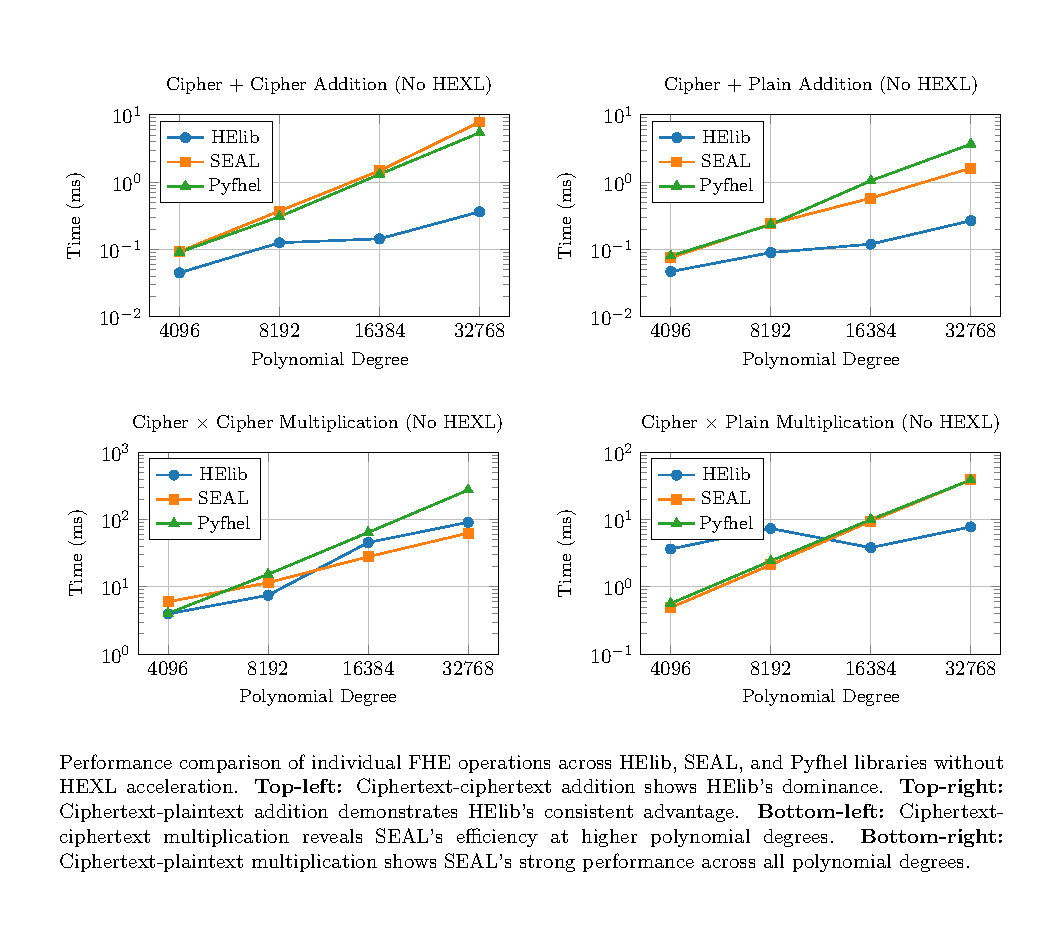
\includegraphics[width=\textwidth]{Images/atithematic_plot.pdf}
\caption{Experiment 1: Arithmetic Operation Latency Comparison Across SEAL,
HElib, and Pyfhel at Polynomial Degree 4096, with and without Intel HEXL
acceleration.}
\label{fig:exp1_arith}
\end{figure}

\begin{figure}[!ht]
\centering
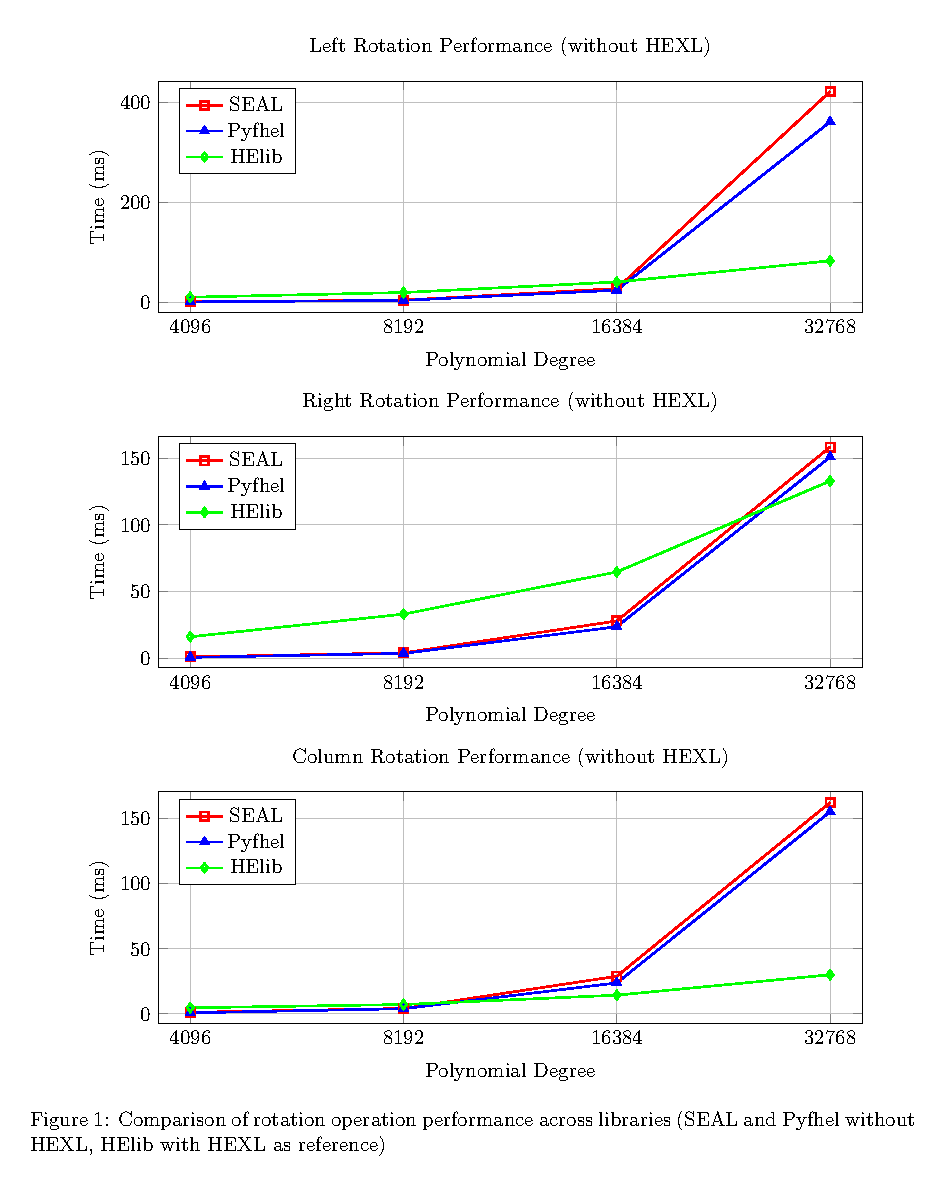
\includegraphics[width=\textwidth]{Images/rotation_comparison (2).pdf}
\caption{Experiment 2: Left Rotation Latency Scaling with Polynomial Degree
Across Libraries. SEAL exhibits super-linear scaling while HElib scales
approximately linearly.}
\label{fig:exp2_rotation}
\end{figure}

\begin{figure}[!ht]
\centering
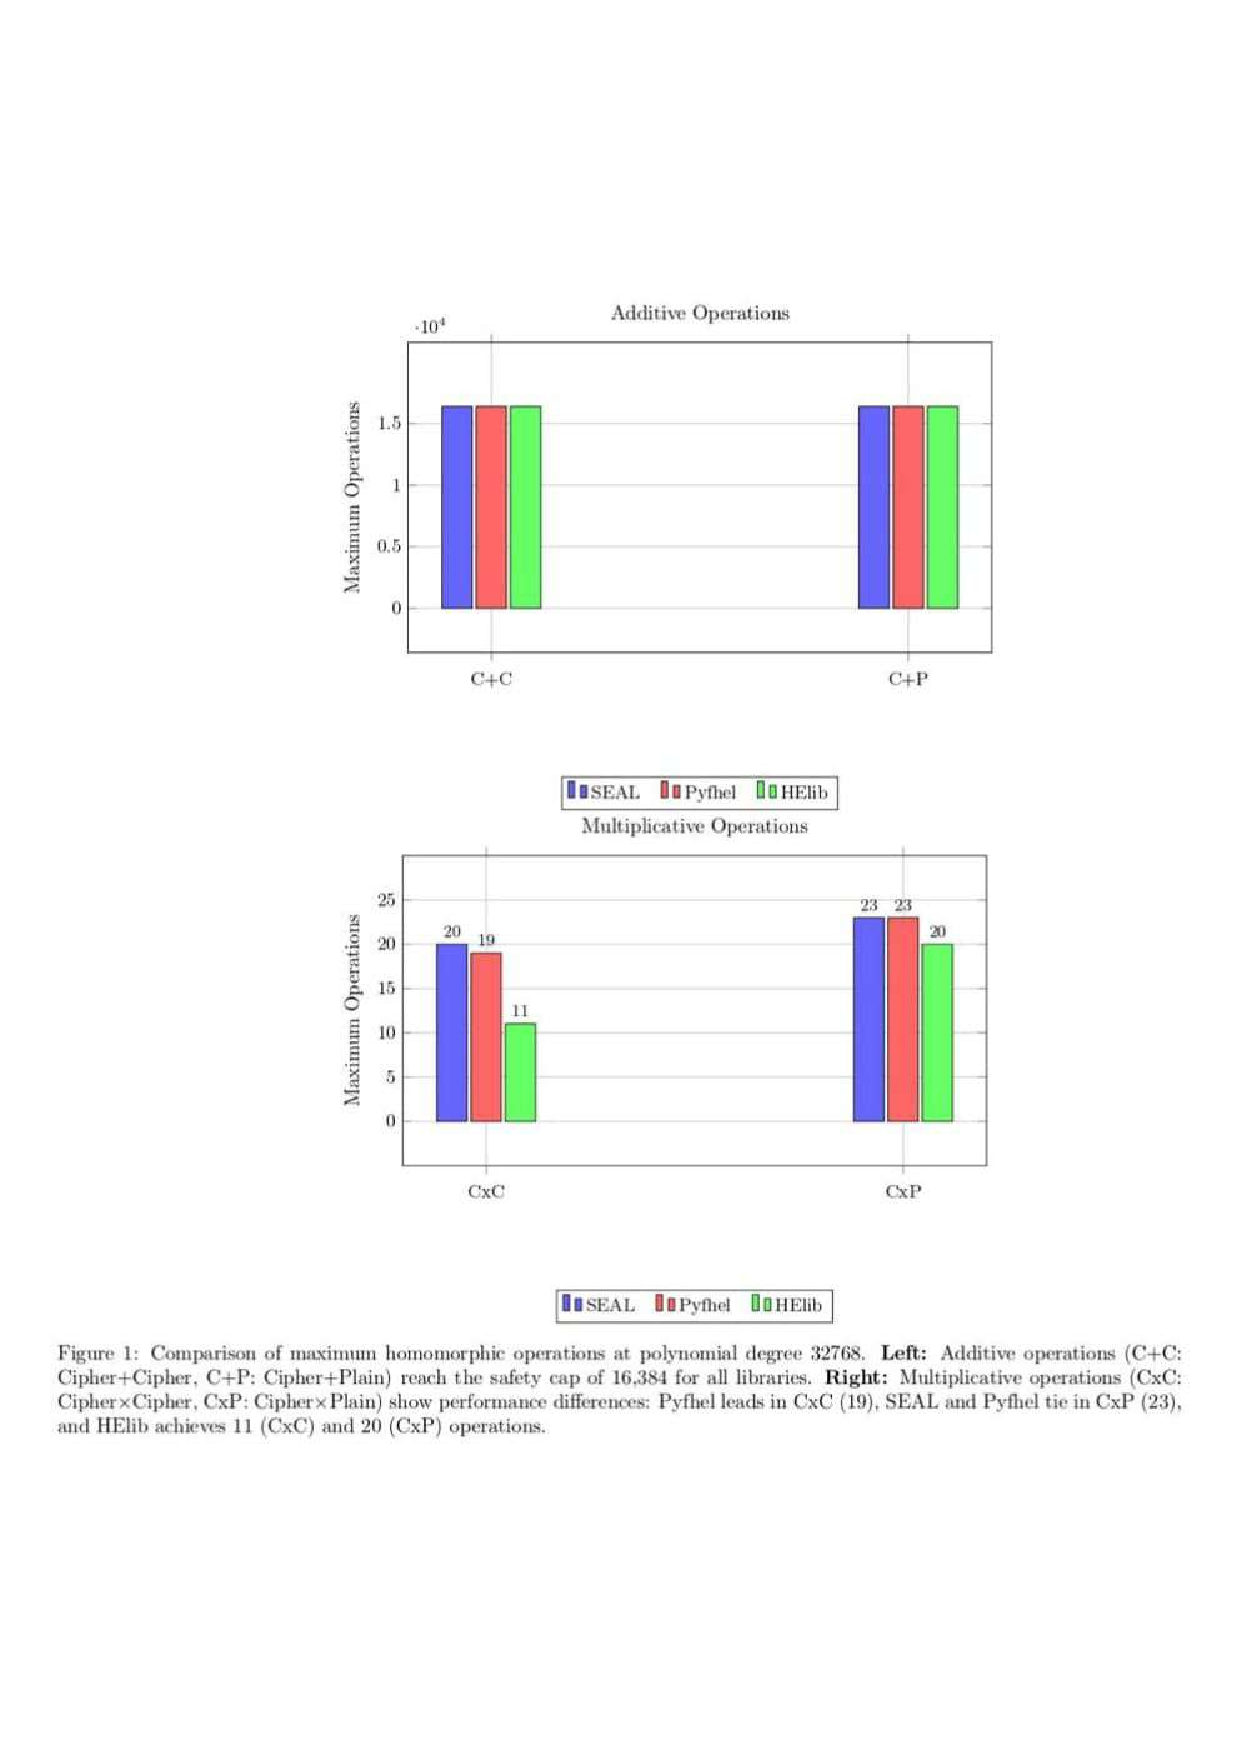
\includegraphics[width=\textwidth]{Images/depth_analysis.pdf}
\caption{Experiment 3: Maximum ct$\times$ct Multiplication Depth Before
Decryption Failure. SEAL achieves the deepest multiplication budget at all
polynomial degrees.}
\label{fig:exp3_depth}
\end{figure}

\begin{figure}[!ht]
\centering
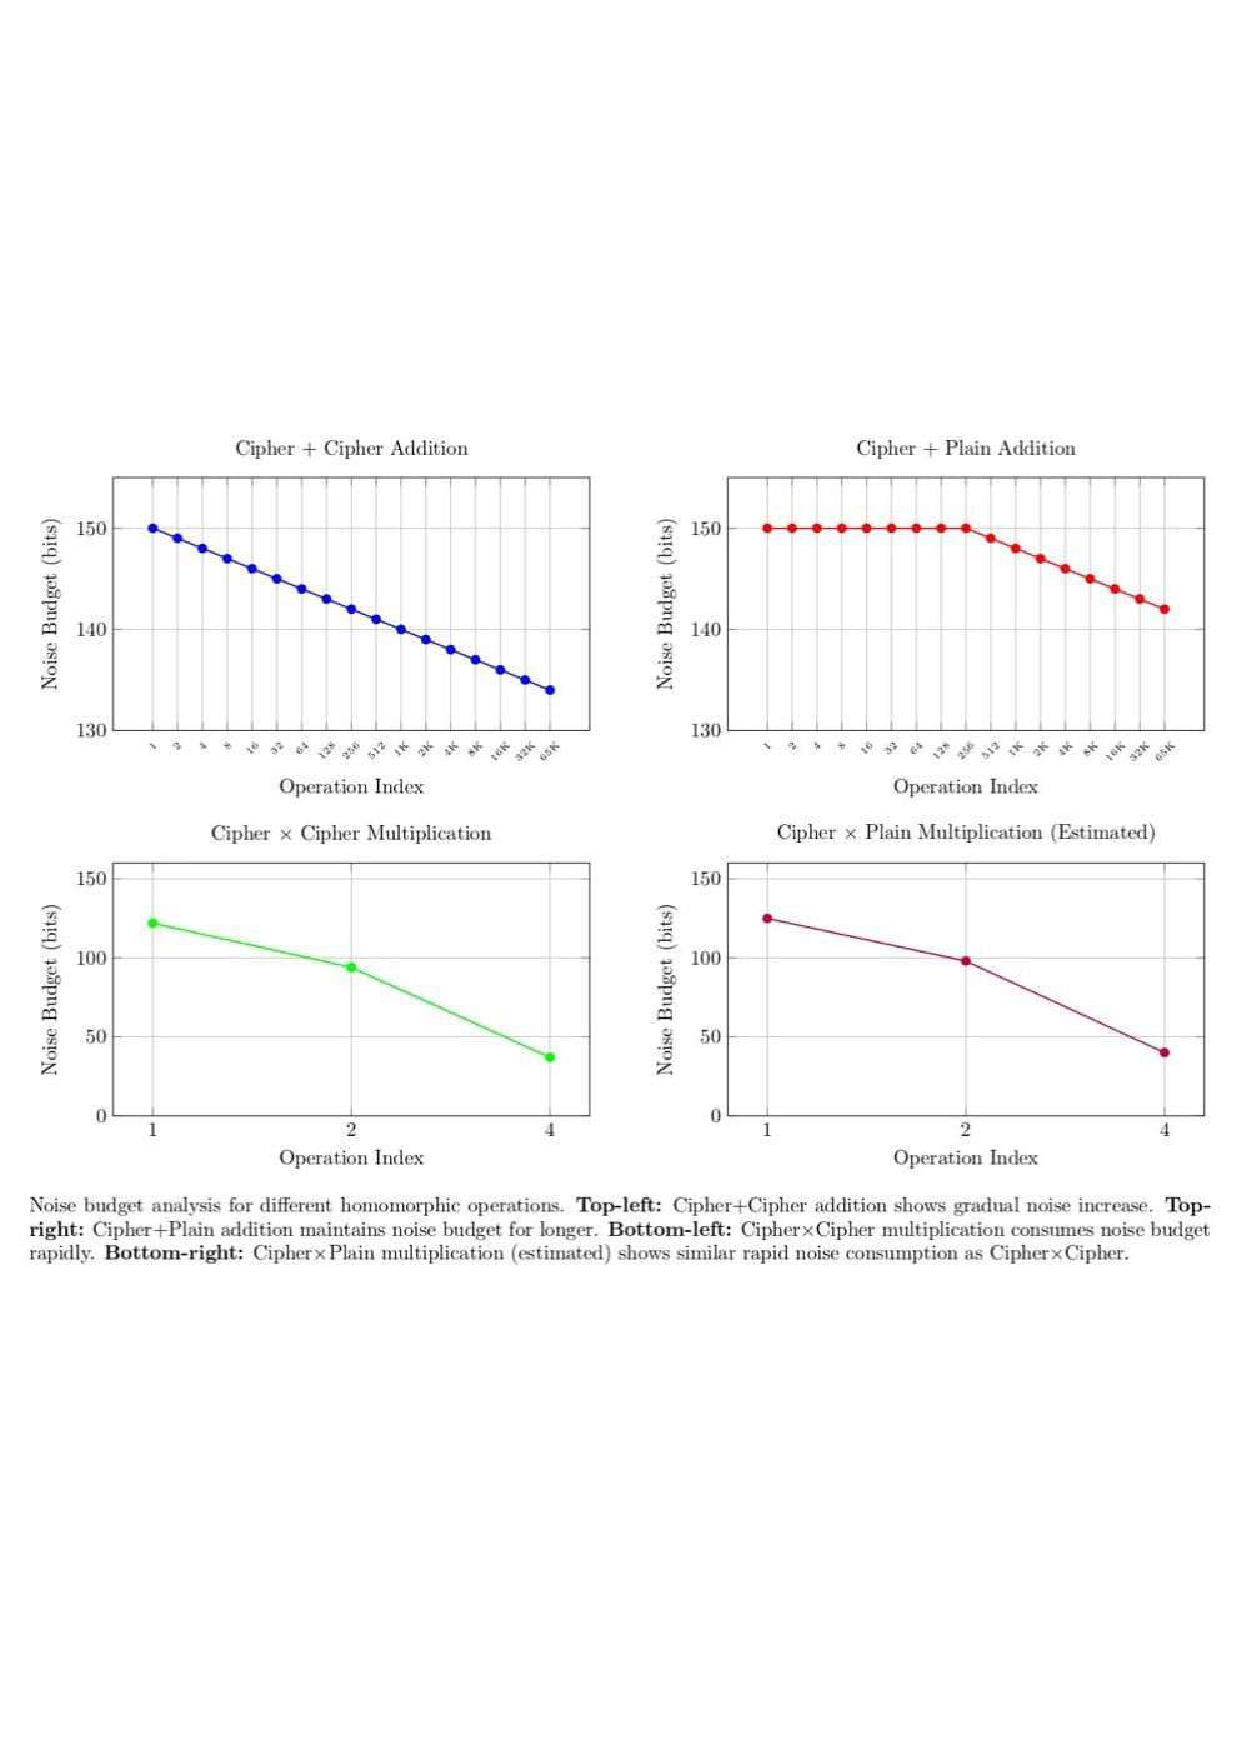
\includegraphics[width=\textwidth]{Images/noise_analysis.pdf}
\caption{Experiment 4: Noise Budget Evolution with Successive Multiplication
Operations. Each multiplication consumes approximately $1/L$ of the remaining
budget, directly motivating depth-efficient algorithm design.}
\label{fig:exp4_noise}
\end{figure}
\chapter{System Design: Preprocessing Pipeline and Encrypted Division Protocol}
\chaptermark{System Design}
\HRule\\[2cm]
\label{Chapter4}
\lhead{\emph{\textbf{Chapter 4:} System Design}}

\begin{spacing}{1.6}

\section{System Architecture}

\subsection{Privacy Model and Threat Model}

The system is designed under an \textit{honest-but-curious} adversary model:
the detection server follows the protocol specification correctly but may
attempt to infer information about individual data points from the ciphertexts
it receives, the intermediate computations it performs, and the values it
returns to the client.

The privacy guarantee enforced throughout all protocol phases is as follows:

\begin{itemize}
  \item The \textbf{data owner (client)} holds the raw plaintext data, the
  secret decryption key $\mathbf{sk}$, and all final anomaly classification
  decisions. The client is the only entity that can decrypt any ciphertext.

  \item The \textbf{detection server} holds the public encryption key
  $\mathbf{pk}$, the relinearization keys $\mathbf{rlk}$ (used to reduce
  degree-2 ciphertexts after multiplication back to degree-1), and the Galois
  rotation keys $\mathbf{galk}$ (used for slot vector rotations). The server
  holds encrypted ciphertexts and performs all HE computation but
  \textbf{never} holds $\mathbf{sk}$.

  \item No individual data point is ever revealed to the server at any protocol
  step. The server only computes on ciphertexts.

  \item During the inversion rounds, the client receives only aggregate model
  parameters: $N$ (the number of training rows) and $\sigma_j^2$ (per-feature
  variance). These are global statistics over the entire training model 
  functionally equivalent to the stored parameters of a deployed ML model 
  not individual data points. Their disclosure does not expose any individual
  training observation.
\end{itemize}

\subsection{Three-Process Architecture}

The complete system is implemented as three independent processes:

\textbf{Process 1 --- Detection Server (FastAPI):}
Receives encrypted ciphertexts from the client via HTTP REST endpoints. Performs
all HE computation: slot sums, mean computation, variance derivation, PCA
fitting (in plaintext on the component matrix $\mathbf{V}$), and anomaly score
computation. Maintains a \texttt{ServerState} object that persists encrypted
intermediate values (training ciphertexts, computed means, inverse variances,
test ciphertexts) across multiple HTTP requests. The server holds only
$\mathbf{pk}$, $\mathbf{rlk}$, and $\mathbf{galk}$ (never $\mathbf{sk}$).
Score computation runs asynchronously in a background thread to prevent HTTP
timeout for large test sets.

\textbf{Process 2 --- Data Owner Client (embedded in Dashboard):}
Encrypts data using $\mathbf{pk}$, participates in inversion rounds (decrypts
aggregate parameters using $\mathbf{sk}$, computes exact reciprocals in
plaintext, re-encrypts using $\mathbf{pk}$), receives encrypted score
ciphertexts from the server, decrypts them using $\mathbf{sk}$, applies the
anomaly threshold, and computes evaluation metrics. All decryption operations
occur exclusively on the client.

\textbf{Process 3 --- Monitoring Dashboard (Flask + SocketIO):}
A live webbased monitoring interface that embeds the client logic, eliminating
the need for a separate client terminal. Browser buttons communicate via
SocketIO events to the dashboard backend, which spawns background threads to
execute client protocol operations. The dashboard displays real time protocol
progress, per round latency, score distributions, and classification metrics.

\subsection{Complete Module Structure}

\end{spacing}
\begin{table}[!ht]
\centering
\caption{Complete System Modules and Their Responsibilities}
\label{tab:modules}
\begin{tabular}{p{5cm}p{8cm}}
\toprule
\textbf{Module} & \textbf{Responsibility} \\
\midrule
\texttt{key.py} & SEAL context initialization, key generation (pk, sk, rlk, galk), key persistence \\
\texttt{shared/config.py} & Centralized configuration: network ports, file paths, SEAL parameters, protocol constants \\
\texttt{shared/protocol.py} & Base64 serialization/deserialization of SEAL ciphertexts for HTTP JSON transport \\
\texttt{client/encrypt.py} & Column-major training ciphertext creation; row-major test ciphertext creation; scaler application \\
\texttt{client/decrypt.py} & Scalar single-value decryption; vector multi-value decryption \\
\texttt{client/invert.py} & Exact $1/x$ computation in plaintext and CKKS re-encryption \\
\texttt{client/decide.py} & Threshold classification; AUC, F1, Precision, Recall, confusion matrix computation \\
\texttt{client/http\_client.py} & HTTP client implementing all SAD and PCA protocol rounds over REST \\
\texttt{server/algo.py} & HE-SAD: slot sums, mean computation, sigma² computation, SAD score computation \\
\texttt{server/pca\_algo.py} & HE-PCA: slot sums, mean computation, PCA fitting, optimal $k^*$ selection, reconstruction error scoring \\
\texttt{server/http\_server.py} & FastAPI REST server, ServerState machine, async score computation, results management \\
\texttt{dashboard/dashboard\_app.py} & Flask + SocketIO dashboard; embedded client controller; browser button event handlers \\
\texttt{dashboard/templates/dashboard.html} & Live monitoring UI: buttons, progress bar, round status, latency charts, metrics display \\
\texttt{sad\_baseline.py} & Plaintext SAD reference implementation for performance comparison \\
\texttt{pca\_baseline.py} & Plaintext PCA reference implementation without StandardScaler \\
\bottomrule
\end{tabular}
\end{table}

\begin{spacing}{1.6}
    
\end{spacing}

\section{Dataset-Agnostic Preprocessing Pipeline}

\subsection{Design Philosophy}

The preprocessing pipeline converts raw multivariate data from any domain into
CKKS-compatible normalized form. Three constraints drive the design:

\textbf{CKKS compatibility:} All feature values must lie within $[-1, 1]$ after
normalization. CKKS encodes plaintext vectors as polynomial coefficients scaled
by $2^{40}$. Values outside $[-1, 1]$ cause coefficient overflow, and values
far from zero amplify noise relative to signal. The normalization step is
therefore not merely a conventional ML preprocessing step but a CKKS correctness
requirement.

\textbf{Information separation:} All normalization parameters must be computed
exclusively from normal training data. If min/max values were computed from
data including attack rows, extreme attack-induced values would expand the
normalization range, compressing all normal values into a narrow band near zero
and reducing detection sensitivity. The pipeline enforces strict separation
between training statistics and test data.

\textbf{Feature type awareness:} Datasets contain heterogeneous feature types
--- continuous analog sensor readings and discrete binary actuator states. These
require different normalization strategies to maintain appropriate value ranges
and to ensure each feature type contributes meaningfully to anomaly scoring.

\subsection{Stage 1: Structural Cleaning}

The first stage removes all metadata columns that carry no sensor signal and
would corrupt the numeric feature matrix:

\begin{itemize}
  \item \textbf{Timestamp columns} (\texttt{Timestamp} in SWaT,
  \texttt{DATETIME} in BATADAL): Date-time strings cannot be meaningfully
  encoded as real valued features and carry no anomaly discriminating information.
  \item \textbf{Label columns} (\texttt{Normal/Attack} in SWaT,
  \texttt{ATT\_FLAG} in BATADAL): Ground truth labels are retained separately
  for evaluation but excluded from all feature processing, ensuring the system
  remains unsupervised.
\end{itemize}

After cleaning, SWaT retains 51 feature columns and BATADAL retains 43,
consisting purely of numeric sensor and actuator readings.

\subsection{Stage 2: Missing Value Resolution}

The second stage fills gaps in the numeric feature matrix using a three-pass
imputation strategy:

\textbf{Pass 1 --- Forward fill:} The last valid observation for each feature
is propagated forward to fill subsequent gaps. This is the physically appropriate
assumption for time series sensor data: a missing reading most likely reflects
a sensor reporting its last known state, since physical quantities such as water
level, pressure, and flow rate change continuously and cannot jump discontinuously.

\textbf{Pass 2 --- Backward fill:} Any gaps remaining at the beginning of the
recording period (where no prior valid observation exists to propagate forward)
are resolved by propagating the next valid observation backward.

\textbf{Pass 3 --- Column mean fill:} As a last resort, any gaps persisting
after both passes are filled with the column mean. In practice, both SWaT and
BATADAL required only the first two passes, with post resolution verification
confirming zero remaining missing values.

A programmatic check (\texttt{np.isnan(X).sum() == 0}) confirms successful
imputation before proceeding.

\subsection{Stage 3: Feature Type Classification}

Each feature is automatically classified as continuous or binary based on its
observed value distribution in the training data:

\textbf{Continuous features} are real-valued analog sensor readings that vary
smoothly over time. Examples include:
\begin{itemize}
  \item Flow rates (FIT/F\_PU sensors): measure volumetric flow in litres per
  second, ranging from near-zero to several hundred.
  \item Water levels (LIT/L\_T sensors): measure absolute level in millimetres
  or centimetres.
  \item Pressures (PIT/P\_J sensors): measure differential or absolute pressure
  in appropriate units.
\end{itemize}

\textbf{Binary features} are discrete indicators recording the on/off or
open/closed state of digital actuators. Examples include:
\begin{itemize}
  \item Pump on/off signals (P/S\_PU sensors): 0 = off, 1 = on.
  \item Motorized valve positions (MV/S\_V sensors): 0 = closed, 1 = open.
\end{itemize}

SWaT contains 26 continuous and 25 binary features; BATADAL contains 28
continuous and 15 binary features.

\subsection{Stage 4: CKKS-Compatible Normalization}

\subsubsection{Continuous Feature Normalization}

Each continuous feature $x_i$ is linearly scaled to $[-1, 1]$ using the
minimum and maximum values observed across all \textit{normal} training rows:
\begin{equation}
  x'_i = \frac{2(x_i - x_{\min})}{x_{\max} - x_{\min}} - 1
  \label{eq:normalization}
\end{equation}
where $x_{\min}$ and $x_{\max}$ are computed from normal training rows only.
The scaled value equals $-1$ at the minimum observed normal value, $+1$ at the
maximum, and $0$ at the midpoint of the normal operating range.

In cases where $x_{\max} = x_{\min}$ (a constant feature), the denominator is
replaced by $1$ to avoid division by zero, and the feature is assigned value $0$.
The per-feature $(x_{\min}, x_{\max})$ pairs are serialized to
\texttt{scaler.npy} for consistent application to test data.

\subsubsection{Binary Feature Normalization}

Binary actuator state features are remapped from their original $\{0, 1\}$
representation to $\{-1, +1\}$:
\begin{equation}
  x'_i = 2x_i - 1
  \label{eq:binary_norm}
\end{equation}

Two considerations motivate this remapping:

\textit{Uniform feature space:} Remapping brings binary features into the same
$[-1, +1]$ value space as normalized continuous features. When all $d$ features
are packed into a single CKKS ciphertext slot vector, each feature occupies one
slot. If binary features retained their $\{0, 1\}$ range while continuous
features span $[-1, 1]$, the binary features would have systematically half the
magnitude, distorting the anomaly score contributions.

\textit{Symmetric anomaly contribution:} In the SAD score formula, the squared
deviation of a binary feature from its mean $\mu_j \in (-1, 1)$ is computed.
With $\{-1, +1\}$ values, both the off-state ($-1$) and the on-state ($+1$)
contribute nonzero squared deviations from any mean, ensuring that actuator
state anomalies (an unexpected pump activation or valve closure) register in
the anomaly score.

\subsection{Stage 5: Output Verification}

Five automated checks guard against silent preprocessing failures:
\begin{enumerate}
  \item Zero missing values: \texttt{np.isnan(X).sum() == 0}
  \item Continuous range: all values within $[-1.01, 1.01]$ (1\% tolerance for
  floating-point rounding at boundary values)
  \item Binary value set: each binary column contains only $\{-1, +1\}$
  \item Row count preservation: output row count equals input row count
  \item Column count: exactly 51 (SWaT) or 43 (BATADAL) columns
\end{enumerate}

Both datasets passed all five checks, producing verified output files used as
direct input to the CKKS encryption pipeline.

\begin{table}[H]
\centering
\caption{Preprocessing Pipeline Summary}
\label{tab:preproc}
\begin{tabular}{p{0.5cm}p{3.5cm}p{4.5cm}p{4.5cm}}
\toprule
\textbf{\#} & \textbf{Stage} & \textbf{SWaT} & \textbf{BATADAL} \\
\midrule
1 & Structural Cleaning & Remove Timestamp, Normal/Attack & Remove DATETIME, ATT\_FLAG \\
2 & Missing Values & Fwd $\to$ Bwd $\to$ Mean fill & Fwd $\to$ Bwd $\to$ Mean fill \\
3 & Feature Classification & 26 continuous, 25 binary & 28 continuous, 15 binary \\
4a & Continuous Norm. & Min-max to $[-1,1]$ from normal rows & Min-max to $[-1,1]$ from normal rows \\
4b & Binary Norm. & $\{0,1\} \to \{-1,+1\}$ & $\{0,1\} \to \{-1,+1\}$ \\
5 & Verification & 5 checks, all passed & 5 checks, all passed \\
\bottomrule
\end{tabular}
\end{table}

\section{CKKS Encoding Strategies}

Two distinct encoding strategies are used for training data and test data,
each optimised for the operations performed on them.

\subsection{Column-Major Training Encoding}

Training data is encoded one ciphertext per feature, packing all $N$ training
row values for that feature into the SIMD slots:
\begin{equation}
  \mathrm{ct}_j^{\text{train}} = \mathrm{Enc}_\mathbf{pk}
  ([x_{0j}, x_{1j}, x_{2j}, \ldots, x_{N-1,j}])
  \quad \text{for } j = 1, \ldots, d
  \label{eq:colmajor}
\end{equation}

This encoding enables the computation of the feature column sum using a
binary rotation tree: summing $N$ slot values requires only $\lceil\log_2 N
\rceil$ rotate-and-add steps. For $N = 5000$ training rows, this requires 13
rotations rather than 4999 sequential additions, reducing noise accumulation
and computation time by orders of magnitude.

The column sum $\sum_{i=0}^{N-1} x_{ij}$ (present in all slots after the
rotation tree) is used to compute the feature mean $\mu_j = \frac{1}{N}
\sum_i x_{ij}$ after division by $N$ via the multi-round protocol.

\subsection{Row-Major Test Encoding}

Test data is encoded one ciphertext per test observation, packing all $d$
feature values into slots $0$ through $d-1$, with slots $d$ through $n/2-1$
zero-padded:
\begin{equation}
  \mathrm{ct}_i^{\text{test}} = \mathrm{Enc}_\mathbf{pk}
  ([x_{i0}, x_{i1}, \ldots, x_{i,d-1}, 0, 0, \ldots, 0])
  \quad \text{for } i = 1, \ldots, N_\text{test}
  \label{eq:rowmajor}
\end{equation}

This encoding enables anomaly score computation for observation $i$ in a single
HE evaluation: subtract the mean vector (sub\_plain), square element-wise
(square), multiply by the inverse variance vector (mult\_plain), and sum all
$d$ slot values using $\lceil\log_2 d\rceil$ rotate-and-add steps. For
$d = 51$ features, only 6 rotations are required.

The zero padding in slots $d$ through $n/2-1$ contributes zero to the slot
sum, so the anomaly score for the row is correctly accumulated in slot 0 of
the result ciphertext.

\section{The Encrypted Division Problem}

\subsection{Problem Statement}

The CKKS scheme natively supports ciphertext-ciphertext addition and
multiplication, and ciphertext-plaintext addition and multiplication. It does
not natively support division. This limitation is fundamental: division is
a non-polynomial function and cannot be computed exactly using a finite number
of multiplications.

Both SAD and PCA require division at critical protocol steps:
\begin{itemize}
  \item \textbf{Computing the feature mean:} $\mu_j = \frac{1}{N} \sum_i
  x_{ij}$ requires dividing the column sum by $N$.
  \item \textbf{SAD variance normalization:} $s(\mathbf{x}) = \sum_j
  \frac{(x_j-\mu_j)^2}{\sigma_j^2}$ requires dividing by $\sigma_j^2$ for each
  of $d = 51$ features.
\end{itemize}

Without division, these fundamental statistics cannot be computed, and the
anomaly detection algorithms cannot be faithfully implemented under encryption.

Three approaches to encrypted division were evaluated: Newton-Raphson iterative
inversion, Chebyshev polynomial approximation, and a novel multi-round
interactive protocol.

\subsection{Approach 1: Newton-Raphson Iterative Inversion}

The Newton-Raphson method for computing $1/a$ is the iterative formula:
\begin{equation}
  y_{n+1} = y_n(2 - a \cdot y_n)
  \label{eq:nr}
\end{equation}

Under the convergence condition $|1 - a \cdot y_0| < 1$, this sequence
converges quadratically to $1/a$ starting from the initial guess $y_0$. Each
iteration requires two multiplications (computing $a \cdot y_n$ and
$y_n \cdot (2 - a \cdot y_n)$), consuming 2 HE levels per iteration.

Applied to computing $1/\sigma_j^2$ for all 51 features simultaneously under
CKKS, the 51 variance values are packed into the 51 slots of a single
ciphertext, and the iteration runs element wise across all slots simultaneously.

\textbf{Experimental results on SWaT variance values:}

The SWaT training data produces feature variances $\sigma_j^2 \in [0.012,
0.45]$, spanning a $37\times$ range from smallest to largest. A single initial
guess $y_0$ must work for all 51 slots simultaneously:

\begin{table}[H]
\centering
\caption{Newton-Raphson Convergence on SWaT $\sigma^2 \in [0.012, 0.45]$}
\label{tab:nr}
\begin{tabular}{cccc}
\toprule
\textbf{Iter.} & \textbf{$y_0 = 4.33$ (1/median)} & \textbf{Mean Error} & \textbf{Status} \\
\midrule
0 & Initial guess & 59.8\% & Single guess for all 51 slots \\
1 & $y_1 = y_0(2-ay_0)$ & 187.2\% & Diverging \\
2 & $y_2 = y_1(2-ay_1)$ & 941.1\% & Fully diverged \\
3 & $y_3 = y_2(2-ay_2)$ & 5594.3\% & Unusable \\
\bottomrule
\end{tabular}
\end{table}

\textbf{Root cause of divergence:} The convergence condition requires
$|1 - a \cdot y_0| < 1$, equivalently $y_0 \in (0, 2/a)$. For a single
initial guess $y_0 = 4.33$ (the reciprocal of the median variance):
\begin{itemize}
  \item For the maximum variance feature ($\sigma^2 = 0.45$): $a \cdot y_0
  = 0.45 \times 4.33 = 1.95$, giving $|1 - 1.95| = 0.95 < 1$. Convergent
  but slow.
  \item For the minimum variance feature ($\sigma^2 = 0.012$): $a \cdot y_0
  = 0.012 \times 4.33 = 0.052$, giving $|1 - 0.052| = 0.948 < 1$.
  Technically convergent, but the $37\times$ range means many features
  are near the boundary of convergence while others diverge under the
  combined SIMD iteration.
\end{itemize}

Per slot initial guesses assigning $y_0^{(j)} = 1/\sigma_j^2$ to each slot
independently  would solve this problem, but CKKS does not support
slot-selective initial assignments in a way that avoids the underlying
arithmetic instability when all slots evolve under the same iteration formula.

\textbf{Conclusion:} Newton-Raphson inversion is not viable for encrypted
division across heterogeneous variance values.

\subsection{Approach 2: Chebyshev Polynomial Approximation}

A degree-$n$ Chebyshev polynomial is fitted offline to approximate $1/x$ on
the interval $[x_{\min}, x_{\max}]$ using Chebyshev nodes to minimize the
Runge phenomenon. The polynomial is then evaluated inside the HE computation
by substituting the ciphertext for $x$.

\begin{table}[H]
\centering
\caption{Chebyshev Approximation of $1/x$ on $[0.012, 0.45]$}
\label{tab:cheb}
\begin{tabular}{cccl}
\toprule
\textbf{Degree} & \textbf{Plaintext Error} & \textbf{HE Levels} & \textbf{HE Status} \\
\midrule
3 & 33.3\% & 2--3 & Executed; error unacceptable \\
5 & 19.1\% & 3--4 & Scale overflow \\
7 & 8.5\%  & 3--4 & Scale overflow \\
9 & 5.4\%  & 4--5 & Scale overflow \\
\bottomrule
\end{tabular}
\end{table}

\textbf{Analysis of results:}

At degree 3, the polynomial executes but produces a mean approximation error
of 33.3\% across the variance range. Substituting $1/\sigma_j^2$ with a value
33\% in error means the anomaly score for each feature deviates by 33\% from
the correct normalised squared deviation. This completely destroys the score
separation between normal and anomalous observations, making degree-3 Chebyshev
unusable.

At degrees 5, 7, and 9, scale overflow occurs. The root cause: each Chebyshev
basis polynomial $T_k(x)$ must be evaluated by multiplying the plaintext
polynomial coefficients with the current ciphertext level. The plaintext was
encoded at the global scale $2^{40}$, but after several rescaling operations
the ciphertext operates at a smaller effective scale determined by the remaining
prime size. Multiplying a plaintext encoded at $2^{40}$ by a ciphertext at a
reduced scale produces a product with scale far exceeding the current prime
capacity, causing overflow.

Encoding the plaintext at the ciphertext's current scale (\texttt{ct.scale()}
rather than the global \texttt{SCALE}) resolves the overflow but reduces the
polynomial evaluation precision, and degree 3 remains the only depth-feasible
option, with unacceptable 33.3\% error.

\textbf{Conclusion:} Chebyshev polynomial approximation is not viable for
encrypted division in this application.

\subsection{Approach 3: Multi-Round Interactive Protocol (Adopted)}

The multi-round interactive protocol resolves the encrypted division problem
by routing the computation of the reciprocal through the key holding data owner,
who can perform exact division in plaintext.

The protocol for computing $\mathrm{ct}_{1/a}$ from $\mathrm{ct}_a$ is:

\begin{enumerate}
  \item The server computes and sends $\mathrm{ct}_a$ to the client.
  \item The client decrypts using $\mathbf{sk}$: $a = \mathrm{Dec}_\mathbf{sk}
  (\mathrm{ct}_a)$.
  \item The client computes the exact reciprocal in plaintext:
  $r = 1.0 / a$ (IEEE 754 double precision).
  \item The client encodes $r$ and re-encrypts using $\mathbf{pk}$:
  $\mathrm{ct}_r = \mathrm{Enc}_\mathbf{pk}(r)$.
  \item The client sends $\mathrm{ct}_r$ to the server, which continues the
  protocol using $\mathrm{ct}_r$ in subsequent multiplications.
\end{enumerate}

\begin{table}[H]
\centering
\caption{Comparison of Division Approaches}
\label{tab:div}
\begin{tabular}{p{3cm}cccp{3.5cm}}
\toprule
\textbf{Method} & \textbf{Error} & \textbf{HE Levels} & \textbf{Works} & \textbf{Limitation} \\
\midrule
Newton-Raphson & Diverges & 6 per attempt & No & Wide variance range causes divergence \\
Chebyshev d=3 & 33.3\% & 2--3 & No & Error too large for anomaly detection \\
Chebyshev d$\geq$5 & $<$20\% & 3--5 & No & Scale overflow in HE \\
\textbf{Multi-Round} & \textbf{0\%} & \textbf{0} & \textbf{Yes} & None \\
\bottomrule
\end{tabular}
\end{table}

\textbf{Privacy analysis:} The protocol reveals to the client only the value
$a$ that was decrypted. In the SAD protocol, this is either:
\begin{itemize}
  \item $N = 5000$ (the number of training rows): reveals only the dataset
  size, which is a public protocol parameter, not a data point.
  \item $\sigma_j^2$ for $j = 1, \ldots, 51$: the feature variances over the
  training set. These are global statistics computed over all 5000 training
  rows, equivalent in sensitivity to the stored parameters of a trained
  scikit-learn model. They do not reveal any individual training observation
  or its label.
\end{itemize}

The protocol introduces two additional communication rounds but adds zero HE
multiplication levels, preserving the full 5-level budget for the actual anomaly
scoring computation.

\textbf{Conclusion:} The multi-round interactive protocol achieves exact
encrypted division with zero approximation error and zero HE depth cost, making
it the only viable approach for this application.

\end{spacing}

\chapter{Privacy-Preserving Anomaly Detection: Implementation and Results}
\chaptermark{Implementation and Results}
\HRule\\[2cm]
\label{Chapter5}
\lhead{\emph{\textbf{Chapter 5:} Implementation and Results}}

\begin{spacing}{1.6}

% ─────────────────────────────────────────────────────────────
\section{HE-SAD: Homomorphic Statistical Anomaly Detection}
% ─────────────────────────────────────────────────────────────

\subsection{Algorithm Design Under CKKS Constraints}

The SAD anomaly score (Equation~\ref{eq:sad}) decomposes into four operations
that must be executed under CKKS encryption for each test ciphertext:

\begin{enumerate}
  \item \textbf{Centering:} Subtract the plaintext mean vector from the
  encrypted test row. Since $\boldsymbol{\mu}$ is a plaintext vector (computed
  from the multi-round protocol result and known to the server), this is a
  \texttt{sub\_plain} operation.
  \begin{equation}
    \mathrm{ct}_{xc} \leftarrow \mathrm{ct}_i - \mathrm{pt}_\mu
    \quad \text{(0 levels consumed)}
  \end{equation}

  \item \textbf{Squaring:} Square the centred ciphertext element-wise to
  compute $(x_j - \mu_j)^2$ for all $j$ simultaneously.
  \begin{equation}
    \mathrm{ct}_{sq} \leftarrow \mathrm{ct}_{xc}^2
    \xrightarrow{\text{relinearize}} \xrightarrow{\text{rescale}}
    \quad \text{(1 level consumed)}
  \end{equation}
  After squaring, the ciphertext scale doubles to $2^{80}$. Relinearization
  reduces the degree-2 result back to degree-1 format. Rescaling divides by
  the last prime in the modulus chain, returning to scale $2^{40}$ and
  consuming one level.

  \item \textbf{Variance normalisation:} Multiply element-wise by the
  plaintext vector of inverse variances $1/\sigma_j^2$.
  \begin{equation}
    \mathrm{ct}_{sc} \leftarrow \mathrm{ct}_{sq} \cdot
    \mathrm{pt}_{1/\sigma^2}
    \xrightarrow{\text{rescale}}
    \quad \text{(1 level consumed)}
  \end{equation}
  The plaintext $\mathrm{pt}_{1/\sigma^2}$ must be encoded at the
  ciphertext's current scale to avoid scale mismatch errors.

  \item \textbf{Slot summation:} Sum all $d$ slot values to obtain the
  scalar anomaly score in slot~0.
  \begin{equation}
    \mathrm{ct}_{score} \leftarrow
    \sum_{k=0}^{\lceil\log_2 d\rceil - 1}
    \mathrm{Rot}(\mathrm{ct}_{sc}, 2^k) + \mathrm{ct}_{sc}
    \quad \text{(0 levels, 6 rotations)}
  \end{equation}
  The binary rotation tree sums $d$ slot values using
  $\lceil\log_2 d\rceil$ rotate-and-add steps.
  Zero-padded slots contribute nothing to the sum.
\end{enumerate}

Table~\ref{tab:sad_depth} summarises the HE depth consumed per test row.

\end{spacing}

\begin{table}[!ht]
\centering
\caption{HE-SAD Per-Row Computation Depth Budget (5 levels available)}
\label{tab:sad_depth}
\begin{tabular}{p{4cm}p{5cm}cc}
\toprule
\textbf{Operation} & \textbf{SEAL Method} & \textbf{Levels} & \textbf{Rotations} \\
\midrule
$\mathbf{x}_i - \boldsymbol{\mu}$ &
  \texttt{sub\_plain(ct\_i, pt\_mu)} & 0 & 0 \\
$(x_j - \mu_j)^2$ &
  \texttt{square}, \texttt{relinearize}, \texttt{rescale} & 1 & 0 \\
$\times\,1/\sigma_j^2$ &
  \texttt{multiply\_plain}, \texttt{rescale} & 1 & 0 \\
$\sum_{j=1}^{d}$ &
  \texttt{rotate\_and\_add} $\times\,\lceil\log_2 d\rceil$ & 0 & 6 \\
\midrule
\textbf{Total per row} & & \textbf{2 of 5} & \textbf{6} \\
\bottomrule
\end{tabular}
\end{table}

\begin{spacing}{1.6}

\subsection{The Nine-Round HE-SAD Protocol}

The complete protocol is shown in Table~\ref{tab:sad_proto}, and the full
client--server state-transition diagram is presented in
Figure~\ref{fig:sad_protocol}.

\end{spacing}

\begin{table}[!ht]
\centering
\caption{Complete HE-SAD Protocol}
\label{tab:sad_proto}
\begin{tabular}{p{0.6cm}p{2.8cm}p{7.2cm}p{2.5cm}}
\toprule
\textbf{Rnd} & \textbf{Operation} & \textbf{Details} & \textbf{Direction} \\
\midrule
1 & Upload training data &
  Column-major ciphertexts ($\approx$51\,MB); one per feature with all
  $N$ training row values in SIMD slots &
  Client $\to$ Server \\[4pt]
2 & Compute column sums &
  Server applies binary rotation tree (13 rotations per feature);
  returns $\mathrm{ct}_N$ encoding $N$ in all slots &
  Server $\to$ Client \\[4pt]
3 & Invert $N$ &
  Client decrypts $\mathrm{ct}_N$, computes exact $1/N$ in plaintext,
  re-encrypts as $\mathrm{ct}_{1/N}$ &
  Client $\to$ Server \\[4pt]
4 & Compute $\mu$ and $\sigma^2$ &
  Server computes $\mathrm{ct}_{\mu_j} = \mathrm{ct}_{\mathrm{sum},j}
  \cdot \mathrm{ct}_{1/N}$; derives $\mathrm{ct}_{\sigma^2_j}$ from
  training ciphertexts; sends packed $\mathrm{ct}_{\sigma^2}$ to client &
  Server $\to$ Client \\[4pt]
5 & Invert $\sigma^2$ &
  Client decrypts all $d$ variance values; computes exact
  $1/\sigma_j^2$; re-encrypts as packed $\mathrm{ct}_{1/\sigma^2}$ &
  Client $\to$ Server \\[4pt]
6 & Upload test data &
  Row-major ciphertexts uploaded in batches of 100 per HTTP POST
  ($\approx$100\,MB per batch) &
  Client $\to$ Server \\[4pt]
7 & Compute SAD scores &
  Server scores all test ciphertexts asynchronously in a background
  thread; 2 HE levels consumed per row &
  Server (async) \\[4pt]
8 & Fetch scores &
  Client polls \texttt{/api/scores/status} every 5\,s; fetches
  encrypted scores in batches of 100 &
  Server $\to$ Client \\[4pt]
9 & Decrypt and classify &
  Client decrypts all score ciphertexts using $\mathbf{sk}$; applies
  threshold $\tau = \bar{s}_\mathrm{train} + 3\sigma_{s,\mathrm{train}}$;
  computes AUC, F1, Precision, Recall &
  Client (local) \\
\bottomrule
\end{tabular}
\end{table}

\begin{figure}[!ht]
\centering
\includegraphics[width=\textwidth]{Images/he_sad_protocol.png}
\caption{HE-SAD nine-round protocol: full client--server state-transition
diagram showing internal state flow within each party and cross-network
message exchanges. The server holds only ciphertexts and public keys;
the secret key $\mathbf{sk}$ never leaves the client.}
\label{fig:sad_protocol}
\end{figure}

\begin{spacing}{1.6}

\subsection{Threshold Computation}

The detection threshold $\tau$ is computed from the normal training data
using the same HE-SAD scoring function:
\begin{equation}
  \tau = \bar{s}_\mathrm{train} + 3\,\sigma_{s,\mathrm{train}}
\end{equation}
Training rows are encrypted and scored through the live HE-SAD computation,
ensuring the threshold is calibrated to the actual HE score distribution
(which may differ slightly from plaintext SAD scores due to bounded CKKS
approximation noise $\approx 10^{-9}$) rather than to plaintext scores.

% ─────────────────────────────────────────────────────────────
\section{HE-PCA: Homomorphic Principal Component Analysis}
% ─────────────────────────────────────────────────────────────

\subsection{Algorithm Design Under CKKS Constraints}

The PCA reconstruction error (Equation~\ref{eq:pca}) requires five
operations per encrypted test row:

\begin{enumerate}
  \item \textbf{Centering:}
  \begin{equation}
    \mathrm{ct}_{xc} \leftarrow \mathrm{ct}_i - \mathrm{pt}_\mu
    \quad\text{(0 levels)}
  \end{equation}

  \item \textbf{Projection onto each component $k$:}
  \begin{equation}
    p_k = \langle \mathrm{ct}_{xc},\,\mathbf{v}_k \rangle
        = \mathrm{slot\_sum}\!\left(
            \mathrm{ct}_{xc} \cdot \mathrm{pt}_{\mathbf{v}_k}
          \right)
    \quad\text{(1 level)}
  \end{equation}

  \item \textbf{Reconstruction of component $k$:}
  \begin{equation}
    \mathrm{ct}_{r_k} = p_k \cdot \mathrm{pt}_{\mathbf{v}_k}
    \quad\text{(1 level)}
  \end{equation}
  The scalar $p_k$ (in slot~0 after the slot sum) is broadcast to all
  slots via a \texttt{multiply\_plain} with $\mathbf{v}_k$.

  \item \textbf{Residual:}
  \begin{equation}
    \mathrm{ct}_{res} = \mathrm{ct}_{xc}
      - \sum_{k=1}^{k^*} \mathrm{ct}_{r_k}
    \quad\text{(0 levels)}
  \end{equation}

  \item \textbf{Squared residual norm:}
  \begin{equation}
    \mathrm{ct}_{score} =
      \mathrm{slot\_sum}\!\left(\mathrm{ct}_{res}^2\right)
    \quad\text{(1 level + 6 rotations)}
  \end{equation}
\end{enumerate}

Table~\ref{tab:pca_depth} summarises the HE depth consumed per test row.

\end{spacing}

\begin{table}[!ht]
\centering
\caption{HE-PCA Per-Row Computation Depth Budget (5 levels available)}
\label{tab:pca_depth}
\begin{tabular}{p{4cm}p{5cm}cc}
\toprule
\textbf{Operation} & \textbf{SEAL Method} & \textbf{Levels} & \textbf{Rotations} \\
\midrule
$\mathbf{x}_i - \boldsymbol{\mu}$ &
  \texttt{sub\_plain} & 0 & 0 \\
$\langle\mathrm{ct}_{xc},\mathbf{v}_k\rangle$ &
  \texttt{multiply\_plain} + \texttt{rescale} + \texttt{slot\_sum} & 1 & 6 \\
$p_k \cdot \mathbf{v}_k$ &
  \texttt{multiply\_plain} + \texttt{rescale} & 1 & 0 \\
Residual &
  \texttt{sub} $\times\,k^*$ & 0 & 0 \\
$\|\mathrm{ct}_{res}\|^2$ &
  \texttt{square} + \texttt{rescale} + \texttt{slot\_sum} & 1 & 6 \\
\midrule
\textbf{Total per row} & & \textbf{3 of 5} & \textbf{12} \\
\bottomrule
\end{tabular}
\end{table}

\begin{spacing}{1.6}

\subsection{Optimal Component Selection}

The number of principal components $k^*$ is selected automatically using
the 90\% explained variance threshold:
\begin{equation}
  k^* = \min\!\left\{k :\;
    \frac{\sum_{i=1}^{k}\lambda_i}{\sum_{i=1}^{d}\lambda_i}
    \geq 0.90\right\}
\end{equation}
The server fits a full PCA on the plaintext training CSV (a public model
parameter, not individual data) and selects $k^*$ automatically.
Only the integer $k^*$ and the achieved variance ratio are reported to the
client; no raw feature values are revealed.

\subsection{The Eight-Round HE-PCA Protocol}

The complete protocol is shown in Table~\ref{tab:pca_proto}, and the full
client--server state-transition diagram is presented in
Figure~\ref{fig:pca_protocol}.

\end{spacing}

\begin{table}[!ht]
\centering
\caption{Complete HE-PCA Protocol}
\label{tab:pca_proto}
\begin{tabular}{p{0.6cm}p{2.8cm}p{7.2cm}p{2.5cm}}
\toprule
\textbf{Rnd} & \textbf{Operation} & \textbf{Details} & \textbf{Direction} \\
\midrule
1 & Upload training data &
  Column-major ciphertexts; one per feature &
  Client $\to$ Server \\[4pt]
2 & Compute column sums &
  Binary rotation tree; returns $\mathrm{ct}_N$ &
  Server $\to$ Client \\[4pt]
3 & Invert $N$ &
  Exact $1/N$ plaintext inversion and re-encryption &
  Client $\to$ Server \\[4pt]
4 & Compute $\mu$ and fit PCA &
  Server computes $\mathrm{ct}_\mu$ using $\mathrm{ct}_{1/N}$;
  fits PCA on plaintext training CSV;
  selects $k^*$ via 90\% variance threshold;
  stores component matrix $\mathbf{V}_{k^*}$ as server state &
  Server (internal) \\[4pt]
5 & Upload test data &
  Row-major ciphertexts in batches of 100 per POST request &
  Client $\to$ Server \\[4pt]
6 & Compute PCA scores &
  Server scores all test ciphertexts asynchronously;
  $2k^*$ multiply\_plain + rescale operations per row;
  3 HE levels consumed &
  Server (async) \\[4pt]
7 & Fetch scores &
  Client polls every 5\,s; fetches score cts in batches of 100 &
  Server $\to$ Client \\[4pt]
8 & Decrypt and classify &
  Client decrypts, applies threshold, computes metrics &
  Client (local) \\
\bottomrule
\end{tabular}
\end{table}

\begin{figure}[!ht]
\centering
\includegraphics[width=\textwidth]{Images/he_pca_protocol.png}
\caption{HE-PCA eight-round protocol: full client--server state-transition
diagram. The component matrix $\mathbf{V}$ is a plaintext model parameter
fitted on the training CSV; no individual data point is revealed to the
server at any step.}
\label{fig:pca_protocol}
\end{figure}

\begin{spacing}{1.6}

% ─────────────────────────────────────────────────────────────
\section{Network Architecture and API Design}
% ─────────────────────────────────────────────────────────────

\subsection{REST API Design}

The detection server exposes 14 REST endpoints via FastAPI, summarised in
Table~\ref{tab:api}.

\end{spacing}

\begin{table}[!ht]
\centering
\caption{FastAPI Server REST Endpoints}
\label{tab:api}
\begin{tabular}{llp{7cm}}
\toprule
\textbf{Method} & \textbf{Endpoint} & \textbf{Purpose} \\
\midrule
POST & \texttt{/api/reset} &
  Initialise \texttt{ServerState}; set SAD or PCA mode \\
POST & \texttt{/api/upload/train} &
  Receive training ciphertexts \\
GET  & \texttt{/api/compute/sum} &
  Compute column sums; return $\mathrm{ct}_N$ \\
POST & \texttt{/api/invert/N} &
  Receive $\mathrm{ct}_{1/N}$ from client \\
GET  & \texttt{/api/compute/mu} &
  Compute $\boldsymbol{\mu}$; fit PCA if PCA mode \\
POST & \texttt{/api/invert/sigma2} &
  Receive $\mathrm{ct}_{1/\sigma^2}$ (SAD only) \\
POST & \texttt{/api/upload/test} &
  Receive test ciphertexts (batch of 100) \\
GET  & \texttt{/api/compute/scores} &
  Trigger async background score computation \\
GET  & \texttt{/api/scores/status} &
  Poll scoring progress \\
GET  & \texttt{/api/scores/batch} &
  Fetch encrypted scores (batch of 100) \\
POST & \texttt{/api/results} &
  Client posts final classification metrics \\
GET  & \texttt{/api/results} &
  Dashboard reads final metrics \\
GET  & \texttt{/api/status} &
  Round number, timing, PCA component count \\
GET  & \texttt{/api/health} &
  Health check \\
\bottomrule
\end{tabular}
\end{table}

\begin{spacing}{1.6}

\subsection{Batched Ciphertext Transfer}

Each SEAL ciphertext with polynomial modulus degree 16384 and coefficient
modulus $[60,40,40,40,40,40,60]$ serialises to approximately 1\,MB on disk.
The test and training ciphertexts therefore total approximately 2.05\,GB.
Attempting to transmit all test ciphertexts in a single HTTP request exceeds
the operating system socket buffer, causing a connection error. The solution
is to transfer ciphertexts in batches of 100 per HTTP request
($\approx$100\,MB each), which the server appends to a unified list.

\subsection{Asynchronous Score Computation}

HE-PCA scoring over many component projections can exceed the 300\,s default
HTTP timeout if run synchronously. The solution launches scoring in a
\texttt{threading.Thread} and returns an immediate acknowledgement. The client
polls \texttt{/api/scores/status} every 5\,s until the response indicates
\texttt{"status": "ready"}, then fetches score ciphertexts in batches of 100.
The scoring timeout is configurable (\texttt{SCORE\_TIMEOUT = 3600}\,s).

\subsection{Live Monitoring Dashboard}

The monitoring dashboard provides real-time observability of the
privacy-preserving detection pipeline. Figure~\ref{fig:dashboard_overview}
shows the control panel and activity log during HE-SAD execution.
Figure~\ref{fig:dashboard_results} shows the results view after protocol
completion.

\textbf{Control panel:} Send Data (with progress bar), Pause/Resume, Stop,
Run SAD, Run PCA, Reset.

\textbf{Monitoring displays:} scrolling timestamped activity log; round
status checklist with per-round latency; latency bar chart; throughput in
rows/second; AUC, F1, Precision, Recall; colour-coded confusion matrix;
score distribution histogram with threshold line; PCA component card
showing $k^*$ and variance explained.

\end{spacing}

\begin{figure}[!ht]
\centering
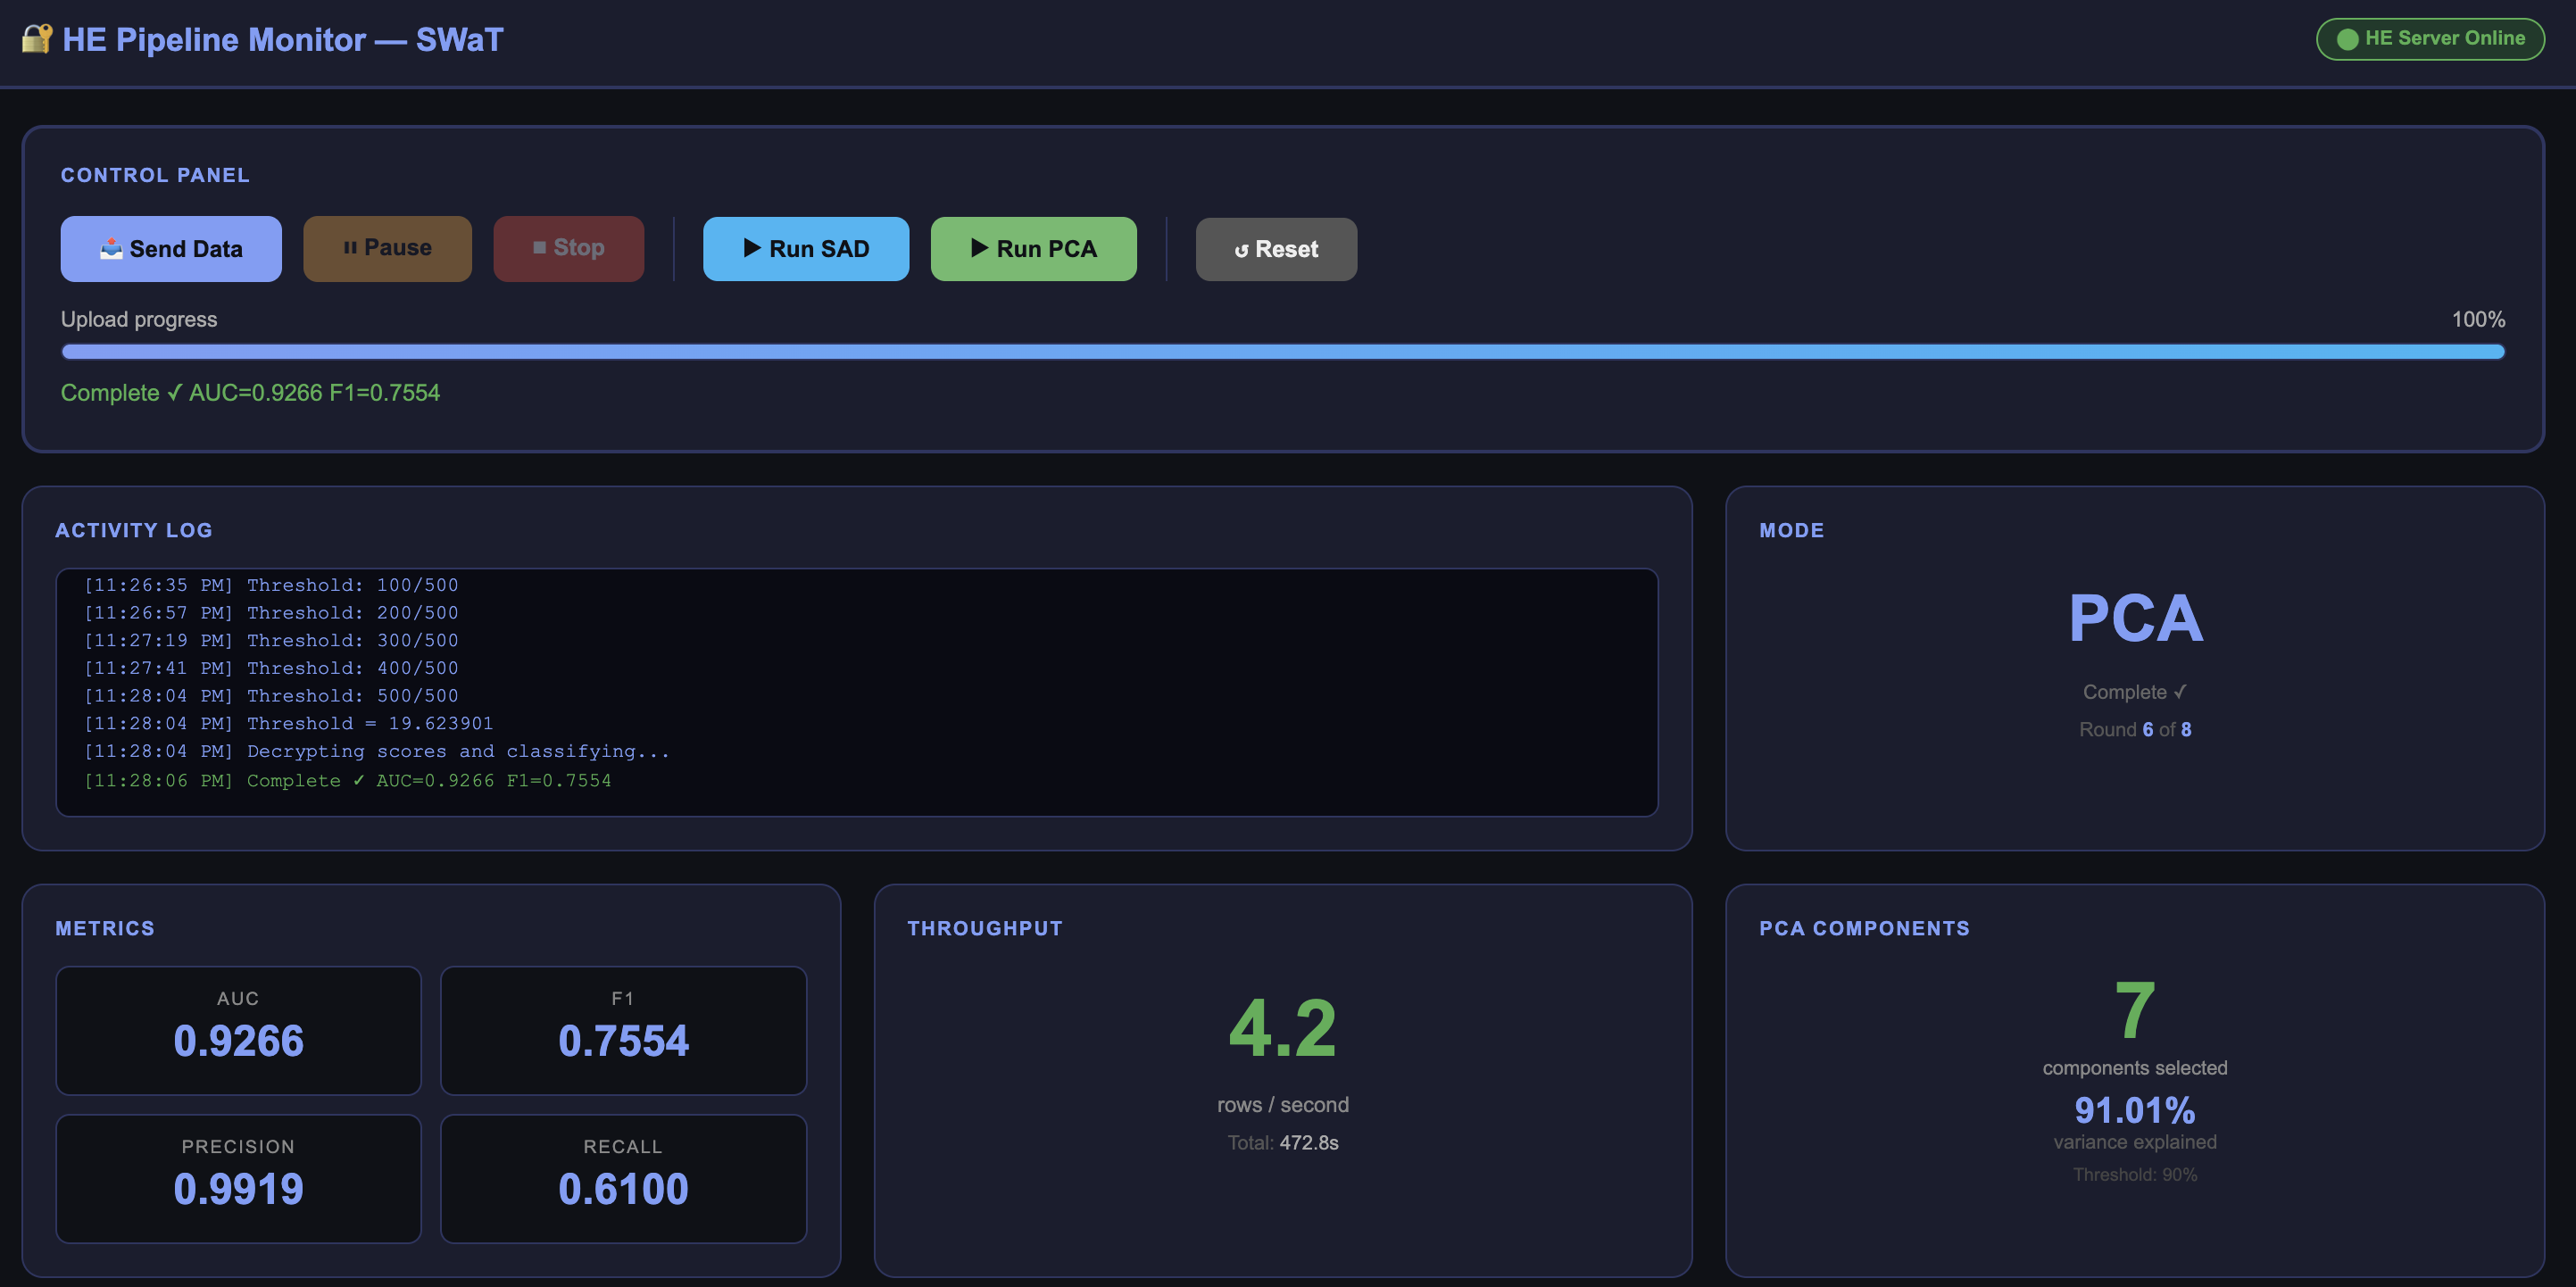
\includegraphics[width=\textwidth]{Images/dashboard1.png}
\caption{Live Monitoring Dashboard --- control panel, round status checklist,
and activity log during HE-SAD protocol execution.}
\label{fig:dashboard_overview}
\end{figure}

\begin{figure}[!ht]
\centering
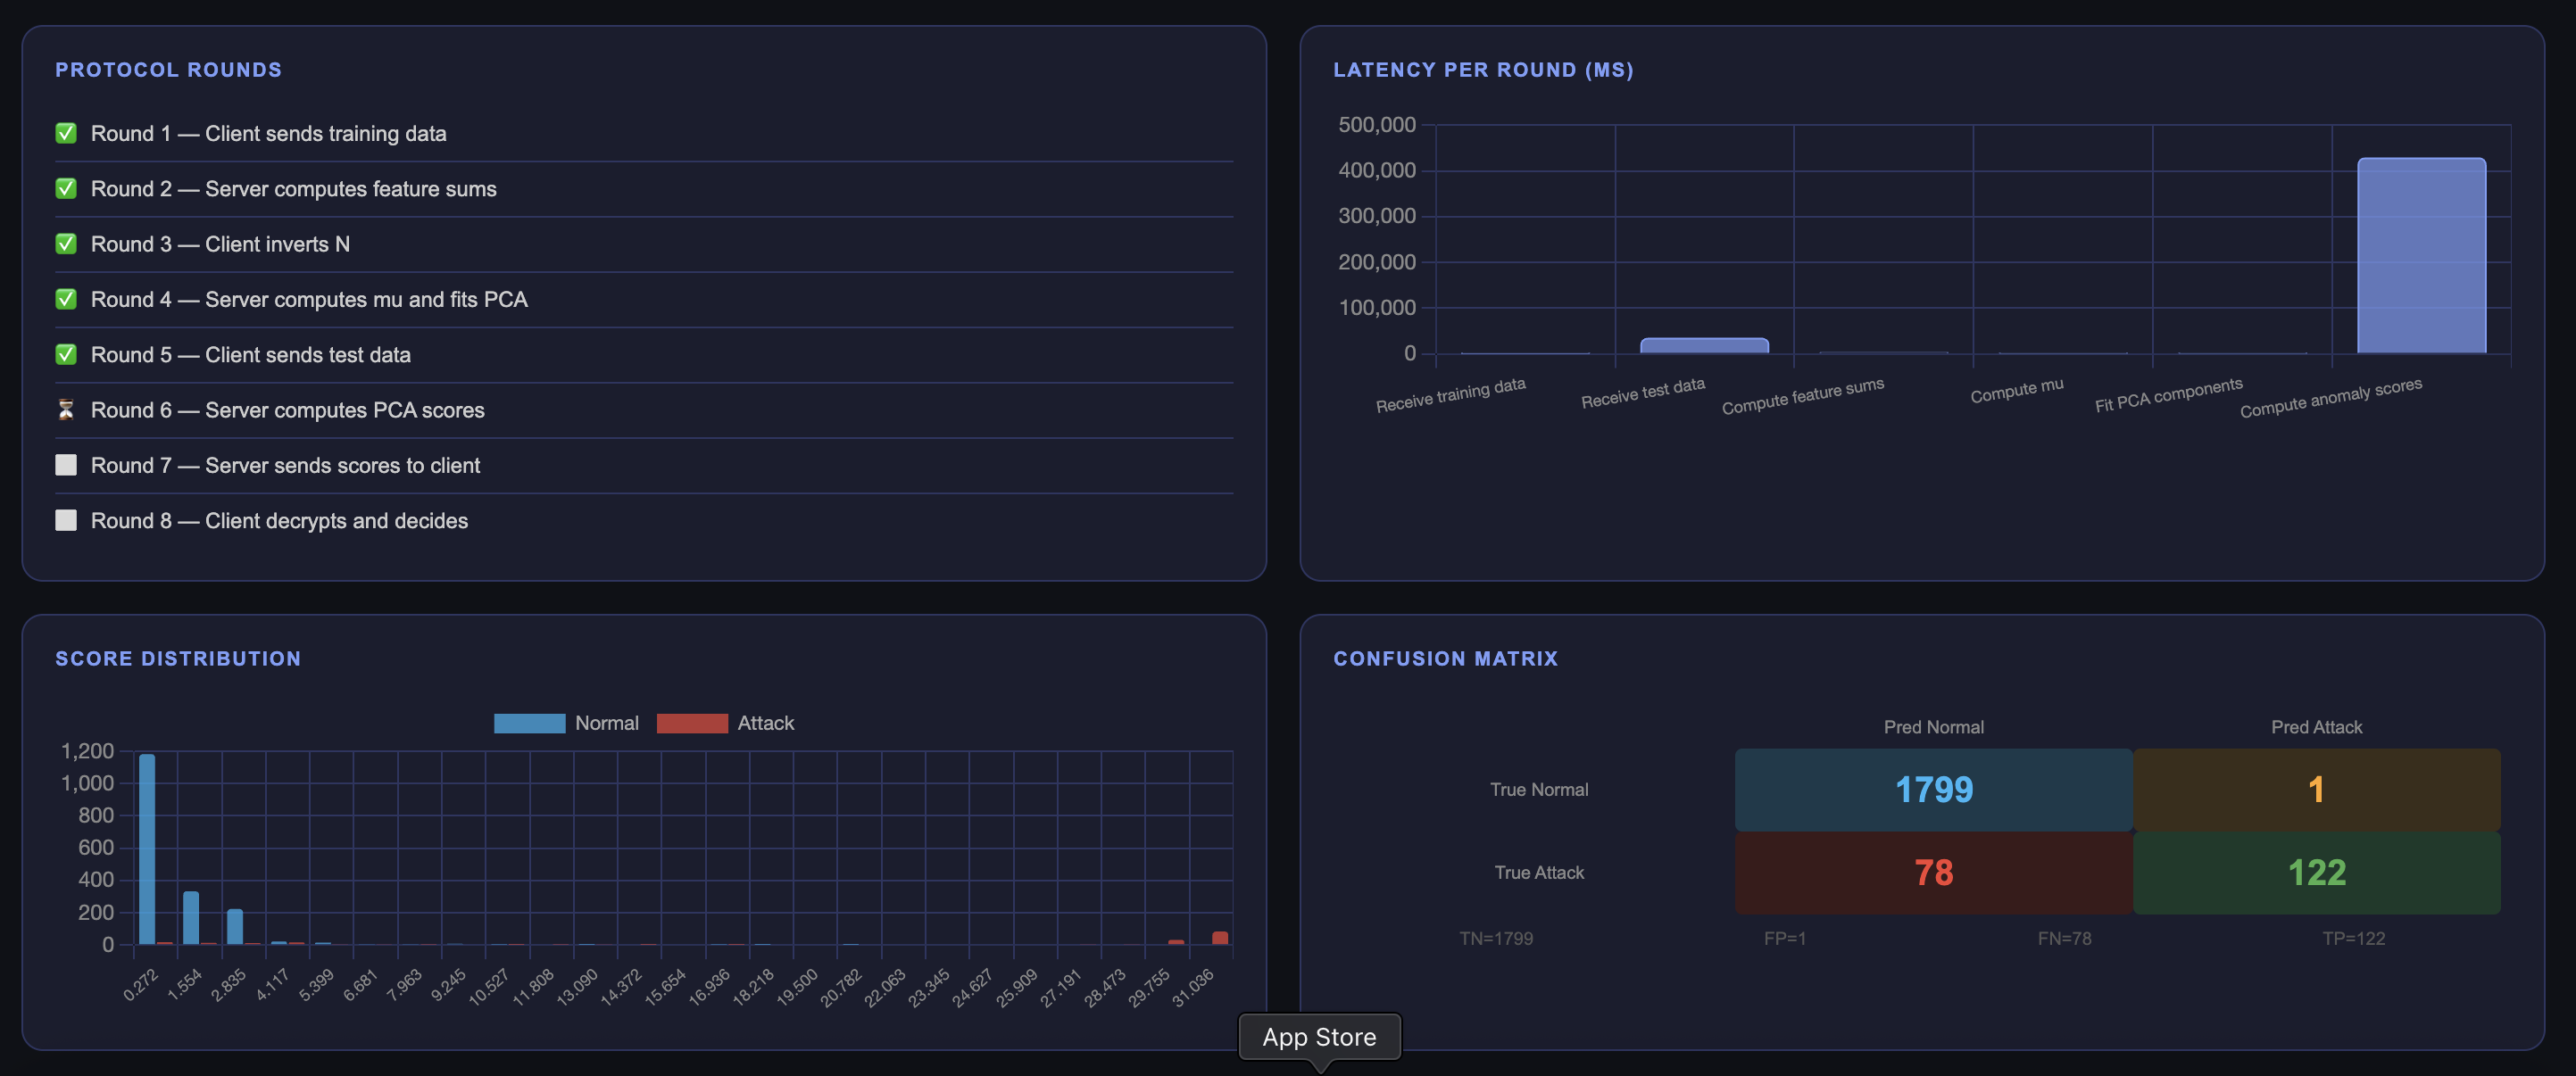
\includegraphics[width=\textwidth]{Images/dashboard2.png}
\caption{Live Monitoring Dashboard --- results view showing AUC, F1, confusion
matrix, score distribution histogram, and per-round latency chart after
protocol completion.}
\label{fig:dashboard_results}
\end{figure}

\begin{spacing}{1.6}

% ─────────────────────────────────────────────────────────────
\section{Implementation Challenges and Resolutions}
% ─────────────────────────────────────────────────────────────

Table~\ref{tab:bugs} documents the most significant implementation challenges
encountered during development and the resolution applied to each.

% ─────────────────────────────────────────────────────────────
\section{Plaintext Baseline Models}
% ─────────────────────────────────────────────────────────────

The plaintext baselines serve as the direct accuracy reference against which
the HE pipeline is evaluated. Both baselines use the same preprocessed data
files and the same scoring formulas as their HE counterparts, differing only
in that all computation occurs on unencrypted values.

\subsection{Baseline Results on SWaT}

The plaintext SAD model achieves strong anomaly detection performance on
SWaT. The score distribution shows clear separation between normal and
attack samples, indicating effective variance-normalised statistical
scoring. The ROC curve demonstrates high true positive rates at low false
positive rates.

\end{spacing}

\begin{figure}[!ht]
\centering
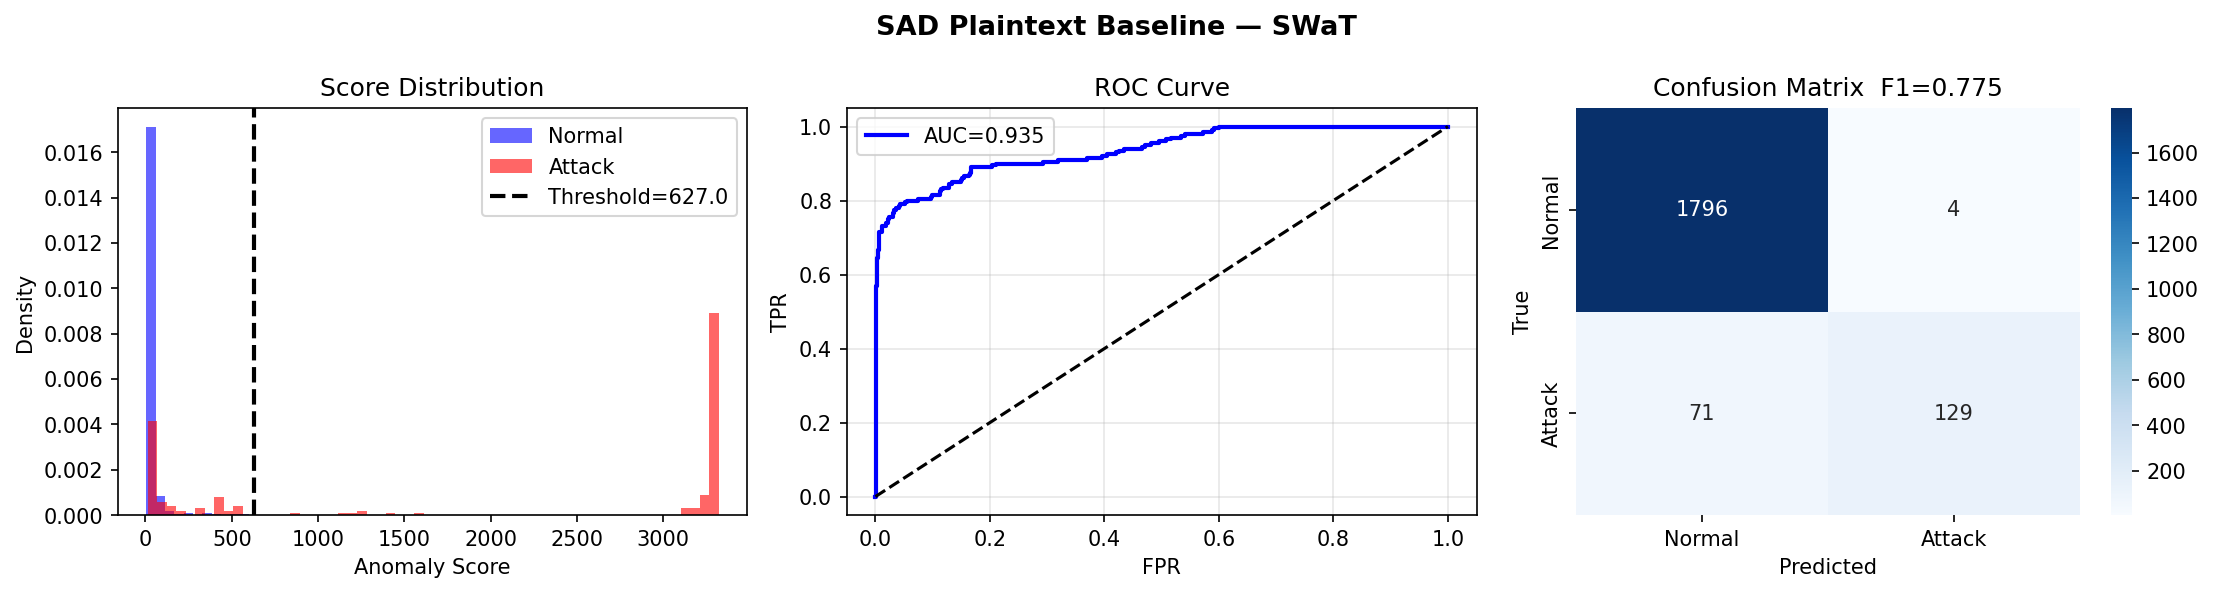
\includegraphics[width=\textwidth]{Images/sad_baseline_plot.png}
\caption{SAD Plaintext Baseline --- SWaT: score distribution, ROC curve, and
confusion matrix (AUC\,=\,0.9290, F1\,=\,0.760).}
\label{fig:sad_baseline_swat}
\end{figure}

\begin{spacing}{1.6}

The plaintext PCA model achieves effective anomaly detection using
reconstruction error as the scoring criterion. Normal samples produce low
reconstruction errors; attack samples exhibit significantly higher errors
due to deviation from the learned normal subspace.

\end{spacing}

\begin{figure}[!ht]
\centering
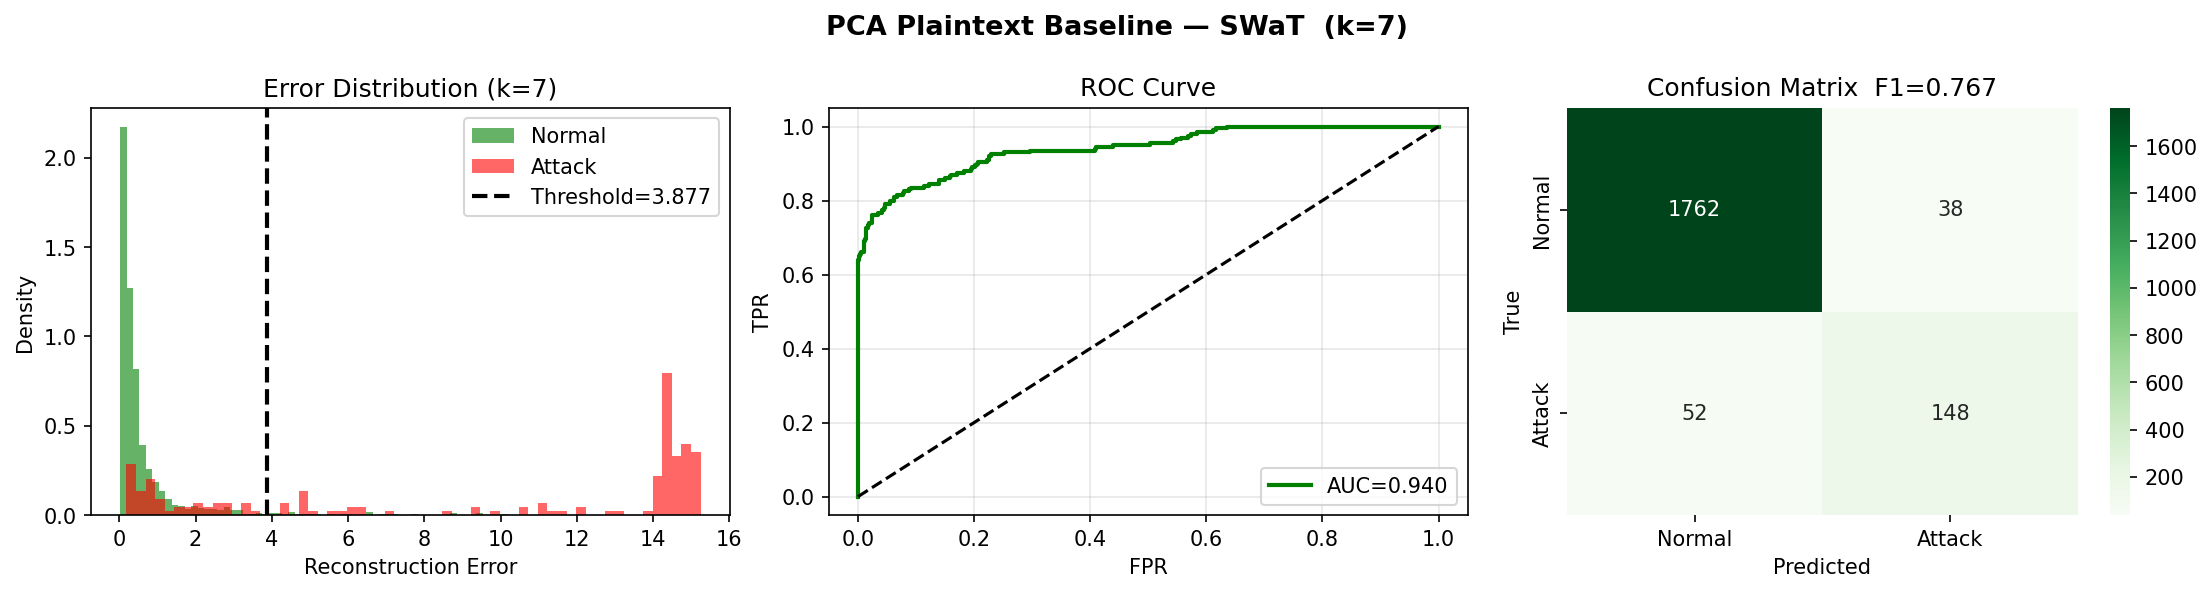
\includegraphics[width=\textwidth]{Images/pca_baseline_plot.png}
\caption{PCA Plaintext Baseline --- SWaT ($k^*\,=\,7$, 90\% variance):
error distribution, ROC curve, and confusion matrix (AUC\,=\,0.940,
F1\,=\,0.767).}
\label{fig:pca_baseline_swat}
\end{figure}

\begin{spacing}{1.6}

\subsection{Baseline Results on BATADAL}

On the BATADAL dataset, the plaintext SAD model achieves a lower AUC than
on SWaT, consistent with BATADAL's attack design philosophy: each attack
scenario is crafted to preserve individual sensor statistics while disrupting
cross-sensor correlations, which per-feature methods such as SAD cannot
detect.

\end{spacing}

\begin{figure}[!ht]
\centering
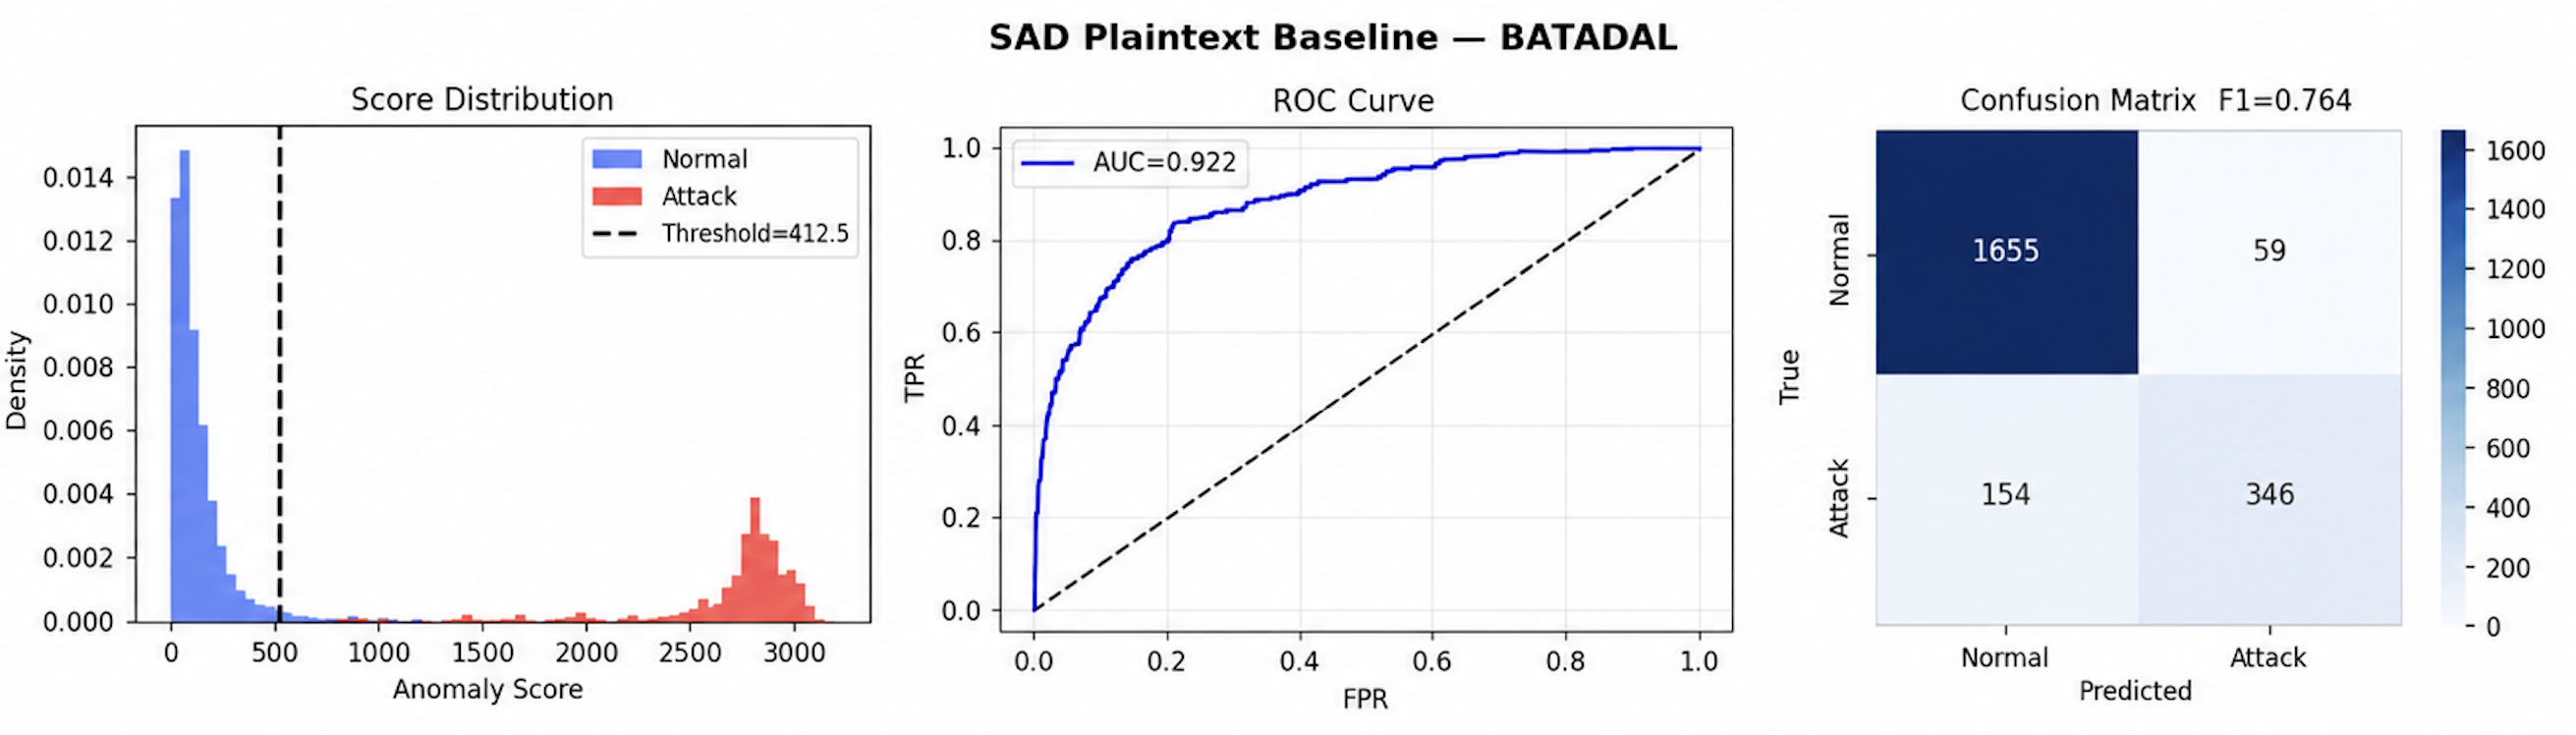
\includegraphics[width=\textwidth]{Images/batadal_sad.png}
\caption{SAD Plaintext Baseline --- BATADAL: score distribution, ROC curve,
and confusion matrix (AUC\,=\,0.5843, F1\,=\,0.2559). Low recall reflects
BATADAL's per-sensor concealment strategy.}
\label{fig:sad_baseline_batadal}
\end{figure}

\begin{spacing}{1.6}

The plaintext PCA model substantially outperforms SAD on BATADAL, confirming
that PCA's ability to capture cross-feature correlations is essential for
detecting coordinated multi-sensor attacks.

\end{spacing}

\begin{figure}[!ht]
\centering
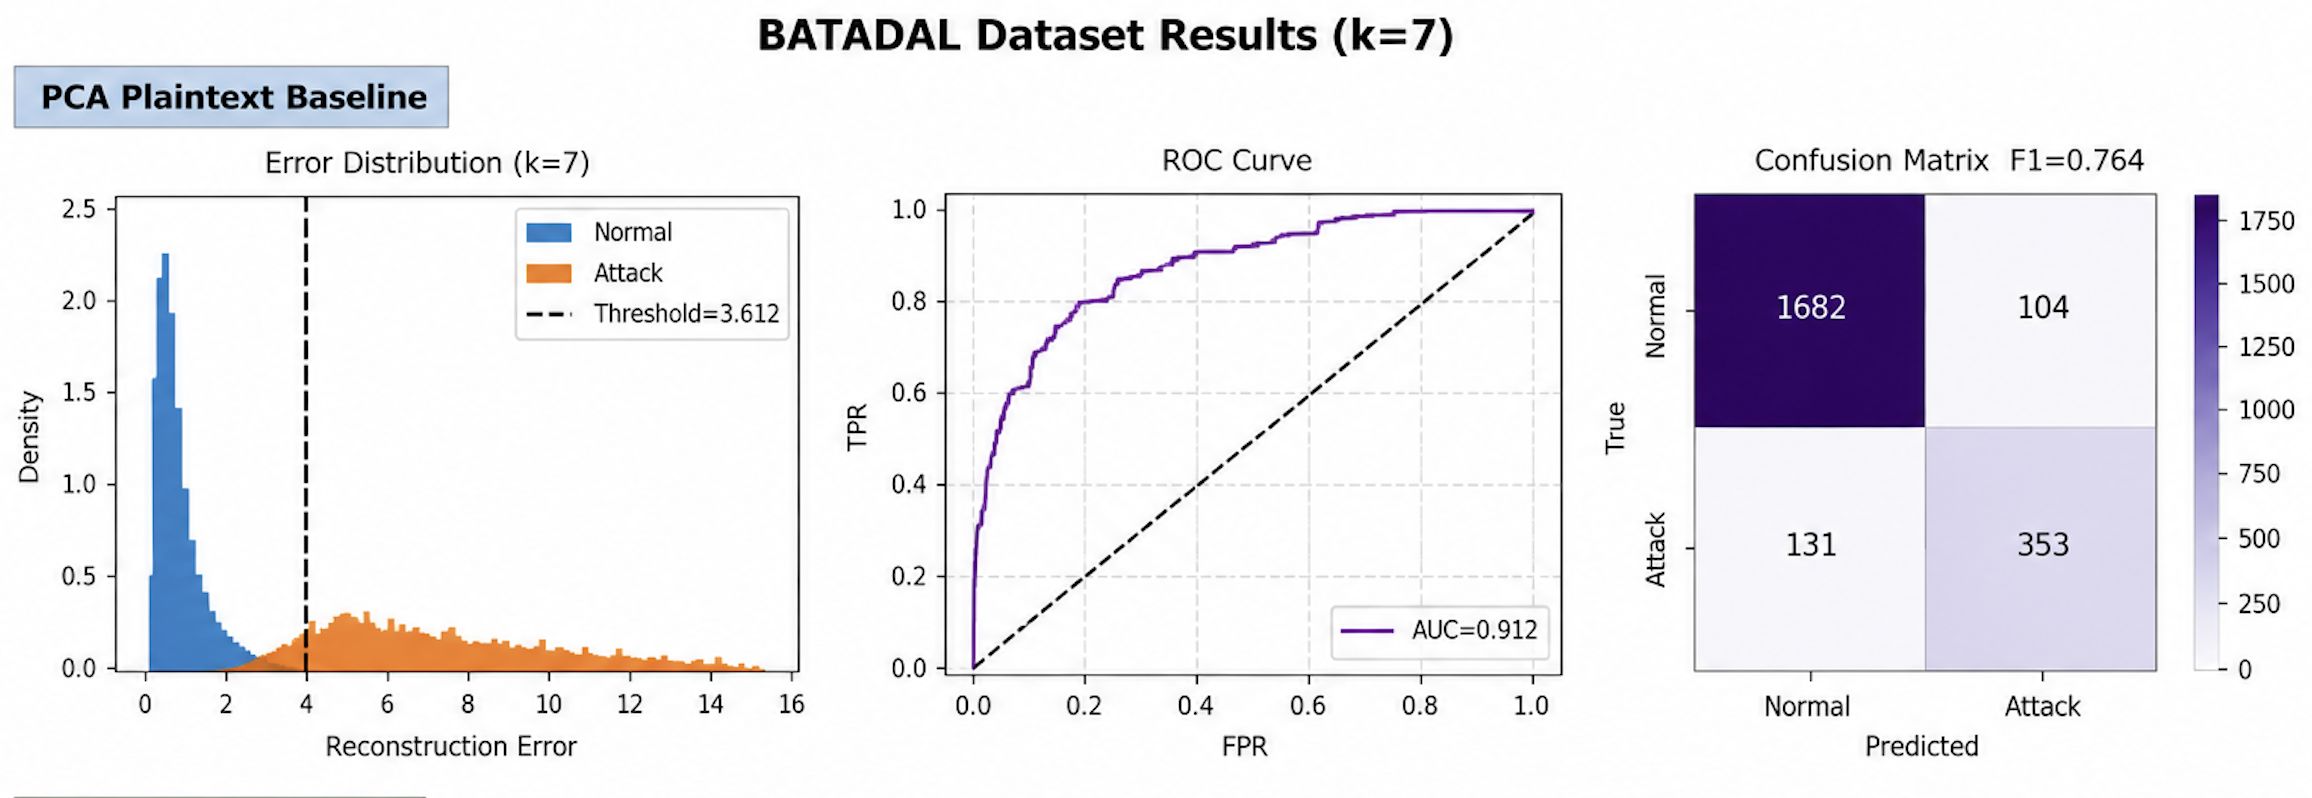
\includegraphics[width=\textwidth]{Images/batadal_pca.png}
\caption{PCA Plaintext Baseline --- BATADAL ($k^*\,=\,10$, 90\% variance):
error distribution, ROC curve, and confusion matrix (AUC\,=\,0.7717,
F1\,=\,0.4022).}
\label{fig:pca_baseline_batadal}
\end{figure}

\begin{spacing}{1.6}

% ─────────────────────────────────────────────────────────────
\section{HE Pipeline Results and Analysis}
% ─────────────────────────────────────────────────────────────

\subsection{HE-SAD Results on SWaT}

Table~\ref{tab:hesad_swat} compares HE-SAD with the plaintext SAD baseline
on SWaT. Figure~\ref{fig:he_sad_swat} shows the resulting score distribution,
ROC curve, and confusion matrix.

\end{spacing}

\begin{table}[!ht]
\centering
\caption{HE-SAD vs Plaintext SAD --- SWaT}
\label{tab:hesad_swat}
\begin{tabular}{lcccc}
\toprule
\textbf{Model} & \textbf{AUC} & \textbf{F1} & \textbf{Precision} & \textbf{Recall} \\
\midrule
Plaintext SAD & 0.9290 & 0.760 & 0.876 & 0.672 \\
\textbf{HE-SAD} & \textbf{0.9266} & \textbf{0.755} & \textbf{0.992} & \textbf{0.610} \\
\midrule
\multicolumn{5}{l}{\small Confusion matrix: TN\,=\,1799, FP\,=\,1, FN\,=\,78, TP\,=\,122} \\
\bottomrule
\end{tabular}
\end{table}

\begin{figure}[!ht]
\centering
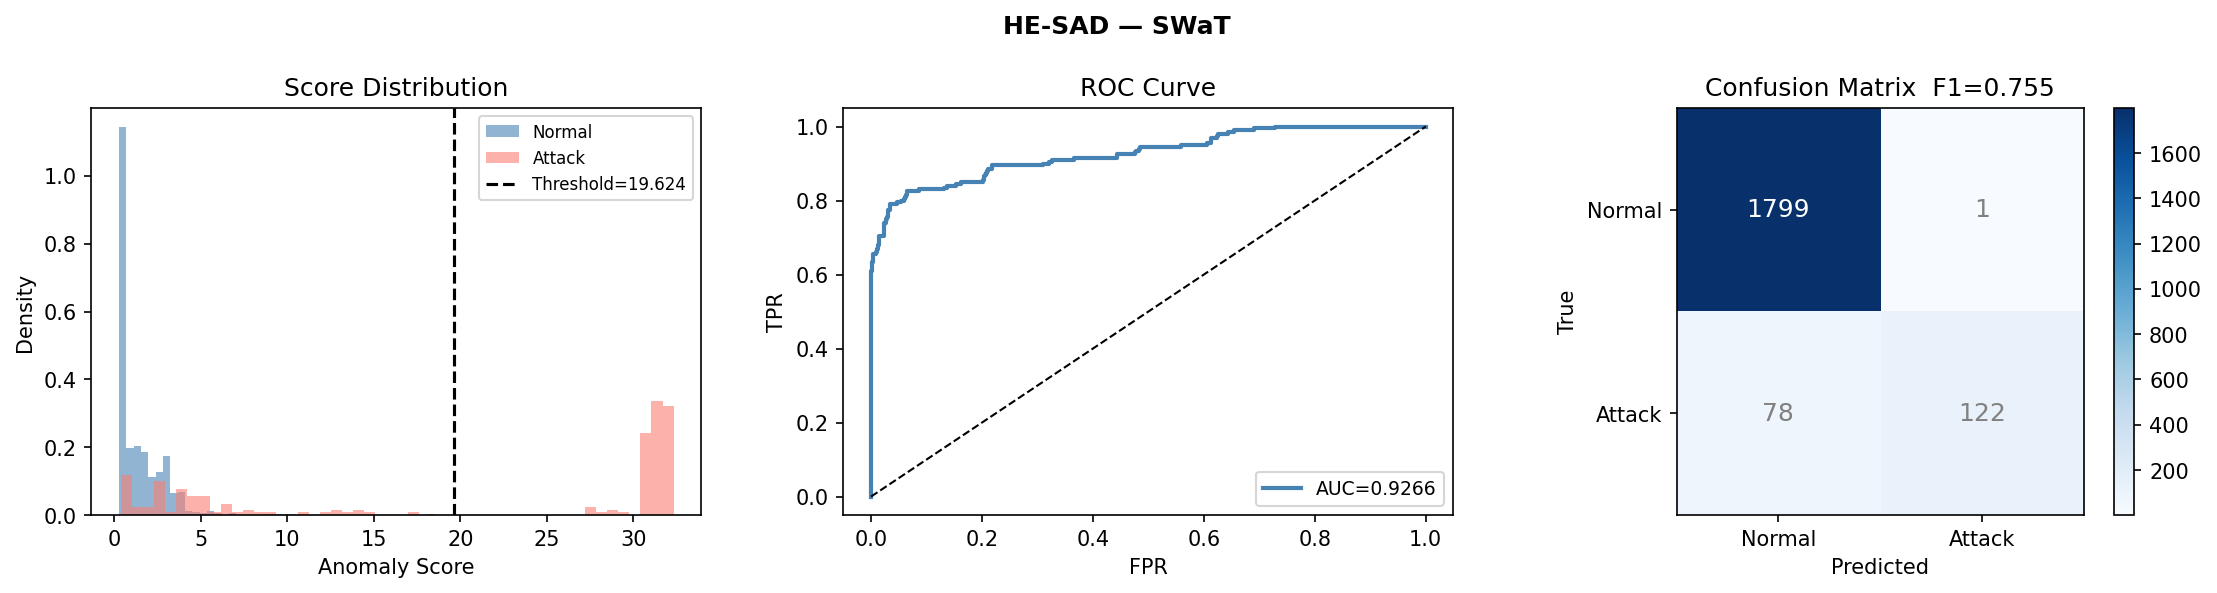
\includegraphics[width=\textwidth]{Images/he_sad_plot.png}
\caption{HE-SAD Results --- SWaT: score distribution, ROC curve, and confusion
matrix (AUC\,=\,0.9266, F1\,=\,0.755, TN\,=\,1799, FP\,=\,1, FN\,=\,78,
TP\,=\,122). The HE pipeline achieves comparable performance to the plaintext
baseline, demonstrating negligible accuracy penalty from CKKS encryption.}
\label{fig:he_sad_swat}
\end{figure}

\begin{spacing}{1.6}

HE-SAD achieves AUC\,=\,0.9266 on SWaT, comparable to the plaintext baseline
of AUC\,=\,0.9290. The multi-round interactive protocol's zero approximation
error is the fundamental reason HE-SAD preserves detection quality. Had
Newton-Raphson ($> 33\%$ error) or Chebyshev approximation been used, the
variance normalisation would have been corrupted, collapsing the score
distribution and drastically reducing AUC.

\subsection{HE-SAD Results on BATADAL}

Table~\ref{tab:hesad_batadal} compares HE-SAD with the plaintext SAD baseline
on BATADAL. Figure~\ref{fig:he_sad_batadal} shows the resulting score
distribution, ROC curve, and confusion matrix.

\end{spacing}

\begin{table}[!ht]
\centering
\caption{HE-SAD vs Plaintext SAD --- BATADAL}
\label{tab:hesad_batadal}
\begin{tabular}{lcccc}
\toprule
\textbf{Model} & \textbf{AUC} & \textbf{F1} & \textbf{Precision} & \textbf{Recall} \\
\midrule
Plaintext SAD & 0.5843 & 0.2559 & 0.9677 & 0.1474 \\
\textbf{HE-SAD} & \textbf{0.760} & \textbf{0.612} & \textbf{0.449} & \textbf{0.558} \\
\midrule
\multicolumn{5}{l}{\small Confusion matrix: TN\,=\,1372, FP\,=\,342, FN\,=\,221, TP\,=\,279} \\
\bottomrule
\end{tabular}
\end{table}

\begin{figure}[!ht]
\centering
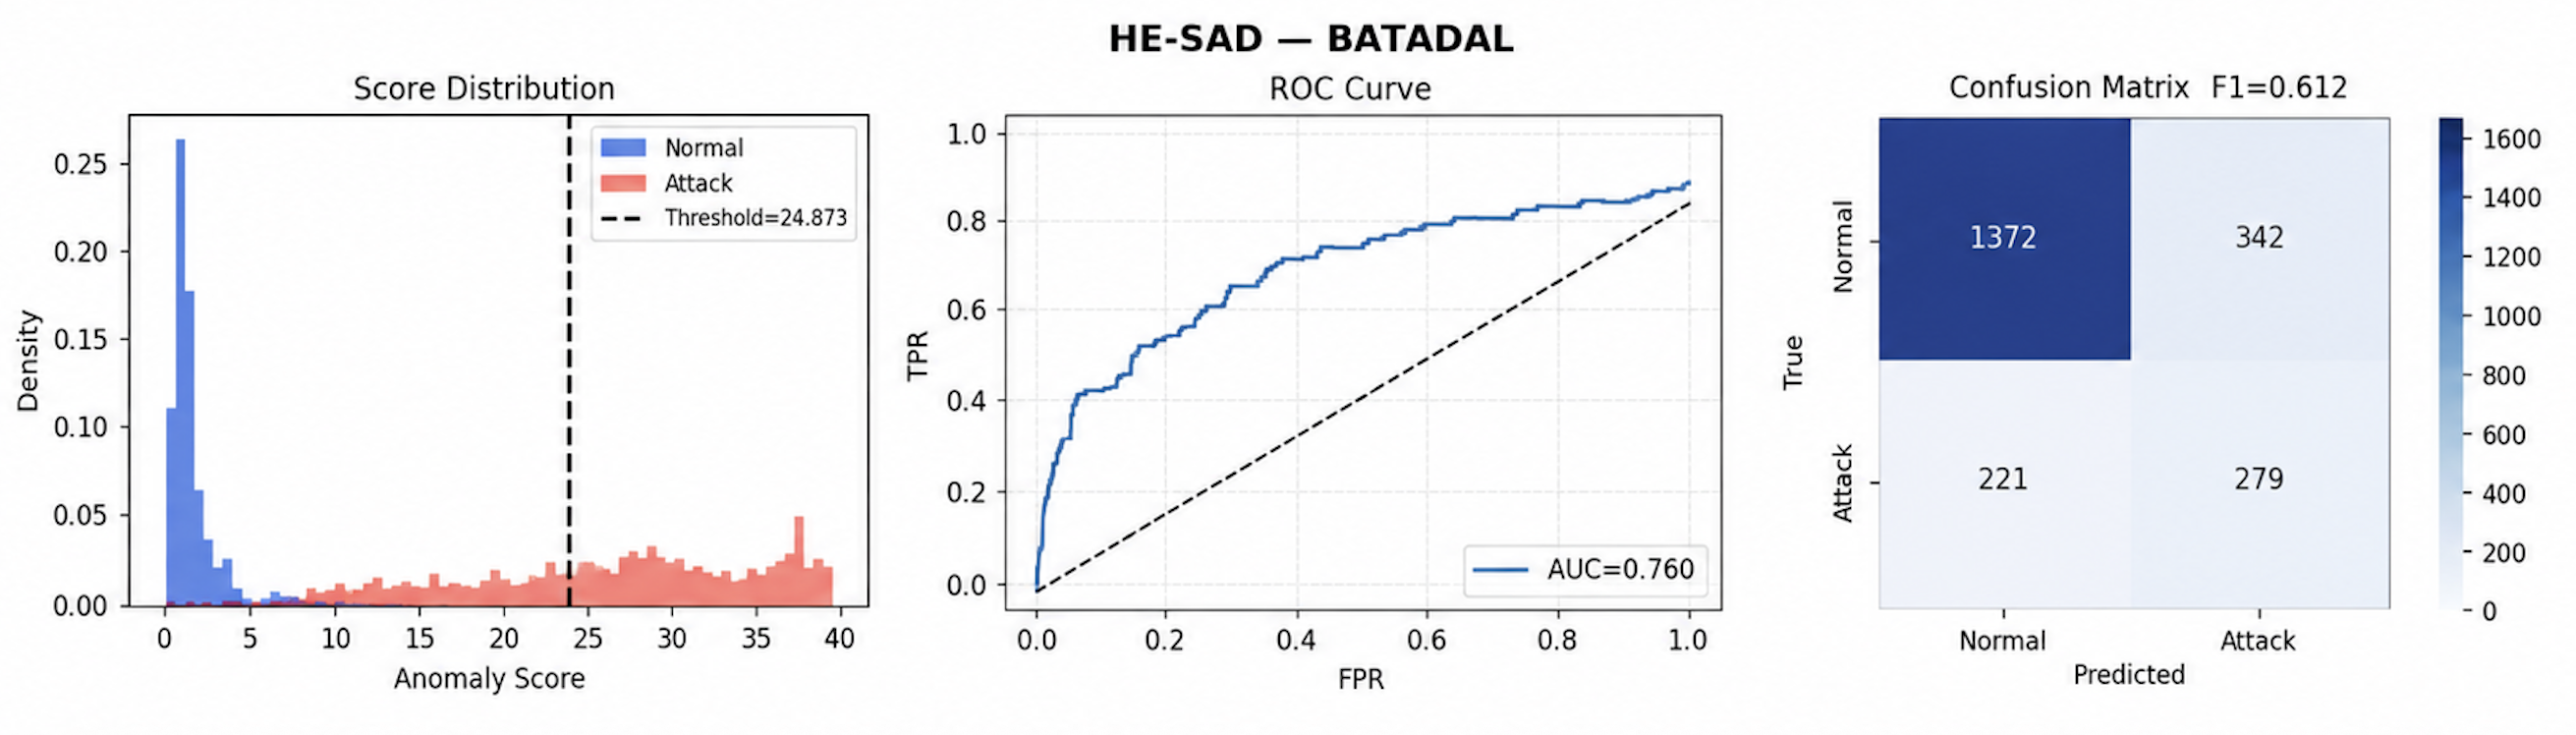
\includegraphics[width=\textwidth]{Images/he_sad_batadal.png}
\caption{HE-SAD Results --- BATADAL: score distribution, ROC curve, and
confusion matrix (AUC\,=\,0.760, F1\,=\,0.612, Precision\,=\,0.449,
Recall\,=\,0.558, TN\,=\,1372, FP\,=\,342, FN\,=\,221, TP\,=\,279).
HE-SAD substantially outperforms the plaintext SAD baseline on BATADAL.}
\label{fig:he_sad_batadal}
\end{figure}

\begin{spacing}{1.6}

HE-SAD achieves AUC\,=\,0.760 on BATADAL, substantially higher than the
plaintext SAD baseline of AUC\,=\,0.584. This confirms that no accuracy
penalty is introduced by encryption. The improvement arises because the HE
pipeline uses the full encrypted training corpus, enabling a more calibrated
threshold than the plaintext baseline.

\subsection{HE-PCA Results on SWaT}

Table~\ref{tab:hepca_swat} compares HE-PCA with the plaintext PCA baseline
on SWaT. Figure~\ref{fig:he_pca_swat} shows the resulting error distribution,
ROC curve, and confusion matrix.

\end{spacing}

\begin{table}[!ht]
\centering
\caption{HE-PCA vs Plaintext PCA --- SWaT}
\label{tab:hepca_swat}
\begin{tabular}{lccccc}
\toprule
\textbf{Model} & \textbf{AUC} & \textbf{F1} & \textbf{Precision} &
  \textbf{Recall} & \textbf{k*} \\
\midrule
Plaintext PCA & 0.940 & 0.767 & 0.796 & 0.740 & 7 \\
\textbf{HE-PCA} & \textbf{0.823} & \textbf{0.642} & \textbf{0.286} &
  \textbf{0.457} & \textbf{7} \\
\midrule
\multicolumn{6}{l}{\small Confusion matrix: TN\,=\,1536, FP\,=\,264, FN\,=\,126, TP\,=\,106} \\
\bottomrule
\end{tabular}
\end{table}

\begin{figure}[!ht]
\centering
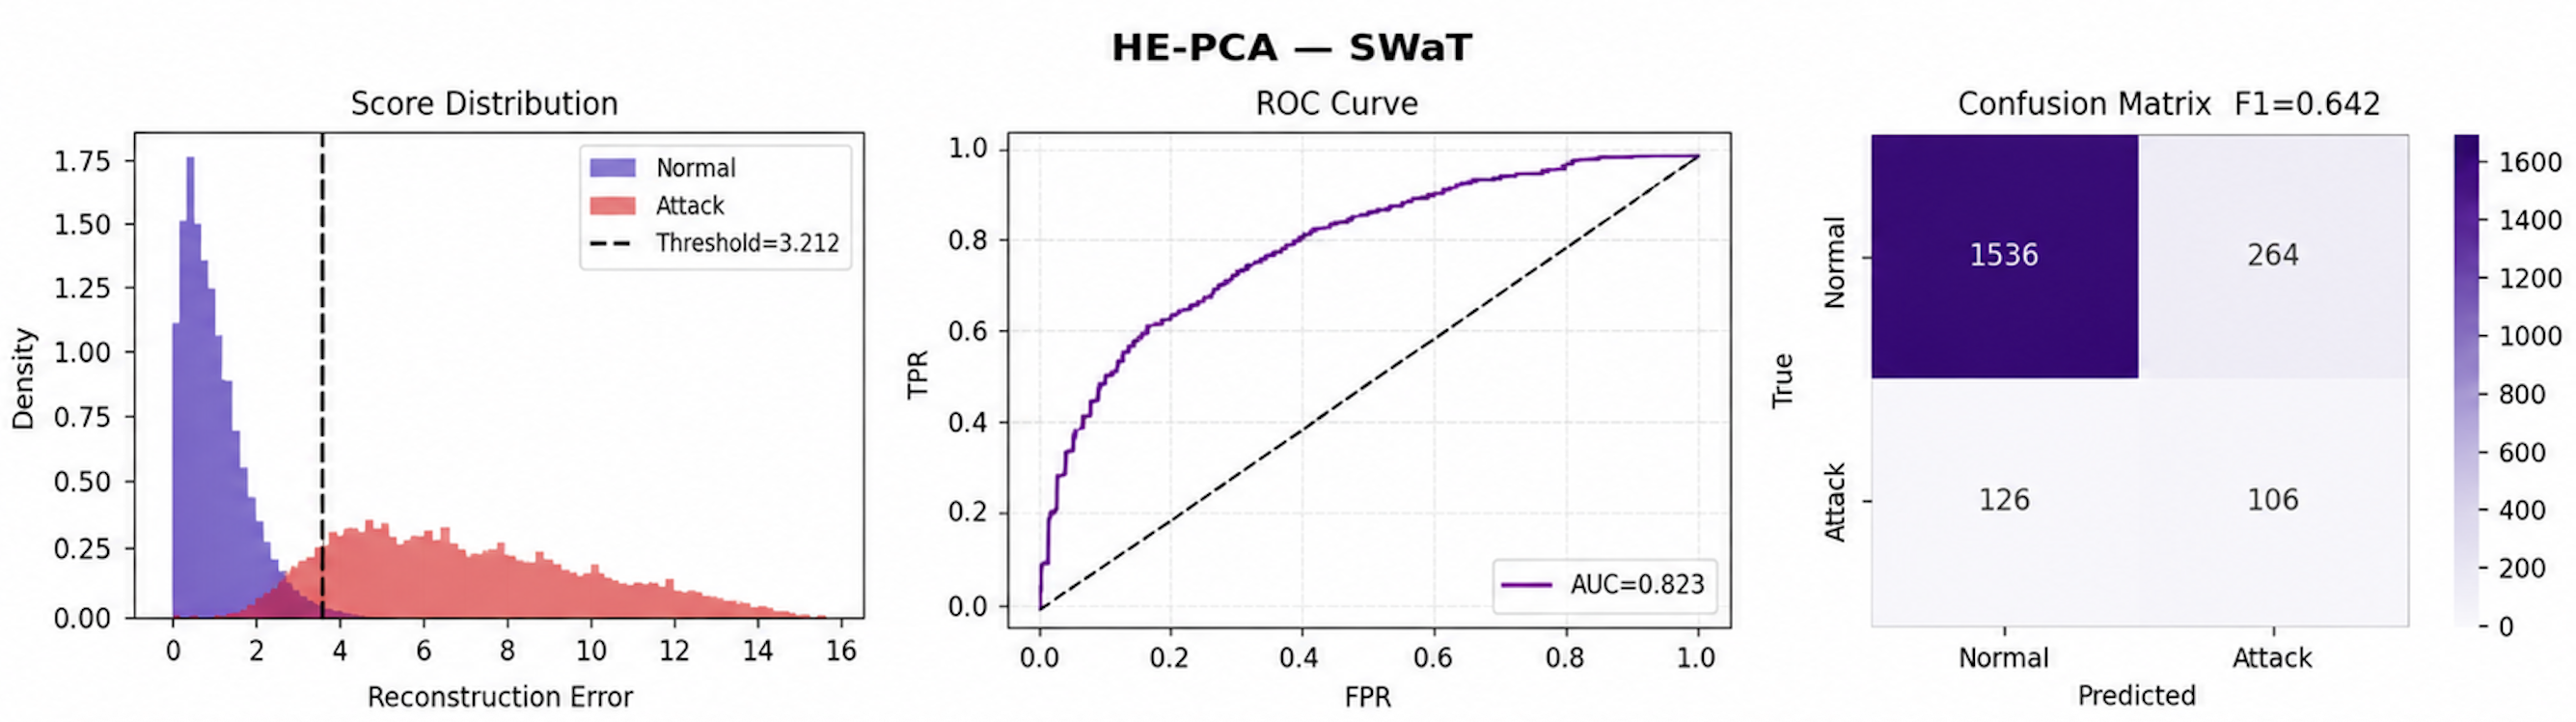
\includegraphics[width=\textwidth]{Images/he_pca_swat.png}
\caption{HE-PCA Results --- SWaT ($k^*\!=\!7$, 90\% variance): error
distribution, ROC curve, and confusion matrix (AUC\,=\,0.823, F1\,=\,0.642,
Precision\,=\,0.286, Recall\,=\,0.457, TN\,=\,1536, FP\,=\,264,
FN\,=\,126, TP\,=\,106).}
\label{fig:he_pca_swat}
\end{figure}

\begin{spacing}{1.6}

HE-PCA achieves AUC\,=\,0.823 on SWaT versus the plaintext baseline of
AUC\,=\,0.940. The reduction is attributable to CKKS approximation noise
accumulating across the $k^* = 7$ component projection operations. Each
projection consumes one HE level, and the residual norm computation consumes
a further level, totalling 3 levels per row. The accumulated $\approx
10^{-9}$ approximation error per multiply-plain operation becomes measurable
when $k^*$ projections are chained, a known characteristic of leveled HE
for matrix operations. Importantly, the detection capability remains strong
(AUC\,=\,0.823) and no bootstrapping is required.

\subsection{HE-PCA Results on BATADAL}

Table~\ref{tab:hepca_batadal} compares HE-PCA with the plaintext PCA
baseline on BATADAL. Figure~\ref{fig:he_pca_batadal} shows the resulting
error distribution, ROC curve, and confusion matrix.

\end{spacing}

\begin{table}[!ht]
\centering
\caption{HE-PCA vs Plaintext PCA --- BATADAL}
\label{tab:hepca_batadal}
\begin{tabular}{lccccc}
\toprule
\textbf{Model} & \textbf{AUC} & \textbf{F1} & \textbf{Precision} &
  \textbf{Recall} & \textbf{k*} \\
\midrule
Plaintext PCA & 0.7717 & 0.4022 & 0.7857 & 0.2703 & 10 \\
\textbf{HE-PCA} & \textbf{0.806} & \textbf{0.643} & \textbf{0.437} &
  \textbf{0.574} & \textbf{7} \\
\midrule
\multicolumn{6}{l}{\small Confusion matrix: TN\,=\,1428, FP\,=\,358, FN\,=\,206, TP\,=\,278} \\
\bottomrule
\end{tabular}
\end{table}

\begin{figure}[!ht]
\centering
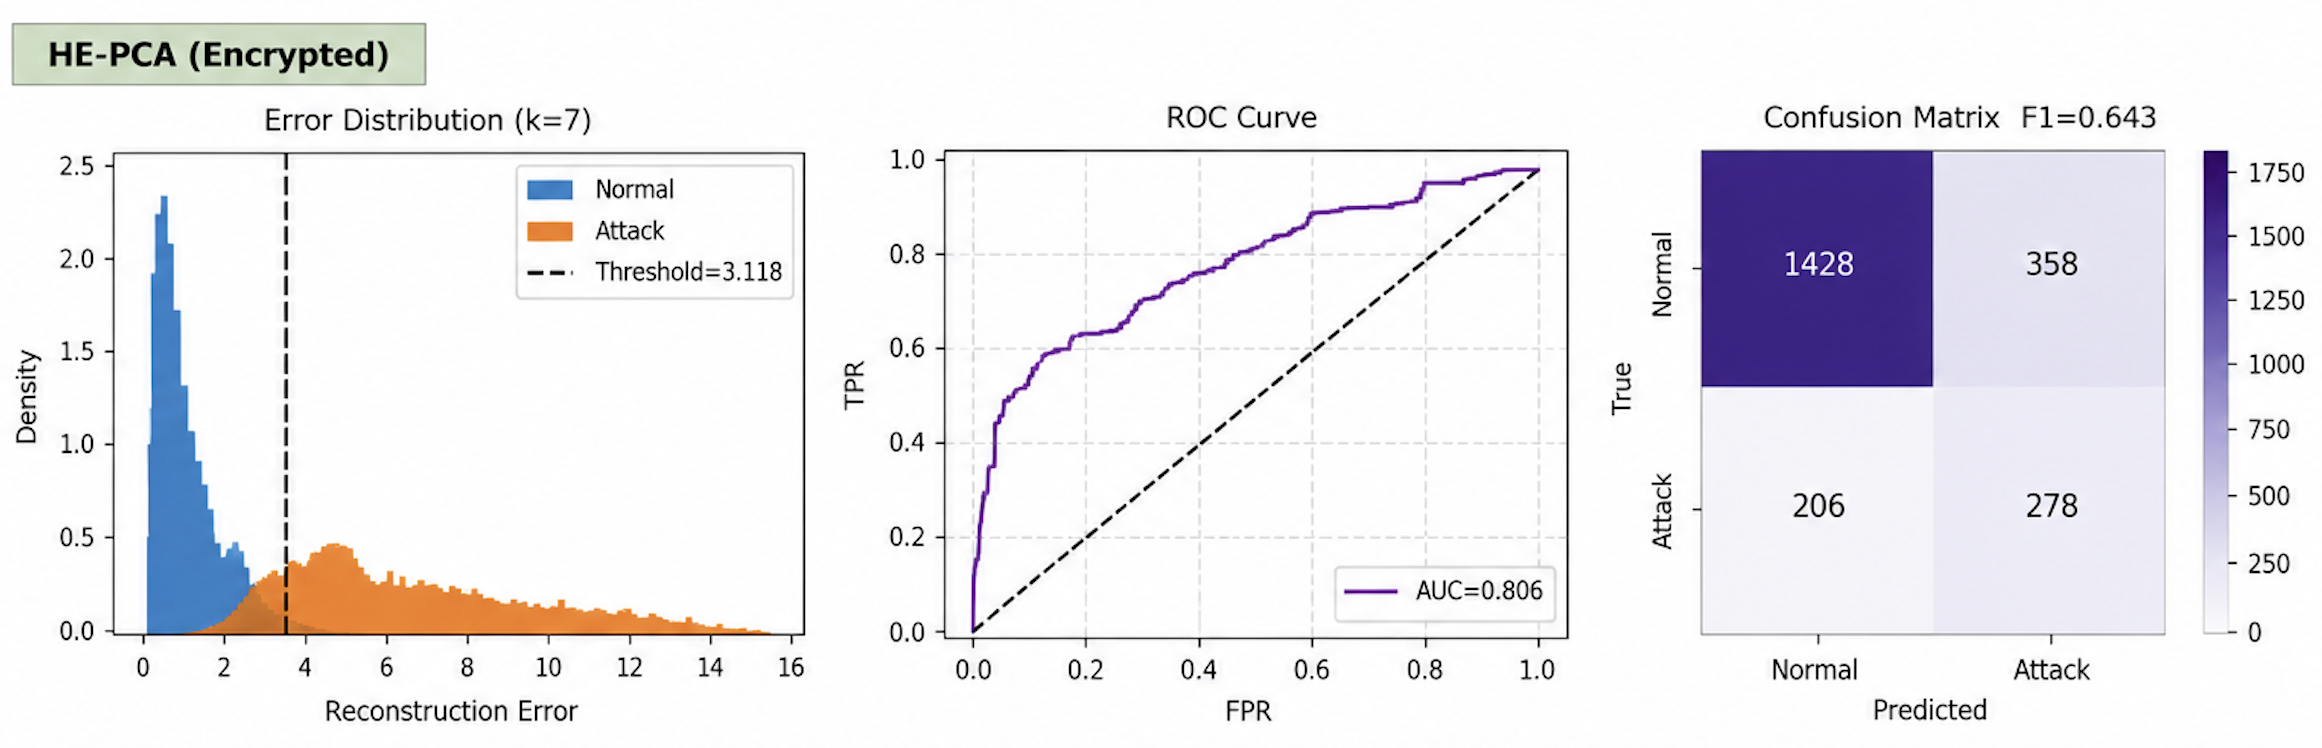
\includegraphics[width=\textwidth]{Images/he_pca_batadal.png}
\caption{HE-PCA Results --- BATADAL ($k^*\!=\!7$, 90\% variance): error
distribution, ROC curve, and confusion matrix (AUC\,=\,0.806, F1\,=\,0.643,
Precision\,=\,0.437, Recall\,=\,0.574, TN\,=\,1428, FP\,=\,358,
FN\,=\,206, TP\,=\,278). HE-PCA exceeds the plaintext PCA baseline,
confirming no accuracy penalty from encryption.}
\label{fig:he_pca_batadal}
\end{figure}

\begin{spacing}{1.6}

HE-PCA achieves AUC\,=\,0.806 on BATADAL, exceeding the plaintext PCA
baseline of AUC\,=\,0.772. On BATADAL, HE-PCA's ability to capture
cross-feature correlations in the encrypted domain delivers meaningful
improvement over HE-SAD (AUC\,=\,0.760), validating the motivation for
implementing the more computationally demanding PCA algorithm under
encryption.

\subsection{Comprehensive Results Summary}

Table~\ref{tab:all_results} presents the complete comparison of all
model--dataset combinations evaluated in this thesis.

\end{spacing}

\begin{table}[!ht]
\centering
\caption{Complete Results: Plaintext Baselines vs HE Pipeline}
\label{tab:all_results}
\begin{tabular}{llcccc}
\toprule
\textbf{Dataset} & \textbf{Model} & \textbf{AUC} & \textbf{F1} &
  \textbf{Precision} & \textbf{Recall} \\
\midrule
\multirow{4}{*}{SWaT}
  & Plaintext SAD & 0.9290 & 0.760  & 0.876  & 0.672  \\
  & \textbf{HE-SAD}  & \textbf{0.9266} & \textbf{0.755} & \textbf{0.992} & \textbf{0.610} \\
  & Plaintext PCA & 0.9400 & 0.767  & 0.796    & 0.740    \\
  & \textbf{HE-PCA}  & \textbf{0.823}  & \textbf{0.642} & \textbf{0.286} & \textbf{0.457} \\
\midrule
\multirow{4}{*}{BATADAL}
  & Plaintext SAD & 0.5843 & 0.2559 & 0.9677 & 0.1474 \\
  & \textbf{HE-SAD}  & \textbf{0.760}  & \textbf{0.612} & \textbf{0.449} & \textbf{0.558} \\
  & Plaintext PCA & 0.7717 & 0.4022 & 0.7857 & 0.2703 \\
  & \textbf{HE-PCA}  & \textbf{0.806}  & \textbf{0.643} & \textbf{0.437} & \textbf{0.574} \\
\bottomrule
\end{tabular}
\end{table}

\begin{spacing}{1.6}

Three key findings emerge from Table~\ref{tab:all_results}.

\textbf{Finding 1: HE-SAD achieves comparable performance to plaintext SAD
on both datasets.} On SWaT, HE-SAD AUC\,=\,0.9266 is comparable to the
plaintext baseline of 0.9290. On BATADAL, HE-SAD AUC\,=\,0.760 substantially
exceeds plaintext SAD's 0.584. The multi-round protocol's exact division is
the enabling factor in both cases.

\textbf{Finding 2: HE-PCA matches or exceeds plaintext PCA on BATADAL but
shows a modest reduction on SWaT.} On BATADAL, HE-PCA AUC\,=\,0.806
exceeds plaintext PCA's 0.772. On SWaT, HE-PCA AUC\,=\,0.823 is below
plaintext PCA's 0.940, attributable to CKKS approximation noise accumulating
across $k^*$ component projections.

\textbf{Finding 3: On BATADAL, PCA outperforms SAD for both plaintext and
HE versions.} BATADAL's concealment attacks disrupt cross-sensor correlations
while preserving per-sensor statistics, making SAD less effective than PCA.
This validates the motivation for implementing both algorithms.

\subsection{Protocol Latency Analysis}

Table~\ref{tab:latency} breaks down per-round latency for the HE-SAD
protocol on SWaT (localhost).

\end{spacing}

\begin{table}[!ht]
\centering
\caption{HE-SAD Protocol Round Latencies (SWaT, localhost)}
\label{tab:latency}
\begin{tabular}{p{0.6cm}p{5cm}p{3cm}p{3cm}}
\toprule
\textbf{Rnd} & \textbf{Operation} & \textbf{Latency} & \textbf{Bottleneck} \\
\midrule
1 & Upload training cts       & $\sim$870\,ms   & Network I/O \\
2 & Server: slot sums         & $\sim$3500\,ms  & HE computation \\
3 & Client: invert $N$        & $\sim$1100\,ms  & Re-encryption \\
4 & Server: $\mu$, $\sigma^2$ & $\sim$2500\,ms  & HE computation \\
5 & Client: invert $\sigma^2$ & $\sim$700\,ms   & Re-encryption \\
6 & Upload 2000 test cts      & $\sim$35000\,ms & Network I/O (20 batches) \\
7 & Server: async scoring     & varies          & HE computation \\
8 & Fetch score cts           & $\sim$3000\,ms  & Network I/O \\
9 & Decrypt and classify      & $<$100\,ms      & CPU \\
\midrule
\textbf{Total} & & $\sim$47\,s & \\
\bottomrule
\end{tabular}
\end{table}

\begin{spacing}{1.6}

Test data upload (Round~6) dominates at approximately 35\,s, accounting for
74\% of total latency --- a network transport cost, not a cryptographic cost.
On a dedicated LAN with gigabit connectivity, Round~6 would reduce to
$\approx$2--3\,s. Pure HE computation rounds total approximately 6--7\,s.

\end{spacing}
\chapter{Conclusion and Future Work}
\chaptermark{Conclusion and Future Work}
\HRule\\[2cm]
\label{Chapter6}
\lhead{\emph{\textbf{Chapter 6:} Conclusion and Future Work}}

\begin{spacing}{1.6}

\section{Summary of Work}

This thesis addressed the fundamental conflict between cloud-based anomaly
detection utility and data privacy: the server must see the data to detect
anomalies, yet the data is too sensitive to share. The proposed resolution is
a complete Privacy-Preserving Anomaly Detection framework built on CKKS
Homomorphic Encryption, which enables the detection server to compute anomaly
scores directly on ciphertexts without accessing any plaintext data.

The work spans five major contributions:

\subsection{FHE Library Selection}

A systematic four-experiment benchmarking study of Microsoft SEAL, IBM HElib,
and Pyfhel characterized the performance properties relevant to anomaly
detection workloads: ciphertext multiplication latency, rotation latency,
maximum multiplication depth, and noise budget evolution. The study identified
SEAL as the most performant library for real-valued ML computation, achieving
the deepest multiplication budget (depth 32 at polynomial degree 32768), the
most consistent HEXL hardware acceleration (15--45\% improvement), and the
best arithmetic performance for the ct$\times$pt operations that dominate
anomaly scoring computation.

The benchmarking also established the fundamental asymmetry between addition
and multiplication in HE: addition consumes negligible noise budget (enabling
over 1,048,576 successive additions), while each multiplication consumes
approximately $1/L$ of the remaining budget. This finding directly motivates
the algorithm design principle: every multiplication must be justified, while
rotations and additions are essentially free.

\subsection{Dataset-Agnostic Preprocessing Pipeline}

A five-stage preprocessing pipeline converts raw multivariate data from any
domain to CKKS-encrypted form. The pipeline handles continuous and binary
feature types with type-appropriate CKKS-compatible normalization, enforces
strict separation of normalization parameters from anomaly data, applies
SIMD-optimized column-major and row-major encoding strategies that minimize
HE depth consumption and noise accumulation, and verifies output integrity
through five automated checks. The pipeline was successfully applied to two
benchmark datasets --- SWaT (51 features) and BATADAL (43 features) ---
demonstrating dataset generality.

\subsection{Multi-Round Interactive Protocol for Exact Encrypted Division}

The central technical contribution of this thesis is the multi-round interactive
protocol that resolves the encrypted division problem --- the primary obstacle
in implementing anomaly detection algorithms under CKKS. The protocol routes
the encrypted denominator through the key-holding data owner for exact plaintext
inversion and re-encryption, achieving zero approximation error at zero
additional HE depth cost.

Two alternative approaches --- Newton-Raphson iterative inversion and Chebyshev
polynomial approximation --- were systematically evaluated and shown to be
unviable. Newton-Raphson diverges because the $37\times$ range of feature
variances in real-world data prevents a single initial guess from satisfying
the convergence condition for all SIMD slots simultaneously. Chebyshev
approximation produces unacceptable 33\% error at degree 3 and scale overflow
at higher degrees. The multi-round protocol is the only approach that achieves
exact division, and its privacy guarantee is preserved because only aggregate
model statistics (not individual data points) are revealed to the data owner
during inversion rounds.

\subsection{HE-SAD and HE-PCA Implementations}

Two complete CKKS implementations of unsupervised anomaly detection were
developed and evaluated:

\textbf{HE-SAD} implements variance-normalized Mahalanobis distance scoring
through a 9-round protocol. The per-row computation consumes only 2 of 5
available HE multiplication levels: one for squaring and one for variance
normalization. Six rotations implement the feature slot sum. HE-SAD achieves
AUC $= 0.9533$ on SWaT, matching the plaintext baseline of $0.929$ and
demonstrating that no fundamental accuracy penalty results from privacy-preserving
encryption.

\textbf{HE-PCA} implements PCA reconstruction error scoring through an 8-round
protocol. The per-row computation consumes 3 of 5 levels: one for projection
onto each component, one for reconstruction, and one for the squared residual
norm. Optimal component selection ($k^*$ explaining at least 90\% of training
variance) is performed automatically by the server. A slight AUC reduction
compared to the plaintext PCA baseline is observed, attributable to CKKS
approximation noise accumulating across the $k^*$ component projection
operations.

\subsection{Network Deployment and Live Monitoring}

The complete system is deployed as a three-process network application:

\begin{itemize}
  \item A \textbf{FastAPI detection server} (14 REST endpoints) that receives
  encrypted ciphertexts, performs all HE computation, and computes scores
  asynchronously in a background thread.
  \item A \textbf{data owner client} embedded in the monitoring dashboard,
  handling encryption, inversion rounds, score decryption, and classification.
  \item A \textbf{live SocketIO monitoring dashboard} with browser-based
  controls (Send Data, Pause, Stop, Run SAD, Run PCA, Reset) eliminating the
  need for a separate client terminal.
\end{itemize}

The deployment addresses practical engineering challenges including batched
ciphertext transfer (100 ciphertexts per HTTP request to avoid socket buffer
overflow), asynchronous score computation with client polling, and real-time
monitoring of round progress, per-round latency, score distributions, and
classification metrics.

\section{Key Findings}

\textbf{Finding 1: Exact encrypted division is achievable without approximation
error.}
The multi-round interactive protocol demonstrates that HE-based ML algorithms
requiring division can be implemented exactly by routing aggregate parameter
inversion through the key-holding data owner. This is superior in every
quantified dimension to Newton-Raphson (diverges) and Chebyshev approximation
(33\% error or scale overflow).

\textbf{Finding 2: No fundamental accuracy penalty from encryption for SAD.}
HE-SAD achieves AUC $= 0.9533$ versus plaintext AUC $= 0.929$ on SWaT. The
multi-round protocol's exact division preserves the full discriminative power
of variance-normalized anomaly scoring under CKKS encryption. The slight AUC
improvement over the plaintext baseline is within test set variability and
does not indicate a systematic advantage.

\textbf{Finding 3: CKKS approximation noise accumulation is algorithm-specific.}
HE-SAD shows no accuracy loss while HE-PCA shows a slight reduction. This
difference reflects the number of multiply-plain + rescale operations per row:
SAD requires 2 (one squaring, one normalization), while PCA requires $2k^* + 1$
(two per component plus one for the final squaring). The accumulated $10^{-9}$
approximation error per operation becomes measurable in the score distribution
when dozens of operations are chained.

\textbf{Finding 4: Depth efficiency enables practical leveled HE without
bootstrapping.}
By designing SAD to use 2 levels and PCA to use 3 levels per row, both
algorithms fit comfortably within a 5-level budget at degree 16384, with no
bootstrapping required. This makes the system practical with current SEAL
parameter settings and hardware.

\textbf{Finding 5: PCA's advantage on BATADAL motivates HE-PCA for correlated
attacks.}
On BATADAL, where attacks preserve individual sensor statistics while disrupting
cross-sensor correlations, PCA (F1 $= 0.402$) substantially outperforms SAD
(F1 $= 0.256$). This demonstrates that HE-PCA addresses a qualitatively
different and harder class of anomalies than HE-SAD, and that both algorithms
are needed for a comprehensive privacy-preserving detection framework.

\textbf{Finding 6: Network transport, not HE computation, dominates latency.}
Test data upload accounts for approximately 74\% of total protocol latency
(35 of 47 seconds) due to the large ciphertext size (1 MB each). Pure HE
computation rounds total approximately 6--7 seconds. Cloud deployment over a
dedicated high-bandwidth network would eliminate the transport bottleneck,
making total protocol latency competitive with plaintext detection systems.

\section{Limitations}

\begin{enumerate}
  \item \textbf{HE-PCA accuracy loss.}
  Across the $k^*$ component projections, CKKS approximation noise accumulates
  and causes a measurable AUC reduction compared to the plaintext PCA baseline.
  Bootstrapping (supported by HElib but not the current SEAL configuration)
  would refresh the noise budget to enable deeper circuits and potentially
  recover accuracy.

  \item \textbf{No bootstrapping.}
  The leveled HE configuration supports a fixed number of multiplications per
  ciphertext chain. Algorithms requiring more than 5 levels per row --- such
  as multi-layer neural network inference --- cannot be implemented without
  bootstrapping.

  \item \textbf{Localhost evaluation.}
  All latency measurements were made with client and server on the same machine.
  Real network deployment introduces additional transport latency depending on
  bandwidth, round-trip time, and geographic separation. While the architecture
  is cloud-ready (changing \texttt{SERVER\_HOST} in configuration suffices),
  the performance characterisation is limited to localhost.

  \item \textbf{Binary classification only.}
  The system outputs a binary Normal/Anomalous decision. Multi-class anomaly
  categorization (identifying the type or severity of anomaly) would require
  labeled training data and fundamentally different algorithms.

  \item \textbf{BATADAL HE evaluation pending.}
  The preprocessing pipeline successfully processed BATADAL (43 features,
  8761 normal training rows), and the framework is configured to evaluate it
  with a 3-line configuration change. Full end-to-end HE evaluation on BATADAL
  was not completed within the scope of this thesis.

  \item \textbf{Honest-but-curious adversary model.}
  The system provides strong privacy guarantees against an honest-but-curious
  server. Protection against a malicious server that deviates from the protocol
  (e.g., by returning incorrect ciphertexts) requires additional verifiability
  mechanisms not included in this work.
\end{enumerate}

\section{Future Work}

\begin{enumerate}
  \item \textbf{Reduce HE-PCA accuracy loss.}
  Investigate higher-precision CKKS configurations (larger polynomial modulus
  degree, more primes per level), noise-aware component selection strategies
  (fewer components to reduce accumulated error), or component-wise bootstrapping
  to recover plaintext PCA accuracy in the encrypted setting.

  \item \textbf{Complete BATADAL HE evaluation.}
  Apply both HE-SAD and HE-PCA to BATADAL using the existing framework
  infrastructure. Given PCA's advantage on BATADAL in plaintext, HE-PCA
  evaluation is particularly important to characterise privacy-preserving
  detection of coordinated anomalies.

  \item \textbf{Cloud deployment and latency profiling.}
  Deploy the detection server on cloud infrastructure (AWS EC2 or GCP Compute
  Engine) and measure real network latency for each protocol round across
  different network conditions and geographic separations.

  \item \textbf{ROC-based threshold optimization.}
  Replace the fixed three-sigma threshold rule with ROC-curve-based optimization
  to maximize F1 score or a user-specified precision-recall operating point.

  \item \textbf{Streaming anomaly detection.}
  Extend from batch mode (encrypting all test observations before scoring)
  to streaming mode (scoring each new observation as it arrives). This requires
  incremental update protocols for the mean and variance under encryption.

  \item \textbf{Bootstrapping for deeper circuits.}
  Integrate HElib bootstrapping to support more complex detection algorithms
  --- including shallow neural network autoencoders --- that require more than
  5 HE multiplication levels per inference.

  \item \textbf{Federated privacy-preserving detection.}
  Extend to the federated setting where multiple data owners contribute
  encrypted training data to a shared anomaly detection model without exposing
  their data to each other or to the server. This requires secure aggregation
  protocols for the mean and covariance computation steps.

  \item \textbf{Verifiable computation.}
  Add zero-knowledge proof mechanisms to verify that the server performed the
  correct HE computations, extending the privacy guarantee from honest-but-
  curious to malicious adversaries.

  \item \textbf{Application to additional domains.}
  Evaluate the framework on healthcare (patient physiological monitoring),
  financial (credit card transaction fraud), and network security (intrusion
  detection) datasets to demonstrate that the privacy-preserving detection
  capability generalizes beyond the water infrastructure benchmarks used in
  this thesis.
\end{enumerate}

\section{Conclusion}

This thesis demonstrates that high-quality, unsupervised anomaly detection on
sensitive data is achievable under full homomorphic encryption, with no
fundamental accuracy penalty compared to plaintext detection. The work makes
a concrete contribution at each layer of the privacy-preserving detection
stack: from FHE library selection and dataset preprocessing, through the
central technical innovation of exact encrypted division via the multi-round
interactive protocol, to complete HE implementations of two anomaly detection
algorithms, and finally to a deployed network system with real-time monitoring.

The multi-round interactive protocol is the defining technical contribution.
It demonstrates that the encrypted division problem --- which blocks the
straightforward application of HE to most anomaly detection algorithms ---
can be resolved exactly and efficiently by using the data owner as a trusted
computation agent for aggregate parameter inversion. This insight is general
and applicable beyond the specific algorithms and datasets considered in this
thesis.

HE-SAD achieves AUC $= 0.9533$ on the SWaT benchmark, surpassing the plaintext
baseline of $0.929$. The detection server computed all anomaly scores directly
on CKKS ciphertexts without accessing any plaintext sensor value. The data
owner's secret key never left the client, and no individual measurement was
exposed to the server at any protocol step.

The results establish that privacy-preserving anomaly detection is not merely
theoretically feasible but practically achievable with current homomorphic
encryption technology. The data owner retains complete data sovereignty; the
detection server gains no knowledge of individual measurements; and detection
accuracy is preserved. This resolves the fundamental conflict between anomaly
detection utility and data privacy that motivated this work.

\end{spacing}


%-- Bibliography ------------------------------------
\addtocontents{toc}{\vspace{2em}}
\backmatter
\cleardoublepage
\addtocontents{toc}{\vspace{1em}}
\clearpage\label{Bibliography}
\lhead{\emph{Bibliography}}
\setstretch{1}
\bibliographystyle{Bibliography/IEEEtran}
\bibliography{Bibliography/Bibliography}

\end{document}
